% **************************************************************************************************************
% A Classic Thesis Style
% An Homage to The Elements of Typographic Style
%
% Copyright (C) 2017 André Miede and Ivo Pletikosić
%
% If you like the style then I would appreciate a postcard. My address
% can be found in the file ClassicThesis.pdf. A collection of the
% postcards I received so far is available online at
% http://postcards.miede.de
%
% License:
% This program is free software; you can redistribute it and/or modify
% it under the terms of the GNU General Public License as published by
% the Free Software Foundation; either version 2 of the License, or
% (at your option) any later version.
%
% This program is distributed in the hope that it will be useful,
% but WITHOUT ANY WARRANTY; without even the implied warranty of
% MERCHANTABILITY or FITNESS FOR A PARTICULAR PURPOSE.  See the
% GNU General Public License for more details.
%
% You should have received a copy of the GNU General Public License
% along with this program; see the file COPYING.  If not, write to
% the Free Software Foundation, Inc., 59 Temple Place - Suite 330,
% Boston, MA 02111-1307, USA.
%
% PLEASE SEE ALSO THE AUTHORS' NOTE REGARDING THIS LICENSE
% IN THE DOCUMENTATION (ClassicThesis.pdf --> Chapter 1 / Chapter01.tex)
% **************************************************************************************************************
\RequirePackage{silence} % :-\
    \WarningFilter{scrreprt}{Usage of package `titlesec'}
    %\WarningFilter{scrreprt}{Activating an ugly workaround}
    \WarningFilter{titlesec}{Non standard sectioning command detected}
\documentclass[ twoside,openright,titlepage,numbers=noenddot,headinclude,%1headlines,% letterpaper a4paper
                footinclude=true,cleardoublepage=empty,abstractoff, % <--- obsolete, remove (todo)
                BCOR=5mm,paper=a4,fontsize=11pt,%11pt,a4paper,%
                ngerman,american,%
                ]{scrreprt}
                
\usepackage[b5paper,layout=b5paper]{geometry}
%********************************************************************
% Note: Make all your adjustments in here
%*******************************************************
\usepackage{graphicx}
\usepackage{array}
\usepackage{multirow}
\usepackage[spanish, ruled, lined, onelanguage]{algorithm2e}
\usepackage[table]{xcolor}
\usepackage{anysize}
\usepackage{mathtools}
\usepackage{amsmath}
\usepackage{enumerate}
\usepackage{minted}
\usepackage{amssymb}
% ****************************************************************************************************
% classicthesis-config.tex
% formerly known as loadpackages.sty, classicthesis-ldpkg.sty, and classicthesis-preamble.sty
% Use it at the beginning of your ClassicThesis.tex, or as a LaTeX Preamble
% in your ClassicThesis.{tex,lyx} with % ****************************************************************************************************
% classicthesis-config.tex
% formerly known as loadpackages.sty, classicthesis-ldpkg.sty, and classicthesis-preamble.sty
% Use it at the beginning of your ClassicThesis.tex, or as a LaTeX Preamble
% in your ClassicThesis.{tex,lyx} with % ****************************************************************************************************
% classicthesis-config.tex
% formerly known as loadpackages.sty, classicthesis-ldpkg.sty, and classicthesis-preamble.sty
% Use it at the beginning of your ClassicThesis.tex, or as a LaTeX Preamble
% in your ClassicThesis.{tex,lyx} with \input{classicthesis-config}
% ****************************************************************************************************
% If you like the classicthesis, then I would appreciate a postcard.
% My address can be found in the file ClassicThesis.pdf. A collection
% of the postcards I received so far is available online at
% http://postcards.miede.de
% ****************************************************************************************************


% ****************************************************************************************************
% 0. Set the encoding of your files. UTF-8 is the only sensible encoding nowadays. If you can't read
% äöüßáéçèê∂åëæƒÏ€ then change the encoding setting in your editor, not the line below. If your editor
% does not support utf8 use another editor!
% ****************************************************************************************************
\PassOptionsToPackage{utf8}{inputenc}
  \usepackage{inputenc}

% ****************************************************************************************************
% 1. Configure classicthesis for your needs here, e.g., remove "drafting" below
% in order to deactivate the time-stamp on the pages
% (see ClassicThesis.pdf for more information):
% ****************************************************************************************************
\PassOptionsToPackage{
  drafting=false,    % print version information on the bottom of the pages
  tocaligned=false, % the left column of the toc will be aligned (no indentation)
  dottedtoc=false,  % page numbers in ToC flushed right
  parts=true,       % use part division
  eulerchapternumbers=true, % use AMS Euler for chapter font (otherwise Palatino)
  linedheaders=false,       % chaper headers will have line above and beneath
  floatperchapter=true,     % numbering per chapter for all floats (i.e., Figure 1.1)
  listings=true,    % load listings package and setup LoL
  subfig=true,      % setup for preloaded subfig package
  eulermath=false,  % use awesome Euler fonts for mathematical formulae (only with pdfLaTeX)
  beramono=true,    % toggle a nice monospaced font (w/ bold)
  minionpro=false   % setup for minion pro font; use minion pro small caps as well (only with pdfLaTeX)
}{classicthesis}


% ****************************************************************************************************
% 2. Personal data and user ad-hoc commands
% ****************************************************************************************************
\newcommand{\myTitle}{A Classic Thesis Style\xspace}
\newcommand{\mySubtitle}{An Homage to The Elements of Typographic Style\xspace}
\newcommand{\myDegree}{Doktor-Ingenieur (Dr.-Ing.)\xspace}
\newcommand{\myName}{André Miede\xspace}
\newcommand{\myProf}{Put name here\xspace}
\newcommand{\myOtherProf}{Put name here\xspace}
\newcommand{\mySupervisor}{Put name here\xspace}
\newcommand{\myFaculty}{Put data here\xspace}
\newcommand{\myDepartment}{Put data here\xspace}
\newcommand{\myUni}{Put data here\xspace}
\newcommand{\myLocation}{Saarbrücken\xspace}
\newcommand{\myTime}{October 2017\xspace}
\newcommand{\myVersion}{version 4.4}

% ********************************************************************
% Setup, finetuning, and useful commands
% ********************************************************************
\newcounter{dummy} % necessary for correct hyperlinks (to index, bib, etc.)
\newlength{\abcd} % for ab..z string length calculation
\providecommand{\mLyX}{L\kern-.1667em\lower.25em\hbox{Y}\kern-.125emX\@}
\newcommand{\ie}{i.\,e.}
\newcommand{\Ie}{I.\,e.}
\newcommand{\eg}{e.\,g.}
\newcommand{\Eg}{E.\,g.}
% ****************************************************************************************************


% ****************************************************************************************************
% 3. Loading some handy packages
% ****************************************************************************************************
% ********************************************************************
% Packages with options that might require adjustments
% ********************************************************************
%\PassOptionsToPackage{ngerman,american}{babel}   % change this to your language(s), main language last
% Spanish languages need extra options in order to work with this template
\PassOptionsToPackage{spanish,es-lcroman, es-tabla}{babel}
    \usepackage{babel}

\usepackage{csquotes}
\PassOptionsToPackage{%
  %backend=biber,bibencoding=utf8, %instead of bibtex
  backend=bibtex8,bibencoding=ascii,%
  language=auto,%
  style=numeric-comp,%
  %style=authoryear-comp, % Author 1999, 2010
  %bibstyle=authoryear,dashed=false, % dashed: substitute rep. author with ---
  sorting=none, % name, year, title
  maxbibnames=10, % default: 3, et al.
  %backref=true,%
  natbib=true % natbib compatibility mode (\citep and \citet still work)
}{biblatex}
    \usepackage{biblatex}
    
\PassOptionsToPackage{fleqn}{amsmath}       % math environments and more by the AMS
  \usepackage{amsmath}

% ********************************************************************
% General useful packages
% ********************************************************************
\PassOptionsToPackage{T1}{fontenc} % T2A for cyrillics
  \usepackage{fontenc}
\usepackage{textcomp} % fix warning with missing font shapes
\usepackage{scrhack} % fix warnings when using KOMA with listings package
\usepackage{xspace} % to get the spacing after macros right
\usepackage{mparhack} % get marginpar right
%\usepackage{fixltx2e} % fixes some LaTeX stuff --> since 2015 in the LaTeX kernel (see below)
% \usepackage[latest]{latexrelease} % emulate newer kernel version if older is detected
\PassOptionsToPackage{printonlyused,smaller}{acronym}
  \usepackage{acronym} % nice macros for handling all acronyms in the thesis
  %\renewcommand{\bflabel}[1]{{#1}\hfill} % fix the list of acronyms --> no longer working
  %\renewcommand*{\acsfont}[1]{\textsc{#1}}
  %\renewcommand*{\aclabelfont}[1]{\acsfont{#1}}
  %\def\bflabel#1{{#1\hfill}}
  \def\bflabel#1{{\acsfont{#1}\hfill}}
  \def\aclabelfont#1{\acsfont{#1}}
% ****************************************************************************************************
%\usepackage{pgfplots} % External TikZ/PGF support (thanks to Andreas Nautsch)
%\usetikzlibrary{external}
%\tikzexternalize[mode=list and make, prefix=ext-tikz/]
% ****************************************************************************************************


% ****************************************************************************************************
% 4. Setup floats: tables, (sub)figures, and captions
% ****************************************************************************************************
\usepackage{tabularx} % better tables
  \setlength{\extrarowheight}{3pt} % increase table row height
\newcommand{\tableheadline}[1]{\multicolumn{1}{c}{\spacedlowsmallcaps{#1}}}
\newcommand{\myfloatalign}{\centering} % to be used with each float for alignment
\usepackage{caption}
% Thanks to cgnieder and Claus Lahiri
% http://tex.stackexchange.com/questions/69349/spacedlowsmallcaps-in-caption-label
% [REMOVED DUE TO OTHER PROBLEMS, SEE ISSUE #82]
%\DeclareCaptionLabelFormat{smallcaps}{\bothIfFirst{#1}{~}\MakeTextLowercase{\textsc{#2}}}
%\captionsetup{font=small,labelformat=smallcaps} % format=hang,
\captionsetup{font=small} % format=hang,
\usepackage{subfig}
% ****************************************************************************************************


% ****************************************************************************************************
% 5. Setup code listings
% ****************************************************************************************************
\usepackage{listings}
%\lstset{emph={trueIndex,root},emphstyle=\color{BlueViolet}}%\underbar} % for special keywords
\lstset{language=[LaTeX]Tex,%C++,
  morekeywords={PassOptionsToPackage,selectlanguage},
  keywordstyle=\color{RoyalBlue},%\bfseries,
  basicstyle=\small\ttfamily,
  %identifierstyle=\color{NavyBlue},
  commentstyle=\color{Green}\ttfamily,
  stringstyle=\rmfamily,
  numbers=none,%left,%
  numberstyle=\scriptsize,%\tiny
  stepnumber=5,
  numbersep=8pt,
  showstringspaces=false,
  breaklines=true,
  %frameround=ftff,
  %frame=single,
  belowcaptionskip=.75\baselineskip
  %frame=L
}
% ****************************************************************************************************


% ****************************************************************************************************
% 6. PDFLaTeX, hyperreferences, and citation backreferences
% ****************************************************************************************************
% ********************************************************************
% Using PDFLaTeX
% ********************************************************************
\PassOptionsToPackage{hyperfootnotes=false,pdfpagelabels}{hyperref}
  \usepackage{hyperref}  % backref linktocpage pagebackref
%\ifpdf
%\pdfcompresslevel=9
%\pdfadjustspacing=1
%\fi
%\PassOptionsToPackage{pdftex}{graphicx} %%%IVO: driver will be chosen automatically
  \usepackage{graphicx}


% ********************************************************************
% Hyperreferences
% ********************************************************************
\hypersetup{%
  %draft, % hyperref's draft mode, for printing see below
  colorlinks=true, linktocpage=true, pdfstartpage=3, pdfstartview=FitV,%
  % uncomment the following line if you want to have black links (e.g., for printing)
  %colorlinks=false, linktocpage=false, pdfstartpage=3, pdfstartview=FitV, pdfborder={0 0 0},%
  breaklinks=true, pdfpagemode=UseNone, pageanchor=true, pdfpagemode=UseOutlines,%
  plainpages=false, bookmarksnumbered, bookmarksopen=true, bookmarksopenlevel=1,%
  hypertexnames=true, pdfhighlight=/O,%nesting=true,%frenchlinks,%
  urlcolor=webbrown, linkcolor=black, citecolor=black, %pagecolor=RoyalBlue,%
  %urlcolor=Black, linkcolor=Black, citecolor=Black, %pagecolor=Black,%
  pdftitle={\myTitle},%
  pdfauthor={\textcopyright\ \myName, \myUni, \myFaculty},%
  pdfsubject={},%
  pdfkeywords={},%
  pdfcreator={pdfLaTeX},%
  pdfproducer={LaTeX with hyperref and classicthesis}%
}

% ********************************************************************
% Setup autoreferences
% ********************************************************************
% There are some issues regarding autorefnames
% http://www.ureader.de/msg/136221647.aspx
% http://www.tex.ac.uk/cgi-bin/texfaq2html?label=latexwords
% you have to redefine the makros for the
% language you use, e.g., american, ngerman
% (as chosen when loading babel/AtBeginDocument)
% ********************************************************************
\makeatletter
\@ifpackageloaded{babel}%
  {%
    \addto\extrasamerican{%
      \renewcommand*{\figureautorefname}{Figure}%
      \renewcommand*{\tableautorefname}{Table}%
      \renewcommand*{\partautorefname}{Part}%
      \renewcommand*{\chapterautorefname}{Chapter}%
      \renewcommand*{\sectionautorefname}{Section}%
      \renewcommand*{\subsectionautorefname}{Section}%
      \renewcommand*{\subsubsectionautorefname}{Section}%
    }%
    \addto\extrasngerman{%
      \renewcommand*{\paragraphautorefname}{Absatz}%
      \renewcommand*{\subparagraphautorefname}{Unterabsatz}%
      \renewcommand*{\footnoteautorefname}{Fu\"snote}%
      \renewcommand*{\FancyVerbLineautorefname}{Zeile}%
      \renewcommand*{\theoremautorefname}{Theorem}%
      \renewcommand*{\appendixautorefname}{Anhang}%
      \renewcommand*{\equationautorefname}{Gleichung}%
      \renewcommand*{\itemautorefname}{Punkt}%
    }%
      % Fix to getting autorefs for subfigures right (thanks to Belinda Vogt for changing the definition)
      \providecommand{\subfigureautorefname}{\figureautorefname}%
    }{\relax}
\makeatother


% ****************************************************************************************************
% 7. Last calls before the bar closes
% ****************************************************************************************************
% ********************************************************************
% Development Stuff
% ********************************************************************
\listfiles
%\PassOptionsToPackage{l2tabu,orthodox,abort}{nag}
%  \usepackage{nag}
%\PassOptionsToPackage{warning, all}{onlyamsmath}
%  \usepackage{onlyamsmath}

% ********************************************************************
% Last, but not least...
% ********************************************************************
\usepackage[dottedtoc]{classicthesis}
% ****************************************************************************************************


% ****************************************************************************************************
% 8. Further adjustments (experimental)
% ****************************************************************************************************
% ********************************************************************
% Changing the text area
% ********************************************************************
%\areaset[current]{312pt}{761pt} % 686 (factor 2.2) + 33 head + 42 head \the\footskip
%\setlength{\marginparwidth}{7em}%
%\setlength{\marginparsep}{2em}%

% ********************************************************************
% Using different fonts
% ********************************************************************
%\usepackage[oldstylenums]{kpfonts} % oldstyle notextcomp
%\usepackage[osf]{libertine}
%\usepackage[light,condensed,math]{iwona}
%\renewcommand{\sfdefault}{iwona}
%\usepackage{lmodern} % <-- no osf support :-(
%\usepackage{cfr-lm} %
%\usepackage[urw-garamond]{mathdesign} <-- no osf support :-(
%\usepackage[default,osfigures]{opensans} % scale=0.95
%\usepackage[sfdefault]{FiraSans}
% ********************************************************************
% \usepackage[largesc,osf]{newpxtext}
% Used to fix these:
% https://bitbucket.org/amiede/classicthesis/issues/139/italics-in-pallatino-capitals-chapter
% https://bitbucket.org/amiede/classicthesis/issues/45/problema-testatine-su-classicthesis-style
% ********************************************************************
%\linespread{1.05} % a bit more for Palatino
% ****************************************************************************************************

% ****************************************************************************************************
% If you like the classicthesis, then I would appreciate a postcard.
% My address can be found in the file ClassicThesis.pdf. A collection
% of the postcards I received so far is available online at
% http://postcards.miede.de
% ****************************************************************************************************


% ****************************************************************************************************
% 0. Set the encoding of your files. UTF-8 is the only sensible encoding nowadays. If you can't read
% äöüßáéçèê∂åëæƒÏ€ then change the encoding setting in your editor, not the line below. If your editor
% does not support utf8 use another editor!
% ****************************************************************************************************
\PassOptionsToPackage{utf8}{inputenc}
  \usepackage{inputenc}

% ****************************************************************************************************
% 1. Configure classicthesis for your needs here, e.g., remove "drafting" below
% in order to deactivate the time-stamp on the pages
% (see ClassicThesis.pdf for more information):
% ****************************************************************************************************
\PassOptionsToPackage{
  drafting=false,    % print version information on the bottom of the pages
  tocaligned=false, % the left column of the toc will be aligned (no indentation)
  dottedtoc=false,  % page numbers in ToC flushed right
  parts=true,       % use part division
  eulerchapternumbers=true, % use AMS Euler for chapter font (otherwise Palatino)
  linedheaders=false,       % chaper headers will have line above and beneath
  floatperchapter=true,     % numbering per chapter for all floats (i.e., Figure 1.1)
  listings=true,    % load listings package and setup LoL
  subfig=true,      % setup for preloaded subfig package
  eulermath=false,  % use awesome Euler fonts for mathematical formulae (only with pdfLaTeX)
  beramono=true,    % toggle a nice monospaced font (w/ bold)
  minionpro=false   % setup for minion pro font; use minion pro small caps as well (only with pdfLaTeX)
}{classicthesis}


% ****************************************************************************************************
% 2. Personal data and user ad-hoc commands
% ****************************************************************************************************
\newcommand{\myTitle}{A Classic Thesis Style\xspace}
\newcommand{\mySubtitle}{An Homage to The Elements of Typographic Style\xspace}
\newcommand{\myDegree}{Doktor-Ingenieur (Dr.-Ing.)\xspace}
\newcommand{\myName}{André Miede\xspace}
\newcommand{\myProf}{Put name here\xspace}
\newcommand{\myOtherProf}{Put name here\xspace}
\newcommand{\mySupervisor}{Put name here\xspace}
\newcommand{\myFaculty}{Put data here\xspace}
\newcommand{\myDepartment}{Put data here\xspace}
\newcommand{\myUni}{Put data here\xspace}
\newcommand{\myLocation}{Saarbrücken\xspace}
\newcommand{\myTime}{October 2017\xspace}
\newcommand{\myVersion}{version 4.4}

% ********************************************************************
% Setup, finetuning, and useful commands
% ********************************************************************
\newcounter{dummy} % necessary for correct hyperlinks (to index, bib, etc.)
\newlength{\abcd} % for ab..z string length calculation
\providecommand{\mLyX}{L\kern-.1667em\lower.25em\hbox{Y}\kern-.125emX\@}
\newcommand{\ie}{i.\,e.}
\newcommand{\Ie}{I.\,e.}
\newcommand{\eg}{e.\,g.}
\newcommand{\Eg}{E.\,g.}
% ****************************************************************************************************


% ****************************************************************************************************
% 3. Loading some handy packages
% ****************************************************************************************************
% ********************************************************************
% Packages with options that might require adjustments
% ********************************************************************
%\PassOptionsToPackage{ngerman,american}{babel}   % change this to your language(s), main language last
% Spanish languages need extra options in order to work with this template
\PassOptionsToPackage{spanish,es-lcroman, es-tabla}{babel}
    \usepackage{babel}

\usepackage{csquotes}
\PassOptionsToPackage{%
  %backend=biber,bibencoding=utf8, %instead of bibtex
  backend=bibtex8,bibencoding=ascii,%
  language=auto,%
  style=numeric-comp,%
  %style=authoryear-comp, % Author 1999, 2010
  %bibstyle=authoryear,dashed=false, % dashed: substitute rep. author with ---
  sorting=none, % name, year, title
  maxbibnames=10, % default: 3, et al.
  %backref=true,%
  natbib=true % natbib compatibility mode (\citep and \citet still work)
}{biblatex}
    \usepackage{biblatex}
    
\PassOptionsToPackage{fleqn}{amsmath}       % math environments and more by the AMS
  \usepackage{amsmath}

% ********************************************************************
% General useful packages
% ********************************************************************
\PassOptionsToPackage{T1}{fontenc} % T2A for cyrillics
  \usepackage{fontenc}
\usepackage{textcomp} % fix warning with missing font shapes
\usepackage{scrhack} % fix warnings when using KOMA with listings package
\usepackage{xspace} % to get the spacing after macros right
\usepackage{mparhack} % get marginpar right
%\usepackage{fixltx2e} % fixes some LaTeX stuff --> since 2015 in the LaTeX kernel (see below)
% \usepackage[latest]{latexrelease} % emulate newer kernel version if older is detected
\PassOptionsToPackage{printonlyused,smaller}{acronym}
  \usepackage{acronym} % nice macros for handling all acronyms in the thesis
  %\renewcommand{\bflabel}[1]{{#1}\hfill} % fix the list of acronyms --> no longer working
  %\renewcommand*{\acsfont}[1]{\textsc{#1}}
  %\renewcommand*{\aclabelfont}[1]{\acsfont{#1}}
  %\def\bflabel#1{{#1\hfill}}
  \def\bflabel#1{{\acsfont{#1}\hfill}}
  \def\aclabelfont#1{\acsfont{#1}}
% ****************************************************************************************************
%\usepackage{pgfplots} % External TikZ/PGF support (thanks to Andreas Nautsch)
%\usetikzlibrary{external}
%\tikzexternalize[mode=list and make, prefix=ext-tikz/]
% ****************************************************************************************************


% ****************************************************************************************************
% 4. Setup floats: tables, (sub)figures, and captions
% ****************************************************************************************************
\usepackage{tabularx} % better tables
  \setlength{\extrarowheight}{3pt} % increase table row height
\newcommand{\tableheadline}[1]{\multicolumn{1}{c}{\spacedlowsmallcaps{#1}}}
\newcommand{\myfloatalign}{\centering} % to be used with each float for alignment
\usepackage{caption}
% Thanks to cgnieder and Claus Lahiri
% http://tex.stackexchange.com/questions/69349/spacedlowsmallcaps-in-caption-label
% [REMOVED DUE TO OTHER PROBLEMS, SEE ISSUE #82]
%\DeclareCaptionLabelFormat{smallcaps}{\bothIfFirst{#1}{~}\MakeTextLowercase{\textsc{#2}}}
%\captionsetup{font=small,labelformat=smallcaps} % format=hang,
\captionsetup{font=small} % format=hang,
\usepackage{subfig}
% ****************************************************************************************************


% ****************************************************************************************************
% 5. Setup code listings
% ****************************************************************************************************
\usepackage{listings}
%\lstset{emph={trueIndex,root},emphstyle=\color{BlueViolet}}%\underbar} % for special keywords
\lstset{language=[LaTeX]Tex,%C++,
  morekeywords={PassOptionsToPackage,selectlanguage},
  keywordstyle=\color{RoyalBlue},%\bfseries,
  basicstyle=\small\ttfamily,
  %identifierstyle=\color{NavyBlue},
  commentstyle=\color{Green}\ttfamily,
  stringstyle=\rmfamily,
  numbers=none,%left,%
  numberstyle=\scriptsize,%\tiny
  stepnumber=5,
  numbersep=8pt,
  showstringspaces=false,
  breaklines=true,
  %frameround=ftff,
  %frame=single,
  belowcaptionskip=.75\baselineskip
  %frame=L
}
% ****************************************************************************************************


% ****************************************************************************************************
% 6. PDFLaTeX, hyperreferences, and citation backreferences
% ****************************************************************************************************
% ********************************************************************
% Using PDFLaTeX
% ********************************************************************
\PassOptionsToPackage{hyperfootnotes=false,pdfpagelabels}{hyperref}
  \usepackage{hyperref}  % backref linktocpage pagebackref
%\ifpdf
%\pdfcompresslevel=9
%\pdfadjustspacing=1
%\fi
%\PassOptionsToPackage{pdftex}{graphicx} %%%IVO: driver will be chosen automatically
  \usepackage{graphicx}


% ********************************************************************
% Hyperreferences
% ********************************************************************
\hypersetup{%
  %draft, % hyperref's draft mode, for printing see below
  colorlinks=true, linktocpage=true, pdfstartpage=3, pdfstartview=FitV,%
  % uncomment the following line if you want to have black links (e.g., for printing)
  %colorlinks=false, linktocpage=false, pdfstartpage=3, pdfstartview=FitV, pdfborder={0 0 0},%
  breaklinks=true, pdfpagemode=UseNone, pageanchor=true, pdfpagemode=UseOutlines,%
  plainpages=false, bookmarksnumbered, bookmarksopen=true, bookmarksopenlevel=1,%
  hypertexnames=true, pdfhighlight=/O,%nesting=true,%frenchlinks,%
  urlcolor=webbrown, linkcolor=black, citecolor=black, %pagecolor=RoyalBlue,%
  %urlcolor=Black, linkcolor=Black, citecolor=Black, %pagecolor=Black,%
  pdftitle={\myTitle},%
  pdfauthor={\textcopyright\ \myName, \myUni, \myFaculty},%
  pdfsubject={},%
  pdfkeywords={},%
  pdfcreator={pdfLaTeX},%
  pdfproducer={LaTeX with hyperref and classicthesis}%
}

% ********************************************************************
% Setup autoreferences
% ********************************************************************
% There are some issues regarding autorefnames
% http://www.ureader.de/msg/136221647.aspx
% http://www.tex.ac.uk/cgi-bin/texfaq2html?label=latexwords
% you have to redefine the makros for the
% language you use, e.g., american, ngerman
% (as chosen when loading babel/AtBeginDocument)
% ********************************************************************
\makeatletter
\@ifpackageloaded{babel}%
  {%
    \addto\extrasamerican{%
      \renewcommand*{\figureautorefname}{Figure}%
      \renewcommand*{\tableautorefname}{Table}%
      \renewcommand*{\partautorefname}{Part}%
      \renewcommand*{\chapterautorefname}{Chapter}%
      \renewcommand*{\sectionautorefname}{Section}%
      \renewcommand*{\subsectionautorefname}{Section}%
      \renewcommand*{\subsubsectionautorefname}{Section}%
    }%
    \addto\extrasngerman{%
      \renewcommand*{\paragraphautorefname}{Absatz}%
      \renewcommand*{\subparagraphautorefname}{Unterabsatz}%
      \renewcommand*{\footnoteautorefname}{Fu\"snote}%
      \renewcommand*{\FancyVerbLineautorefname}{Zeile}%
      \renewcommand*{\theoremautorefname}{Theorem}%
      \renewcommand*{\appendixautorefname}{Anhang}%
      \renewcommand*{\equationautorefname}{Gleichung}%
      \renewcommand*{\itemautorefname}{Punkt}%
    }%
      % Fix to getting autorefs for subfigures right (thanks to Belinda Vogt for changing the definition)
      \providecommand{\subfigureautorefname}{\figureautorefname}%
    }{\relax}
\makeatother


% ****************************************************************************************************
% 7. Last calls before the bar closes
% ****************************************************************************************************
% ********************************************************************
% Development Stuff
% ********************************************************************
\listfiles
%\PassOptionsToPackage{l2tabu,orthodox,abort}{nag}
%  \usepackage{nag}
%\PassOptionsToPackage{warning, all}{onlyamsmath}
%  \usepackage{onlyamsmath}

% ********************************************************************
% Last, but not least...
% ********************************************************************
\usepackage[dottedtoc]{classicthesis}
% ****************************************************************************************************


% ****************************************************************************************************
% 8. Further adjustments (experimental)
% ****************************************************************************************************
% ********************************************************************
% Changing the text area
% ********************************************************************
%\areaset[current]{312pt}{761pt} % 686 (factor 2.2) + 33 head + 42 head \the\footskip
%\setlength{\marginparwidth}{7em}%
%\setlength{\marginparsep}{2em}%

% ********************************************************************
% Using different fonts
% ********************************************************************
%\usepackage[oldstylenums]{kpfonts} % oldstyle notextcomp
%\usepackage[osf]{libertine}
%\usepackage[light,condensed,math]{iwona}
%\renewcommand{\sfdefault}{iwona}
%\usepackage{lmodern} % <-- no osf support :-(
%\usepackage{cfr-lm} %
%\usepackage[urw-garamond]{mathdesign} <-- no osf support :-(
%\usepackage[default,osfigures]{opensans} % scale=0.95
%\usepackage[sfdefault]{FiraSans}
% ********************************************************************
% \usepackage[largesc,osf]{newpxtext}
% Used to fix these:
% https://bitbucket.org/amiede/classicthesis/issues/139/italics-in-pallatino-capitals-chapter
% https://bitbucket.org/amiede/classicthesis/issues/45/problema-testatine-su-classicthesis-style
% ********************************************************************
%\linespread{1.05} % a bit more for Palatino
% ****************************************************************************************************

% ****************************************************************************************************
% If you like the classicthesis, then I would appreciate a postcard.
% My address can be found in the file ClassicThesis.pdf. A collection
% of the postcards I received so far is available online at
% http://postcards.miede.de
% ****************************************************************************************************


% ****************************************************************************************************
% 0. Set the encoding of your files. UTF-8 is the only sensible encoding nowadays. If you can't read
% äöüßáéçèê∂åëæƒÏ€ then change the encoding setting in your editor, not the line below. If your editor
% does not support utf8 use another editor!
% ****************************************************************************************************
\PassOptionsToPackage{utf8}{inputenc}
  \usepackage{inputenc}

% ****************************************************************************************************
% 1. Configure classicthesis for your needs here, e.g., remove "drafting" below
% in order to deactivate the time-stamp on the pages
% (see ClassicThesis.pdf for more information):
% ****************************************************************************************************
\PassOptionsToPackage{
  drafting=false,    % print version information on the bottom of the pages
  tocaligned=false, % the left column of the toc will be aligned (no indentation)
  dottedtoc=false,  % page numbers in ToC flushed right
  parts=true,       % use part division
  eulerchapternumbers=true, % use AMS Euler for chapter font (otherwise Palatino)
  linedheaders=false,       % chaper headers will have line above and beneath
  floatperchapter=true,     % numbering per chapter for all floats (i.e., Figure 1.1)
  listings=true,    % load listings package and setup LoL
  subfig=true,      % setup for preloaded subfig package
  eulermath=false,  % use awesome Euler fonts for mathematical formulae (only with pdfLaTeX)
  beramono=true,    % toggle a nice monospaced font (w/ bold)
  minionpro=false   % setup for minion pro font; use minion pro small caps as well (only with pdfLaTeX)
}{classicthesis}


% ****************************************************************************************************
% 2. Personal data and user ad-hoc commands
% ****************************************************************************************************
\newcommand{\myTitle}{A Classic Thesis Style\xspace}
\newcommand{\mySubtitle}{An Homage to The Elements of Typographic Style\xspace}
\newcommand{\myDegree}{Doktor-Ingenieur (Dr.-Ing.)\xspace}
\newcommand{\myName}{André Miede\xspace}
\newcommand{\myProf}{Put name here\xspace}
\newcommand{\myOtherProf}{Put name here\xspace}
\newcommand{\mySupervisor}{Put name here\xspace}
\newcommand{\myFaculty}{Put data here\xspace}
\newcommand{\myDepartment}{Put data here\xspace}
\newcommand{\myUni}{Put data here\xspace}
\newcommand{\myLocation}{Saarbrücken\xspace}
\newcommand{\myTime}{October 2017\xspace}
\newcommand{\myVersion}{version 4.4}

% ********************************************************************
% Setup, finetuning, and useful commands
% ********************************************************************
\newcounter{dummy} % necessary for correct hyperlinks (to index, bib, etc.)
\newlength{\abcd} % for ab..z string length calculation
\providecommand{\mLyX}{L\kern-.1667em\lower.25em\hbox{Y}\kern-.125emX\@}
\newcommand{\ie}{i.\,e.}
\newcommand{\Ie}{I.\,e.}
\newcommand{\eg}{e.\,g.}
\newcommand{\Eg}{E.\,g.}
% ****************************************************************************************************


% ****************************************************************************************************
% 3. Loading some handy packages
% ****************************************************************************************************
% ********************************************************************
% Packages with options that might require adjustments
% ********************************************************************
%\PassOptionsToPackage{ngerman,american}{babel}   % change this to your language(s), main language last
% Spanish languages need extra options in order to work with this template
\PassOptionsToPackage{spanish,es-lcroman, es-tabla}{babel}
    \usepackage{babel}

\usepackage{csquotes}
\PassOptionsToPackage{%
  %backend=biber,bibencoding=utf8, %instead of bibtex
  backend=bibtex8,bibencoding=ascii,%
  language=auto,%
  style=numeric-comp,%
  %style=authoryear-comp, % Author 1999, 2010
  %bibstyle=authoryear,dashed=false, % dashed: substitute rep. author with ---
  sorting=none, % name, year, title
  maxbibnames=10, % default: 3, et al.
  %backref=true,%
  natbib=true % natbib compatibility mode (\citep and \citet still work)
}{biblatex}
    \usepackage{biblatex}
    
\PassOptionsToPackage{fleqn}{amsmath}       % math environments and more by the AMS
  \usepackage{amsmath}

% ********************************************************************
% General useful packages
% ********************************************************************
\PassOptionsToPackage{T1}{fontenc} % T2A for cyrillics
  \usepackage{fontenc}
\usepackage{textcomp} % fix warning with missing font shapes
\usepackage{scrhack} % fix warnings when using KOMA with listings package
\usepackage{xspace} % to get the spacing after macros right
\usepackage{mparhack} % get marginpar right
%\usepackage{fixltx2e} % fixes some LaTeX stuff --> since 2015 in the LaTeX kernel (see below)
% \usepackage[latest]{latexrelease} % emulate newer kernel version if older is detected
\PassOptionsToPackage{printonlyused,smaller}{acronym}
  \usepackage{acronym} % nice macros for handling all acronyms in the thesis
  %\renewcommand{\bflabel}[1]{{#1}\hfill} % fix the list of acronyms --> no longer working
  %\renewcommand*{\acsfont}[1]{\textsc{#1}}
  %\renewcommand*{\aclabelfont}[1]{\acsfont{#1}}
  %\def\bflabel#1{{#1\hfill}}
  \def\bflabel#1{{\acsfont{#1}\hfill}}
  \def\aclabelfont#1{\acsfont{#1}}
% ****************************************************************************************************
%\usepackage{pgfplots} % External TikZ/PGF support (thanks to Andreas Nautsch)
%\usetikzlibrary{external}
%\tikzexternalize[mode=list and make, prefix=ext-tikz/]
% ****************************************************************************************************


% ****************************************************************************************************
% 4. Setup floats: tables, (sub)figures, and captions
% ****************************************************************************************************
\usepackage{tabularx} % better tables
  \setlength{\extrarowheight}{3pt} % increase table row height
\newcommand{\tableheadline}[1]{\multicolumn{1}{c}{\spacedlowsmallcaps{#1}}}
\newcommand{\myfloatalign}{\centering} % to be used with each float for alignment
\usepackage{caption}
% Thanks to cgnieder and Claus Lahiri
% http://tex.stackexchange.com/questions/69349/spacedlowsmallcaps-in-caption-label
% [REMOVED DUE TO OTHER PROBLEMS, SEE ISSUE #82]
%\DeclareCaptionLabelFormat{smallcaps}{\bothIfFirst{#1}{~}\MakeTextLowercase{\textsc{#2}}}
%\captionsetup{font=small,labelformat=smallcaps} % format=hang,
\captionsetup{font=small} % format=hang,
\usepackage{subfig}
% ****************************************************************************************************


% ****************************************************************************************************
% 5. Setup code listings
% ****************************************************************************************************
\usepackage{listings}
%\lstset{emph={trueIndex,root},emphstyle=\color{BlueViolet}}%\underbar} % for special keywords
\lstset{language=[LaTeX]Tex,%C++,
  morekeywords={PassOptionsToPackage,selectlanguage},
  keywordstyle=\color{RoyalBlue},%\bfseries,
  basicstyle=\small\ttfamily,
  %identifierstyle=\color{NavyBlue},
  commentstyle=\color{Green}\ttfamily,
  stringstyle=\rmfamily,
  numbers=none,%left,%
  numberstyle=\scriptsize,%\tiny
  stepnumber=5,
  numbersep=8pt,
  showstringspaces=false,
  breaklines=true,
  %frameround=ftff,
  %frame=single,
  belowcaptionskip=.75\baselineskip
  %frame=L
}
% ****************************************************************************************************


% ****************************************************************************************************
% 6. PDFLaTeX, hyperreferences, and citation backreferences
% ****************************************************************************************************
% ********************************************************************
% Using PDFLaTeX
% ********************************************************************
\PassOptionsToPackage{hyperfootnotes=false,pdfpagelabels}{hyperref}
  \usepackage{hyperref}  % backref linktocpage pagebackref
%\ifpdf
%\pdfcompresslevel=9
%\pdfadjustspacing=1
%\fi
%\PassOptionsToPackage{pdftex}{graphicx} %%%IVO: driver will be chosen automatically
  \usepackage{graphicx}


% ********************************************************************
% Hyperreferences
% ********************************************************************
\hypersetup{%
  %draft, % hyperref's draft mode, for printing see below
  colorlinks=true, linktocpage=true, pdfstartpage=3, pdfstartview=FitV,%
  % uncomment the following line if you want to have black links (e.g., for printing)
  %colorlinks=false, linktocpage=false, pdfstartpage=3, pdfstartview=FitV, pdfborder={0 0 0},%
  breaklinks=true, pdfpagemode=UseNone, pageanchor=true, pdfpagemode=UseOutlines,%
  plainpages=false, bookmarksnumbered, bookmarksopen=true, bookmarksopenlevel=1,%
  hypertexnames=true, pdfhighlight=/O,%nesting=true,%frenchlinks,%
  urlcolor=webbrown, linkcolor=black, citecolor=black, %pagecolor=RoyalBlue,%
  %urlcolor=Black, linkcolor=Black, citecolor=Black, %pagecolor=Black,%
  pdftitle={\myTitle},%
  pdfauthor={\textcopyright\ \myName, \myUni, \myFaculty},%
  pdfsubject={},%
  pdfkeywords={},%
  pdfcreator={pdfLaTeX},%
  pdfproducer={LaTeX with hyperref and classicthesis}%
}

% ********************************************************************
% Setup autoreferences
% ********************************************************************
% There are some issues regarding autorefnames
% http://www.ureader.de/msg/136221647.aspx
% http://www.tex.ac.uk/cgi-bin/texfaq2html?label=latexwords
% you have to redefine the makros for the
% language you use, e.g., american, ngerman
% (as chosen when loading babel/AtBeginDocument)
% ********************************************************************
\makeatletter
\@ifpackageloaded{babel}%
  {%
    \addto\extrasamerican{%
      \renewcommand*{\figureautorefname}{Figure}%
      \renewcommand*{\tableautorefname}{Table}%
      \renewcommand*{\partautorefname}{Part}%
      \renewcommand*{\chapterautorefname}{Chapter}%
      \renewcommand*{\sectionautorefname}{Section}%
      \renewcommand*{\subsectionautorefname}{Section}%
      \renewcommand*{\subsubsectionautorefname}{Section}%
    }%
    \addto\extrasngerman{%
      \renewcommand*{\paragraphautorefname}{Absatz}%
      \renewcommand*{\subparagraphautorefname}{Unterabsatz}%
      \renewcommand*{\footnoteautorefname}{Fu\"snote}%
      \renewcommand*{\FancyVerbLineautorefname}{Zeile}%
      \renewcommand*{\theoremautorefname}{Theorem}%
      \renewcommand*{\appendixautorefname}{Anhang}%
      \renewcommand*{\equationautorefname}{Gleichung}%
      \renewcommand*{\itemautorefname}{Punkt}%
    }%
      % Fix to getting autorefs for subfigures right (thanks to Belinda Vogt for changing the definition)
      \providecommand{\subfigureautorefname}{\figureautorefname}%
    }{\relax}
\makeatother


% ****************************************************************************************************
% 7. Last calls before the bar closes
% ****************************************************************************************************
% ********************************************************************
% Development Stuff
% ********************************************************************
\listfiles
%\PassOptionsToPackage{l2tabu,orthodox,abort}{nag}
%  \usepackage{nag}
%\PassOptionsToPackage{warning, all}{onlyamsmath}
%  \usepackage{onlyamsmath}

% ********************************************************************
% Last, but not least...
% ********************************************************************
\usepackage[dottedtoc]{classicthesis}
% ****************************************************************************************************


% ****************************************************************************************************
% 8. Further adjustments (experimental)
% ****************************************************************************************************
% ********************************************************************
% Changing the text area
% ********************************************************************
%\areaset[current]{312pt}{761pt} % 686 (factor 2.2) + 33 head + 42 head \the\footskip
%\setlength{\marginparwidth}{7em}%
%\setlength{\marginparsep}{2em}%

% ********************************************************************
% Using different fonts
% ********************************************************************
%\usepackage[oldstylenums]{kpfonts} % oldstyle notextcomp
%\usepackage[osf]{libertine}
%\usepackage[light,condensed,math]{iwona}
%\renewcommand{\sfdefault}{iwona}
%\usepackage{lmodern} % <-- no osf support :-(
%\usepackage{cfr-lm} %
%\usepackage[urw-garamond]{mathdesign} <-- no osf support :-(
%\usepackage[default,osfigures]{opensans} % scale=0.95
%\usepackage[sfdefault]{FiraSans}
% ********************************************************************
% \usepackage[largesc,osf]{newpxtext}
% Used to fix these:
% https://bitbucket.org/amiede/classicthesis/issues/139/italics-in-pallatino-capitals-chapter
% https://bitbucket.org/amiede/classicthesis/issues/45/problema-testatine-su-classicthesis-style
% ********************************************************************
%\linespread{1.05} % a bit more for Palatino
% ****************************************************************************************************

\newtheorem{observacion}{Observación}[chapter]
\newtheorem{definicion}{Definición}[chapter]
\newtheorem{lema}{Lema}[chapter]
\newtheorem{teorema}{Teorema}[chapter]


	\SetKwInput{KwIn}{Entrada}%
	\SetKwInput{KwOut}{Salida}%
	\SetKwInput{KwData}{Datos}%
	\SetKwInput{KwResult}{Resultado}%
	\SetKw{KwTo}{a}%
	\SetKw{KwRet}{return}%
	\SetKw{Return}{return}%
	\SetKwBlock{Begin}{begin}{end}%
	\SetKwRepeat{Repeat}{repetir}{hasta que}%
	%
	\SetKwIF{If}{ElseIf}{Else}{if}{then}{else}{else}{end}
	\SetKwSwitch{Switch}{Case}{Other}{seleccionar}{hacer}{caso}{sin\'o}{fin caso}{fin seleccionar}
	\SetKwFor{For}{for}{do}{end}%
	\SetKwFor{While}{while}{do}{end}


%********************************************************************
% Bibliographies
%*******************************************************
\addbibresource{Bibliography.bib}
%********************************************************************
% Hyphenation
%*******************************************************
%\hyphenation{put special hyphenation here}

%\hypersetup{
%	colorlinks,
%	citecolor=black,
%	filecolor=black,
%	linkcolor=black,
%	urlcolor=blue
%}

% ********************************************************************
% GO!GO!GO! MOVE IT!
%*******************************************************
\begin{document}
\frenchspacing
\raggedbottom
\selectlanguage{spanish} % american ngerman
%\renewcommand*{\bibname}{new name}
%\setbibpreamble{}
\pagenumbering{roman}
\pagestyle{plain}
%********************************************************************
% Frontmatter
%*******************************************************
\begin{titlepage}
 
 
\newlength{\centeroffset}
\setlength{\centeroffset}{-0.5\oddsidemargin}
\addtolength{\centeroffset}{0.5\evensidemargin}
\thispagestyle{empty}

\noindent\hspace*{\centeroffset}\begin{minipage}{\textwidth}

\centering

\includegraphics[width=0.9\textwidth]{imagenes/logo_ugr.jpg}\\[1.4cm]

\textsc{ \Large TRABAJO FIN DE GRADO\\[0.2cm]}
\textsc{ INGENIERÍA INFORMÁTICA}\\[1cm]
% Upper part of the page
% 
% Title
{\Huge\bfseries Clustering Con Restricciones\\
}
\noindent\rule[-1ex]{\textwidth}{3pt}\\[3.5ex]
{\large\bfseries Un Marco Unificado}
\end{minipage}

\vspace{2.5cm}
\noindent\hspace*{\centeroffset}\begin{minipage}{\textwidth}
\centering

\textbf{Autor}\\ {Germán González Almagro}\\[2.5ex]
\textbf{Directores}\\
{Julián Jesús Luengo Navas\\
Salvador García López}\\[2cm]

\includegraphics[width=0.3\textwidth]{imagenes/etsiit_logo.png}\\[0.1cm]
\textsc{Escuela Técnica Superior de Ingenierías Informática y de Telecomunicación}\\
\textsc{---}\\
Granada, mes de 201
\end{minipage}
%\addtolength{\textwidth}{\centeroffset}
%\vspace{\stretch{2}}
\end{titlepage}




\begin{titlepage}
 
 
\setlength{\centeroffset}{-0.5\oddsidemargin}
\addtolength{\centeroffset}{0.5\evensidemargin}
\thispagestyle{empty}

\noindent\hspace*{\centeroffset}\begin{minipage}{\textwidth}

\centering
%
\includegraphics[width=0.9\textwidth]{imagenes/logo_ugr.jpg}\\[1.4cm]

%\textsc{ \Large PROYECTO FIN DE CARRERA\\[0.2cm]}
%\textsc{ INGENIERÍA EN INFORMÁTICA}\\[1cm]
% Upper part of the page
% 

 \vspace{3.3cm}

%si el proyecto tiene logo poner aquí
 \vspace{0.5cm}

% Title

{\Huge\bfseries Clustering Con Restricciones\\
}
\noindent\rule[-1ex]{\textwidth}{3pt}\\[3.5ex]
{\large\bfseries Un Enfoque Práctico.\\[4cm]}
\end{minipage}

\vspace{2.5cm}
\noindent\hspace*{\centeroffset}\begin{minipage}{\textwidth}
\centering

\textbf{Autor}\\ {Germán González Almagro}\\[2.5ex]
\textbf{Directores}\\
{Julián Jesús Luengo Navas\\
Salvador García López}\\[2cm]
%
\includegraphics[width=0.15\textwidth]{imagenes/tstc.png}\\[0.1cm]
%\textsc{Departamento de Teoría de la Señal, Telemática y Comunicaciones}\\
%\textsc{---}\\
%Granada, mes de 201
\end{minipage}
%\addtolength{\textwidth}{\centeroffset}
\vspace{\stretch{2}}

 
\end{titlepage}






%\cleardoublepage
%\thispagestyle{empty}

\begin{center}
{\large\bfseries  Clustering Con Restricciones: Un Enfoque Práctico}\\
\end{center}
\begin{center}
Germán González Almagro\\
\end{center}

%\vspace{0.7cm}
\noindent{\textbf{Palabras clave}: palabra\_clave1, palabra\_clave2, palabra\_clave3, ......}\\

\vspace{0.7cm}
\noindent{\textbf{Resumen}}\\

Poner aquí el resumen.
\cleardoublepage


\thispagestyle{empty}


%\begin{center}
%{\large\bfseries Project Title: Project Subtitle}\\
%\end{center}
%\begin{center}
%First name, Family name (student)\\
%\end{center}

%\vspace{0.7cm}
%\noindent{\textbf{Keywords}: Keyword1, Keyword2, Keyword3, ....}\\

%\vspace{0.7cm}
%\noindent{\textbf{Abstract}}\\

%Write here the abstract in English.

\chapter*{}
\thispagestyle{empty}

%\noindent\rule[-1ex]{\textwidth}{2pt}\\[4.5ex]

Yo, \textbf{Germán González Almagro}, alumno de la titulación en ingeniería informática de la \textbf{Escuela Técnica Superior
de Ingenierías Informática y de Telecomunicación de la Universidad de Granada}, con DNI 76593910T, autorizo la
ubicación de la siguiente copia de mi Trabajo Fin de Grado en la biblioteca del centro para que pueda ser
consultada por las personas que lo deseen.

\vspace{6cm}

\noindent Fdo: Germán González Almagro

\vspace{2cm}

\begin{flushright}
Granada a X de mes de 201 .
\end{flushright}


\chapter*{}
\thispagestyle{empty}

%\noindent\rule[-1ex]{\textwidth}{2pt}\\[4.5ex]

D. \textbf{Julián Jesús Luengo Navas}, Profesor del Área de XXXX del Departamento Ciencias de la Computación en Inteligencia Artificial de la Universidad de Granada.

\vspace{0.5cm}

D. \textbf{Salvador García López}, Profesor del Área de XXXX del Departamento Ciencias de la Computación en Inteligencia Artificial de la Universidad de Granada.


\vspace{0.5cm}

\textbf{Informan:}

\vspace{0.5cm}

Que el presente trabajo, titulado \textit{\textbf{Clustering Con Restricciones, Un Enfoque Práctico}},
ha sido realizado bajo su supervisión por \textbf{Germán González Almagro}, y autorizamos la defensa de dicho trabajo ante el tribunal
que corresponda.

\vspace{0.5cm}

Y para que conste, expiden y firman el presente informe en Granada a X de mes de 201 .

\vspace{1cm}

\textbf{Los directores:}

\vspace{5cm}

\noindent \textbf{Julián Jesús Luengo Navas \ \ \ \ \ Nombre Salvador García López}

\chapter*{Agradecimientos}
\thispagestyle{empty}

       \vspace{1cm}


Poner aquí agradecimientos...


%\thispagestyle{empty}

\hfill

\vfill

\noindent\myName: \textit{\myTitle,} \mySubtitle, %\myDegree,
\textcopyright\ \myTime

%\bigskip
%
%\noindent\spacedlowsmallcaps{Supervisors}: \\
%\myProf \\
%\myOtherProf \\
%\mySupervisor
%
%\medskip
%
%\noindent\spacedlowsmallcaps{Location}: \\
%\myLocation
%
%\medskip
%
%\noindent\spacedlowsmallcaps{Time Frame}: \\
%\myTime

%\cleardoublepage\include{FrontBackmatter/Foreword}
%\cleardoublepage%*******************************************************
% Abstract
%*******************************************************
%\renewcommand{\abstractname}{Abstract}
\pdfbookmark[1]{Abstract}{Abstract}
\begingroup
\let\clearpage\relax
\let\cleardoublepage\relax
\let\cleardoublepage\relax

\chapter*{Abstract}
Short summary of the contents in English\dots a great guide by
Kent Beck how to write good abstracts can be found here:
\begin{center}
\url{https://plg.uwaterloo.ca/~migod/research/beckOOPSLA.html}
\end{center}

\vfill

\begin{otherlanguage}{ngerman}
\pdfbookmark[1]{Zusammenfassung}{Zusammenfassung}
\chapter*{Zusammenfassung}
Kurze Zusammenfassung des Inhaltes in deutscher Sprache\dots
\end{otherlanguage}

\endgroup

\vfill

%\cleardoublepage\include{FrontBackmatter/Publications}
%\cleardoublepage%*******************************************************
% Acknowledgments
%*******************************************************
\pdfbookmark[1]{Acknowledgments}{acknowledgments}

\begin{flushright}{\slshape
    We have seen that computer programming is an art, \\
    because it applies accumulated knowledge to the world, \\
    because it requires skill and ingenuity, and especially \\
    because it produces objects of beauty.} \\ \medskip
    --- \defcitealias{knuth:1974}{Donald E. Knuth}\citetalias{knuth:1974} \citep{knuth:1974}
\end{flushright}



\bigskip

\begingroup
\let\clearpage\relax
\let\cleardoublepage\relax
\let\cleardoublepage\relax
\chapter*{Acknowledgments}
Put your acknowledgments here.

Many thanks to everybody who already sent me a postcard!

Regarding the typography and other help, many thanks go to Marco 
Kuhlmann, Philipp Lehman, Lothar Schlesier, Jim Young, Lorenzo 
Pantieri and Enrico Gregorio\footnote{Members of GuIT (Gruppo 
Italiano Utilizzatori di \TeX\ e \LaTeX )}, J\"org Sommer, 
Joachim K\"ostler, Daniel Gottschlag, Denis Aydin, Paride 
Legovini, Steffen Prochnow, Nicolas Repp, Hinrich Harms, 
Roland Winkler, Jörg Weber, Henri Menke, Claus Lahiri, 
Clemens Niederberger, Stefano Bragaglia, Jörn Hees, 
Scott Lowe, Dave Howcroft, 
and the whole \LaTeX-community for support, ideas and 
some great software.

\bigskip

\noindent\emph{Regarding \mLyX}: The \mLyX\ port was intially done by
\emph{Nicholas Mariette} in March 2009 and continued by
\emph{Ivo Pletikosi\'c} in 2011. Thank you very much for your
work and for the contributions to the original style.


\endgroup




\cleardoublepage%*******************************************************
% Table of Contents
%*******************************************************
\pagestyle{scrheadings}
%\phantomsection
\refstepcounter{dummy}
\pdfbookmark[1]{\contentsname}{tableofcontents}
\setcounter{tocdepth}{2} % <-- 2 includes up to subsections in the ToC
\setcounter{secnumdepth}{3} % <-- 3 numbers up to subsubsections
\manualmark
\markboth{\spacedlowsmallcaps{\contentsname}}{\spacedlowsmallcaps{\contentsname}}

\tableofcontents
\automark[section]{chapter}
\renewcommand{\chaptermark}[1]{\markboth{\spacedlowsmallcaps{#1}}{\spacedlowsmallcaps{#1}}}
\renewcommand{\sectionmark}[1]{\markright{\thesection\enspace\spacedlowsmallcaps{#1}}}
%*******************************************************
% List of Figures and of the Tables
%*******************************************************
% \pagestyle{empty} % Uncomment this line if your lists should not have any headlines with section name and page number
\begingroup
    \let\clearpage\relax
    \let\cleardoublepage\relax
    %*******************************************************
    % List of Figures
    %*******************************************************
    %\phantomsection
    \refstepcounter{dummy}
    %\addcontentsline{toc}{chapter}{\listfigurename}
    \pdfbookmark[1]{\listfigurename}{lof}
    \listoffigures

    \vspace{8ex}

    %*******************************************************
    % List of Tables
    %*******************************************************
    %\phantomsection
    \refstepcounter{dummy}
    %\addcontentsline{toc}{chapter}{\listtablename}
    \pdfbookmark[1]{\listtablename}{lot}
    \listoftables

    \vspace{8ex}
    \refstepcounter{dummy}
	\pdfbookmark[1]{\listalgorithmcfname}{loa}
	\lstlistofalgorithms
	\vspace{8ex}
    %*******************************************************
    % List of Listings
    %*******************************************************
    %\phantomsection
    %\refstepcounter{dummy}
    %\addcontentsline{toc}{chapter}{\lstlistlistingname}
    %\pdfbookmark[1]{\lstlistlistingname}{lol}
    %\lstlistoflistings

    %\vspace{8ex}

    %*******************************************************
    % Acronyms
    %*******************************************************
    %\phantomsection
    \refstepcounter{dummy}
    \pdfbookmark[1]{Acronyms}{acronyms}
    \markboth{\spacedlowsmallcaps{Acronyms}}{\spacedlowsmallcaps{Acronyms}}
    \chapter*{Acronyms}
    \begin{acronym}[UMLX]
    	\acro{ML}{Must-Link}
    	\acro{CL}{Cannot-Link}
    	\acro{KM}{K-medias}
        \acro{URL}{Uniform Resource Locator}
        \acro{GPS}{Global Positioning System}
        \acro{CEKM}{Constrained Evidential K-means}
        \acro{FKM}{Fuzzy K-means}
        \acro{EKM}{Evidential K-means}
        \acro{NC}{Noise Clustering}
        \acro{VQE}{Vector Quantization Error}
        \acro{CVQE}{Constrained Vector Quantization Error}
        \acro{LCVQE}{Linear Constrained Vector Quantization Error}
        \acro{RDPM}{Relational Dirichlet Process - Means}
        \acro{DPM}{Dirichlet Process - Means}
    \end{acronym}

\endgroup
\clearpage

%********************************************************************
% Mainmatter
%*******************************************************
\cleardoublepage
\pagestyle{scrheadings}
\pagenumbering{arabic}
%\setcounter{page}{90}
% use \cleardoublepage here to avoid problems with pdfbookmark
\cleardoublepage

\chapter{Introducción}\label{ch:introduccion}

\begin{quotation}{\slshape
		An intelligent being cannot treat every object it sees as unique entity unlike anything else in the universe. It has to put objects in categories so that it may apply its hard-won knowledge about similar objects encountered in the past, to he object at hand.}
		\begin{flushright}
			\textbf{Steven Pinker, How the Mind Works, 1997} 
		\end{flushright}
\end{quotation}

Una de las habilidades más básicas y primitivas de la que están dotados los seres humanos es la de agrupar objetos similares para producir una clasificación que les resulte útil. Habilidad que ya nuestros más antiguos ancestros debieron poseer, por ejemplo, debieron ser capaces de darse cuenta de qué objetos eran comestibles, cuales eran venenosos y cuales intentarían matarles.

La capacidad de clasificación, en su sentido más amplio, es necesaria para el desarrollo del lenguaje, que esta formado por palabras que nos ayudan a reconocer diferentes tipos de eventos, acciones y entidades. En esencia, cada sustantivo es una etiqueta que empleamos para agrupar un colectivo de seres u objetos con características similares, de manera que podemos hacer referencia a todos ellos empleando la palabra que los une.

De igual forma que la clasificación es una habilidad básica para las personas en su vida cotidiana, es también esencial en la mayoría de las ramas de la ciencia. En biología, por ejemplo, la clasificación de los diferentes tipos de organismos ha sido objeto de estudio desde el comienzo de su existencia. Aristóteles construyó un elaborado sistema de clasificación animal que dividía a todas las criaturas en dos grupos, aquellos con sangre roja y aquellos que carecían de ella. Más tarde propuso una subdivisión que los clasificaba según la forma en la que nuevos individuos venían al mundo, ya sea vivos, mediante huevos, crisálidas, etc.

Siguiendo a Aristóteles, Teofrasto escribió el primer documento que recopilaba las directrices para la clasificación de las plantas. Los trabajos resultantes fueron tan amplios y detallados que sentaron las bases para la investigación en biología durante los siguientes siglos. Este trabajo no fúe sustituido hasta 1737, cuando Carlos Linneo publicó su obra \textit{Genera Plantarum}, de la que extraemos el siguiente fragmento:

\begin{quotation}{\slshape
		All the real knowledge which we possess, depends on methods by which we distinguish the similar from the dissimilar. The greater the number of natural distinctions this method comprehends the clearer becomes our idea of things. The
		more numerous the objects which employ our attention the more difficult it becomes to
		form such a method and the more necessary.
		For we must not join in the same genus the horse and the swine, though both species
		had been one hoof’d nor separate in different genera the goat, the reindeer and the elk,
		tho’ they differ in the form of their horns. We ought therefore by attentive and diligent
		observation to determine the limits of the genera, since they cannot be determined a
		priori. This is the great work, the important labour, for should the genera be confused,
		all would be confusion.} 
		\begin{flushright}
			\textbf{Carlos Linneo, Genera Plantarum, 1737}
		\end{flushright}
\end{quotation}

La clasificación de los animales y las plantas ha sido de gran importancia en campos como la biología y la zoología. Particularmente, esta clasificación sentó las bases para el desarrollo de la teoría de la evolución de Darwin. Pero también ha sido de gran relevancia en áreas de conocimiento como la química y la física, con la clasificación de los elementos en la tabla periódica, propuesta por Mendeleyev en la década de 1860; o en astronomía, con la clasificación de estrellas en enanas o gigantes empleando las directrices de Hertzsprung–Russell.

\section{El problema del Aprendizaje Automático}

El \acf{AA}, del inglés \textit{Machine Learning}, es una campo derivado de las ciencias de la computación, y una rama de la inteligencia artificial, que tiene como último objetivo desarrollar métodos que hagan posible que las máquinas aprendan. En otras palabras, las técnicas que se enmarcan dentro del \acs{AA} tienen como objetivo desarrollar programas que guíen a las computadoras para que aprendan a partir de un conjunto de ejemplos.

\subsection{¿Qué es el aprendizaje?}

La Real Academia Española define el aprendizaje de la siguiente manera: ``Adquisición por la práctica de una conducta duradera''. Si bien esta definición es plenamente aplicable al objetivo del \acs{AA}, es demasiado general como para abarcar lo que este realmente pretende. De ahora en adelante, en lo que a este trabajo respecta, entenderemos el aprendizaje como: ``Cambios en un sistema adaptativo que hacen posible que el mismo realice una tarea conocida de manera más efectiva y eficiente'' \cite{Michalski:2013}.

\subsection{Tipos de Aprendizaje Automático}

Existen varios enfoques dentro del campo del \acs{AA}, estos se clasifican en función de la información que se le proporciona a la máquina para que aprenda. Así, encontramos cuatro tipos de aprendizaje distintos: 

\begin{itemize}
	
	\item \textbf{\acf{AS}}: del inglés \textit{Supervised Learning}. En él, la máquina dispone del conjunto de datos así como de la clase a la que pertenecen los mismos. El objetivo es aprender una función que permita predecir la clase de ejemplos que no se encontraban en el conjunto que se ha empleado para el aprendizaje. Podemos entender este tipo de aprendizaje comparando el conjunto de entrenamiento con un profesor y la máquina como un alumno.
	
	\item \textbf{\acf{ANS}}: del ingles \textit{Unsupervised Learning}. A diferencia del caso anterior, la máquina sólo dispone del conjunto de datos, y no de la clase a la que estos pertenecen. El objetivo es obtener la clase a la que pertenecen los ejemplos que se encuentran en el conjunto de entrenamiento, y en algunas ocasiones extraer también una función que prediga las clases de nuevos ejemplos. Retomando la analogía del alumno y el profesor, podemos entender que en \acs{ANS} es el alumno el que aprende por sí mismo y enseña al profesor, dado que este último no conoce nada sobre los datos.
	
	\item \textbf{\acf{ASS}}: del ingles \textit{Semi Supervised Learning}. Este tipo de aprendizaje se encuentra entre los dos anteriores, la máquina dispone del conjunto de datos y de información parcial sobre los mismos. El objetivo es el igual que en \acs{ANS}, pero las técnicas empleadas para lograrlo son diferentes. Ahora, tanto profesor como alumno aprenden, ya que ninguno de ellos dispone de toda la información. El alumno aprenderá primero del profesor y desarrollará ese nuevo conocimiento para más tarde mostrárselo a éste.
	
	\item \textbf{\acf{AR}}: del inglés \textit{Reinforcement Learning}. En este caso la máquina dispone sólo del conjunto de datos, pero el esquema de aprendizaje es distinto a los anteriores. Éste se basa en el método ensayo-error, esto es, la máquina (el alumno) lleva a cabo acciones sobre los datos y éstas se ven recompensadas o castigadas por el entorno (el profesor).
	
\end{itemize}

\section{Objetivos}

Este trabajo tiene como objetivo abordar el aprendizaje semi- supervisado desde el marco de las restricciones a nivel de instancia sobre el problema. Aunque hay multitud de estudios y bibliografía sobre esta área, no existen publicaciones recientes que lo aborden de manera práctica y unificada.

En este trabajo se presenta una revisión sobre las técnicas comunes para aplicar clustering con restricciones, se profundiza sobre el mismo y se exponen sus aplicaciones. Además, se estudian y ponen a disposición de la comunidad cinco algoritmos de clustering con restricciones a nivel de instancia. El lenguaje escogido para la implementación de dichos métodos es Python, dada su popularidad en el área del \acs{AA} y su facilidad de uso.

\section{Estructura}

El objetivo de a Sección \ref{ch:Breve introducción al Clustering} es realizar una introducción al problema de clustering. Para ser más concretos, en ella se definen los conceptos básicos sobre el clustering y se exponen algunas de sus aplicaciones.

Por su parte, la Sección \ref{ch:Clustering con restricciones} define los conceptos relacionados con el clustering con restricciones, poniendo de manifiesto las diferencias que presenta el mismo respecto a otras técnicas. Además, aporta ejemplos de aplicación del mismo y realiza un estudio sobre las ventajas y desventajas que éste presenta. Será en la Sección \ref{ch:Algoritmos} en la que analizaremos cinco de los métodos de clustering con restricciones existentes, profundizando en sus bases y unificando los conceptos comunes a los mismos.

En la Sección \ref{ch:Impl} encontramos una guía y documentación para el uso del software desarrollado, que corresponde a la implementación de los cinco métodos expuestos en la Sección \ref{ch:Algoritmos}. La Sección \ref{ch:Experimentación} está íntimamente relacionada con la \ref{ch:Impl}, sirviendo como prueba de concepto para los métodos documentados en la misma.

Por último, en la Sección \ref{ch:Conclusiones} presentamos las conclusiones sobre el trabajo realizado.

































\chapter{Breve introducción al Clustering}\label{ch:Breve introducción al Clustering}

En primer lugar, será necesario realizar una introducción, siquiera sea breve, al clustering y sus aplicaciones, que facilite la comprensión de las siguientes secciones. A tal fin se seguirá el estudio realizado por Brian S. Everitt et al. (2011) \cite{ClusterAnalysis}.

\section{Motivación para la clasificación}

La clasificación puede ser entendida como una forma de simplificar la información contenida en grandes conjuntos de datos, de un modo que sea fácilmente comprensible por las personas. De esta manera, los procesos de extracción de información útil y aplicación de la misma se simplifican. Así, si somos capaces de dividir de forma válida un gran conjunto de datos en subconjuntos o grupos, podremos extraer información común a todos los elementos del subconjunto y proporcionar una descripción precisa que los englobe.

La necesidad de analizar la información de esta manera crece con la aparición y disponibilidad de grandes conjuntos de datos en el ámbito de la ciencia. El análisis de este tipo de información mediante clasificación, o clustering, hoy en día es conocido como \textit{Ciencia de datos}. En el siglo XXI surge un particular interés en la ciencia de datos desde la aparición de la \textit{World Wide Web}, conocida como Internet, donde el objetivo se ha convertido en extraer información relevante de las páginas Web que forman esta vasta red.

Es importante destacar que, en la mayoría de las ocasiones, no hay un sólo criterio de clasificación para un mismo conjunto de datos, sino que existe una amplia variedad de los mismos. En el caso de las personas, podrían ser clasificadas, por ejemplo, en base a sus ingresos económicos, o según la cantidad de calorías que consumen a lo largo de un periodo de tiempo definido. Así, distintos criterios de clasificación no tienen por qué dar como resultado la misma división en grupos del conjunto a clasificar; de esta manera, diferentes criterios servirán a diferentes propósitos.

\section{Métodos numéricos para el Clustering}

Los métodos numéricos para el clustering surgen en ramas de las ciencias naturales, como la biología o la zoología, en un intento de eliminar la subjetividad implícita en el proceso de clasificación que se desencadena al descubrir una nueva especie. El objetivo es proporcionar un método no subjetivo y estable para clasificar y agrupar elementos.

Estos métodos adoptan diversos nombres que varían según el campo en el que se apliquen: taxonomía numérica (\textit{numerical taxonomy}) en biología, $Q$ análisis (\textit{$Q$ analysis}) en psicología, o reconocimiento de patrones no supervisado (\textit{unsupervised pattern recognition}) en el campo de la inteligencia artificial. No obstante, hoy en día, análisis de clusters (\textit{Clusters analysis}) o simplemente clustering son los términos más ampliamente aceptados y extendidos para referirse a tareas que involucran el descubrimiento de subgrupos dentro de un conjunto de elementos.

En la mayoría de las aplicaciones del clustering, el objetivo es obtener una partición de los datos, en la que cada instancia u objeto pertenezca a un único cluster, y la unión de todos ellos contenga a todos los objetos individuales. Dicho esto, debe destacarse que, en algunas circunstancias, son aceptables soluciones en las que existe solapamiento entre clusters, así como el hecho de que puede no existir una partición aceptable de los datos.

La manera más ampliamente extendida de representar la información sobre la que se debe aplicar clustering es una matriz $X$ de dimensión $n\times p$, en la que cada fila corresponde a una instancia u objeto a procesar, y cada columna corresponde a una de las variables que caracterizan dichas instancias u objetos. El término comúnmente aceptado para referirse a cada fila es el de \textit{vector de características}.


$$ X = \left( \begin{array}{cccc}

x_{1,1} & x_{1,2} & \cdots & x_{1,p} \\

x_{2,1} & \cdots & \cdots & \cdots  \\

\vdots & \vdots & \vdots & \vdots \\

x_{n,1} & \cdots & \cdots & x_{n,p} \\

\end{array} \right) $$

La entrada $x_{i,j}$ en $X$ se corresponde con el valor de la variable $j$-esima en la instancia $i$.

Las variables en $X$ pueden ser una mezcla de atributos en un dominio continuo, discreto o categórico. Además, es posible que, en problemas reales, algunas entradas no estén disponibles. Esta mezcla de tipos de variables y los valores perdidos pueden complicar la tarea del clustering. Sin embargo, existen métodos para tratar estos casos, como la inferencia de valores perdidos o las transformaciones de dominio.

En algunas aplicaciones, las filas de la matriz pueden contener medidas repetidas de la misma variable, aunque bajo diferentes condiciones, o en diferentes momentos, incluso en diferentes localizaciones espaciales. Un ejemplo de ello pueden ser las medidas de altura de un grupo de niños en un mismo mes a lo largo de diferentes años. Este tipo de datos posee una estructura que, de nuevo, puede complicar la tarea del clustering.

Algunos métodos de clustering conllevan realizar transformaciones sobre la matriz $X$ para transformarla en una matriz de $n \times n$ en la que se almacenan medidas extraídas de la matriz $X$ que relacionen una instancia con todas las demás, como pueden ser la similitud, distancia o disimilitud.

El clustering es, dicho de manera simple, descubrimiento de grupos en datos, y no debe ser en ningún caso confundido con los métodos de discriminación o asignación, conocidos en el ámbito de la inteligencia artificial como aprendizaje supervisado. En ellos los grupos son conocidos a priori y el objetivo del análisis es obtener una regla de clasificación o clasificador que permita asignar nuevas instancias o individuos a uno de los grupos ya conocidos.


Una vez definida la estructura general de los métodos de clustering, estaría justificado preguntar, ¿qué es un cluster? La Sección \ref{QueEsCluster} intentará dar respuesta a esta pregunta.

\subsection{¿Qué es un cluster?} \label{QueEsCluster}

Hasta este momento, los términos cluster, grupo y clase han sido empleados de una manera completamente intuitiva, sin necesidad alguna de definición formal, una prueba más de lo innato de estos conceptos en el ser humano. De hecho, dar una definición formal de cluster resulta una tarea, no sólo complicada, sino en muchas ocasiones poco útil. Bonner, por ejemplo, propuso en 1964 una definición de cluster completamente dependiente de la interpretación del usuario. En lo que a este autor respecta, un cluster es aquello que el usuario entiende como cluster sin haberle propuesto una definición formal del mismo.

Aunque la definición de Bonner es acertada en un amplio rango de situaciones, autores como Cormack, en 1971, o Gordon en 1999, proponen una definición algo más analítica desde el punto de vista matemático, definiendo un cluster en términos de cohesión interna (homogeneidad), y aislamiento externo (separación). La Figura \ref{fig:figure1} muestra de manera informal las propiedades descritas anteriormente, de forma que a cualquier observador le resultarán aparentes los clusters presentes en ella sin necesidad de una definición formal de cluster. Este hecho puede explicar por qué alcanzar una definición matemáticamente precisa de homogeneidad y separación puede llegar a ser innecesario.

No queda completamente clara la manera en que las personas reconocen diferentes clusters cuando éstos son representados en un plano, pero una de las variables que con certeza influye es la distribución de distancias relativas entre los objetos o puntos.

\clearpage

\begin{figure}[bth]
	\myfloatalign
	{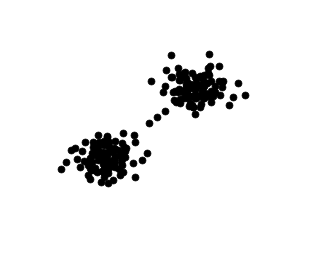
\includegraphics[width=.3\linewidth]{imagenes/c2/TwoBasicsClusters}}
	{
\includegraphics[width=.3\linewidth]{imagenes/c2/MoonsBasics}}
	{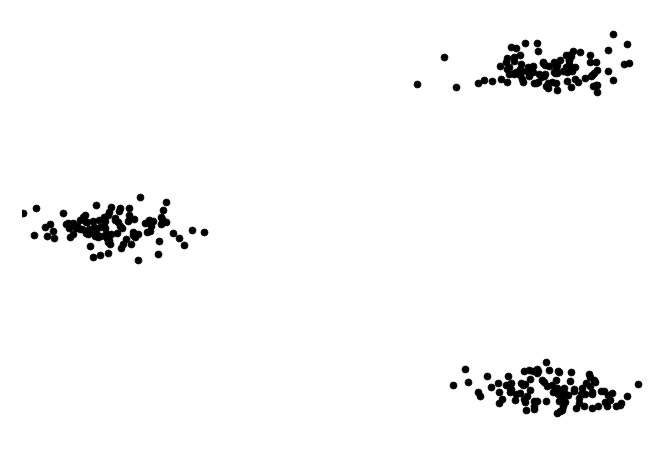
\includegraphics[width=.3\linewidth]{imagenes/c2/ThreeBasicClusters}}
	\caption[Clusters con cohesión interna y/o aislamiento externo]{Clusters con cohesión interna y/o aislamiento externo}\label{fig:figure1}
\end{figure}

Por otra parte, como ya mencionamos anteriormente en esta sección, puede darse el caso de que en un conjunto de datos no exista una partición justificada. En la Figura \ref{fig:figure2} se muestra un conjunto de datos para el que la mayoría de observadores llegaría a la conclusión de que no existen grupos diferenciados, simplemente una nube de puntos uniformemente distribuidos. Idealmente, es de esperar que un método de clustering aplicado a este mismo conjunto de datos llegue a la misma conclusión.

\begin{figure}[!h]
	\centering
	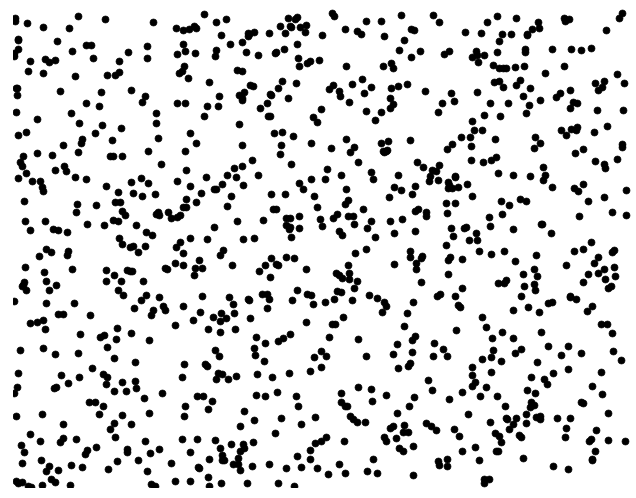
\includegraphics[scale=0.2]{imagenes/c2/rand.png} 
	\caption{Distribución uniforme de puntos}\label{fig:figure2}
\end{figure}

Sin embargo, la mayoría de métodos de aprendizaje no supervisado darán como resultado un particionamiento uniforme como el que se muestra en la Figura \ref{fig:figure3}. El número de particiones encontradas dependerá del método aplicado, si bien en cualquier caso obtendremos un particionamiento uniforme.

\begin{figure}[!h]
	\centering
	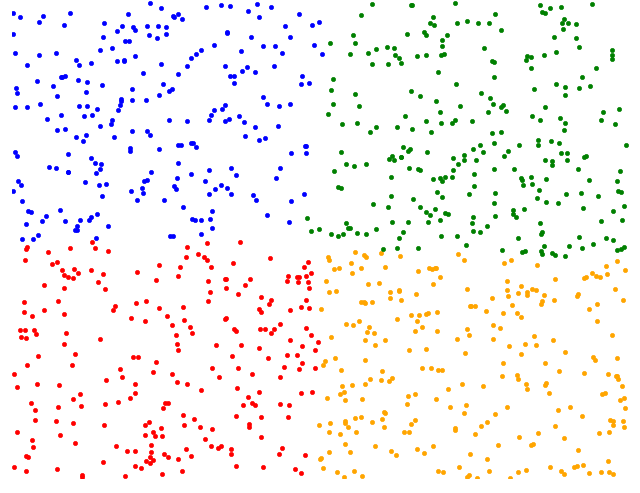
\includegraphics[scale=0.2]{imagenes/c2/randClasif.png} 
	\caption{Distribución uniforme de puntos clasificados}\label{fig:figure3}
\end{figure}

El proceso de dividir una distribución homogénea de datos en diferentes grupos se conoce como disección, y tal proceso puede ser útil en ciertas circunstancias. Sin embargo, dado que en la mayoría de las ocasiones de aplicación real de métodos de clusters, no se conoce a priori la estructura de los datos, existe el riesgo de interpretar todas las soluciones en términos de existencia de subgrupos, lo que conllevaría la imposición de una estructura ficticia en datos en los que no hay estructura presente.

\section{Aplicaciones del clustering}

Como ya se ha indicado, el problema general al que intenta dar solución el clustering está presente en muchas disciplinas: biología, botánica, medicina, psicología, geografía, marketing, procesamiento de imágenes, psiquiatría, arqueología, etc. En esta sección se presentan algunas de las aplicaciones del clustering relacionadas con los citados campos.

\subsection{Aplicaciones en marketing}

Dividir los clientes en grupos homogéneos es una de las tareas más frecuentes en marketing. Un director de marketing podría preguntarse cómo agrupar los posibles clientes según los beneficios potenciales del producto que intenta introducir en el mercado. Por otra parte, un analista de marketing podría estar interesado en agrupar las empresas según sus características financieras, para poder analizarlas y predecir sus estrategias de mercado.

Un ejemplo de aplicación del clustering en este ámbito fue publicado por Green et al. (1967). Así, con un gran número de ciudades disponibles para el análisis, debieron restringir los lugares en los que llevar a cabo sus estudios debido a motivos económicos. Para ello hicieron uso del análisis de clusters, clasificando las ciudades en pequeños grupos basándose en 14 características de las mismas, entre ellas el tamaño e ingresos medios \textit{per capita}. Dado que se esperaba que las ciudades incluidas en un mismo grupo fueran muy similares, escogieron una ciudad de cada uno de ellos para realizar sus estudios.

Otra aplicación del análisis de clusters en el marketing fue descrita por Chakrapani (2004). En este caso, un fabricante de coches cree que comprar un coche deportivo no es una decisión basada sólo en capacidades económicas o edad, sino que es una decisión relacionada con el estilo de vida que llevan aquellos que deciden comprar un coche de estas características, frente a aquellos que no lo hacen. En consecuencia, el fabricante decide realizar un estudio, empleando análisis de clusters, que le permita identificar todas las características relacionadas con las personas que comprarían un coche deportivo, para así enfocar sus campañas de marketing a este sector específicamente.

\subsection{Aplicaciones en astronomía}

Dado un conjunto de datos astronómicos, los investigadores quieren saber, por ejemplo, cuantas clases de estrellas hay presentes en ellos, basándose en algun criterio estadístico. Las preguntas más frecuentes dentro de este ámbito son: ¿Cuantos objetos estadísticamente diferentes están presentes en los datos y a qué clase debe ser asignado cada objeto? ¿Aparecen clases de objetos previamente desconocidas?. El análisis de clusters puede ser aplicado para dar respuesta a estas cuestiones, ayudando a detectar objetos estadísticamente anómalos, así como a guiar el proceso de clasificación de los mismos. Algunos ejemplos incluyen el descubrimiento de quasars con alto corrimiento al rojo, quasars de tipo 2 (altamente luminosos, núcleos galácticos activos a menudo oscurecidos por polvo y gas), y enanas marrones.

Un ejemplo específico viene dado por el estudio de Faúndez-Abans et al. (1996), quienes aplicaron técnicas de clustering a datos sobre la composición química de 192 nebulosas planetarias. Se identificaron 6 grupos diferentes que eran similares en muchos aspectos a una clasificación previa de dichos objetos, pero que también mostraban diferencias interesantes que hasta ese momento los investigadores habían pasado por alto.

Un segundo ejemplo lo encontramos en el estudio de Celeux y Govaert (1992), quienes aplicaron clustering basado en distribuciones normales a un conjunto de 2370 estrellas, descritas por su velocidad relativa al núcleo galáctico y a la rotación galáctica. Usando un modelo de tres clusters, encontraron un cluster de gran tamaño y pequeño volumen, y dos de pequeño tamaño y gran volumen.

\subsection{Aplicaciones en psiquiatría}

Las enfermedades de la mente son a menudo más difíciles de diagnosticar que las enfermedades del cuerpo; es por ello que en el campo de la psiquiatría ha crecido el interés por las técnicas de análisis de clusters que permitan refinar, o incluso redefinir, las técnicas de diagnosis para este tipo de enfermedades. Gran parte de este trabajo involucra pacientes deprimidos, casos en los que el interés reside en distinguir entre dos tipos de depresión, la endógena (congénita), y la neurótica.

Pilowsky et al. (1968), por ejemplo, usando métodos desarrollados por otros autores, aplicaron técnicas de clustering a 200 pacientes en base a sus respuestas a un cuestionario sobre la depresión, junto a información sobre su sexo, edad, estado mental y enfermedad padecida. Éste es un claro ejemplo de variables de diferentes tipos incluidas en el mismo conjunto de datos. Uno de los grupos obtenidos como resultado de este estudio fue identificado como marcador de la depresión endógena.

El análisis de clusters también ha sido empleado para encontrar una clasificación de individuos que intentaron cometer suicidio, que podría sentar las bases para estudios posteriores sobre las causas y tratamientos del problema. Paykey y Rassaby (1978), por ejemplo, estudiaron 236 casos de suicidas fallidos registrados por el servicio de emergencias de una ciudad de los Estados Unidos de América. Del conjunto de posibles variables, 14 fueron seleccionadas como particularmente relevantes para la clasificación y, por tanto, fueron usadas en el análisis. Entre ellas se encontraban: edad, número de intentos de suicidio, gravedad de la depresión y grado de hostilidad, además de una serie de características demográficas. Al conjunto de datos resultante se le aplicó métodos de clustering; el resultado más significativo obtenido corresponde a una división en tres clusters bien definidos.

\subsection{Aplicaciones en meteorología y climatología}

Diariamente se recogen enormes cantidades de datos sobre la meteorología mundial. Explorar estos datos mediante técnicas de clustering puede aportar nuevos enfoques para la climatología y el medio ambiente.

Littmann (2000), por ejemplo, aplicó clustering a los datos recogidos sobre los cambios diarios en la presión superficial en la cuenca Mediterránea, y encontró 20 grupos que explicaban la varianza de las lluvias en las regiones centrales del Mediterráneo. Otro ejemplo viene de la mano de Liu y George (2005), quienes usaron el algoritmo K-medias difuso (\textit{Fuzzy K-means}, \acs{FKM}) con datos espaciotemporales de la climatología de las regiones del sur central de EEUU. 

\subsection{Aplicaciones en arqueología}

La arqueología es otra de las disciplinas en la que resulta útil la aplicación del clustering. La clasificación de los diferentes objetos encontrados en los yacimientos puede ayudar a descubrir su uso, los periodos a los que pertenecen, así como la población que los utilizó. De forma similar, el estudio de materiales fosilizados puede ayudar a revelar como vivieron las sociedades prehistóricas. 

Un ejemplo temprano de la aplicación de clustering a objetos arqueológicos viene dado por Hodson et al. (1966), quienes aplicaron técnicas de clustering a un grupo de broches que datan de la Edad de Hierro, encontrando una clasificación para los mismos de demostrada relevancia arqueológica. Otro ejemplo de la mano de Hodson (1971) es la aplicación del algoritmo K-medias (\acs{KM}, Apéndice \ref{ap:kmeans}) para construir una taxonomía de hachas de mano encontradas en las Islas Británicas. Las variables tenidas en cuenta para describir cada hacha incluyen longitud, anchura y valores en una escala que describen cómo de puntiaguda era la herramienta. El clustering dio como resultado dos grupos de hachas, uno formado por las pequeñas y delgadas, y otro formado por las grandes y gruesas.

Respecto a materiales fosilizados, Sutton y Reinhard (1995) realizaron un estudio sobre 155 coprolitos encontrados en \textit{Antelope House}, un yacimiento prehistórico en el Cañón de Chelly en Arizona. El estudio arrojó como resultado una interpretación de las diferencias entre coprolitos basada en la alimentación.

\subsection{Aplicaciones en bioinformática y genética}

Tiempos recientes están siendo testigo de un tremendo auge en el interés por la Bioinformática, acompañada por la biología molecular, ciencias de la computación, matemáticas y estadística. Tal aumento ha sido acelerado por la siempre creciente base de datos genómica y proteica, que son por sí mismas resultado de un grandísimo avance en las técnicas de secuenciación del ADN, medidas de expresión de los genes y compresión de las estructuras macromoleculares. La estadística ha resultado relevante en el estudio de la expresión de los genes. Los genes contenidos en el ADN de cada célula proporcionan las plantillas necesarias para la generación de las proteínas implicadas en la mayoría de los procesos estructurales y biomecánicos que tienen lugar en cada uno de nosotros. Sin embargo, aunque la mayoría de las células en los seres humanos contienen todos los complementos genéticos que componen el genoma humano, los genes se expresan de manera selectiva en cada célula dependiendo del tipo de la misma, del tejido y de las condiciones generales tanto dentro como fuera de la célula. La biología molecular ha puesto de manifiesto que la mayoría de los procesos en la vida de una célula están regulados por factores que afectan a la expresión de sus genes.

Como hemos visto, uno de los campos de investigación más activos hoy en día es el que estudia los procesos que regulan la expresión de los genes. Con el fin de almacenar la información relativa a esta área de estudio surgen los microarrays, (Cortesse, 2000). Desde el punto de vista del análisis de datos, una de las características relevantes en este tipo de información es que el número de atributos de cada instancia ($p$), supera con creces al número de instancias disponibles ($n$); conjuntos de datos como este son calificados como \textit{datos de alta dimensionalidad}.

La mayoría de métodos estadísticos clásicos no pueden ser aplicados a este tipo de conjuntos de datos sin ser modificados de forma sustancial. Sin embargo, el análisis de clusters acepta bien tales conjuntos de datos y puede ser empleado para identificar grupos de genes con patrones de expresión similares, y dar respuesta a preguntas como por qué un gen se ve afectado por cierta enfermedad, o qué genes son responsables de enfermedades genéticas hereditarias.

Un ejemplo de aplicación lo encontramos en el trabajo de Selinski e Ickstadt (2008), quienes usaron clustering sobre polimorfismos de nucleótidos simples para detectar diferencias entre enfermedades a nivel genético.

\section{Resumen}

El clustering consiste en la exploración de conjuntos de datos. Su objetivo es discernir si pueden o no ser resumidos de manera significativa, en términos de un número relativamente pequeño de grupos o clusters de objetos o individuos, que se parecen unos a otros y que se diferencian de los que se encuentran en otros clusters.

Muchas ramas de la ciencia han hecho uso de las técnicas de clustering de manera exitosa, para avanzar en sus respectivos campos, y procesar grandes cantidades de datos, cuyo análisis sería impensable afrontar con técnicas tradicionales.

%Para referir un acronimo completo \acf
%Para referir un acronimo solo con las siglas \acs





















\chapter{Clustering con restricciones}\label{ch:Clustering con restricciones}

Realizada la introducción sobre los conceptos básicos del clustering, el objetivo de este capítulo es definir los conceptos relacionados con el clustering con restricciones, así como dar ejemplos de su aplicación y destacar los beneficios y problemas que presenta su uso. A tal fin tomamos como referencia principal el trabajo de Ian Davidson y Sugato Basu (2007) \cite{Survey:2007} entre otros.

\section{Motivación para el clustering con restricciones}

Tal y como hemos estudiado en el Capítulo \ref{ch:Breve introducción al Clustering}, los métodos de clustering no supervisado son útiles para dotar de estructura a datos referentes a un área concreta. Un ejemplo de ello lo encontramos en la clasificación de textos; Cohn et al. (2003) \cite{Cohn:2003} afrontan un problema propuesto por Yahoo!, que consiste en, dada una gran cantidad de documentos de texto, agruparlos según una taxonomía en la que los documentos con temáticas similares se encuentren cercanos. Para ello, los métodos de clustering no supervisado resultan de utilidad, ya que la información sobre el problema de la que se dispone inicialmente es limitada. Sin embargo, Wagstaff et al. (2001) mostraron que aplicando clustering no supervisado a ciertos problemas, como el de agrupar datos de GPS de forma que los clusters definan los carriles de una vía, no se obtienen resultados significativos, pues los clusters obtenidos distan mucho de la forma alargada que se esperaría como resultado. Para atajar el problema, introdujeron en el clustering un nuevo elemento, las restricciones a nivel de instancia, que permitían incluir conocimiento sobre los clusters que guiarían los métodos de clustering para obtener los resultados esperados. Bastaba con indicar que los carriles de la vía por la que circulan los vehículos miden cuatro metros de ancho, y por tanto cualquier vehículo que se encuentre a una distancia mayor de 4 metros de otro, en dirección perpendicular a la del desplazamiento, debe ser ubicado en un cluster diferente.

Nos situamos entonces en un nuevo escenario: es posible incorporar información adicional al proceso de clustering, además de la contenida en el propio conjunto de datos, para guiarlo en la formación de la partición y obtener resultados más precisos. Esto sitúa al clustering con restricciones en el marco del aprendizaje semisupervisado, a diferencia de los métodos de clustering tradicionales que se enmarcan en el área del clustering no supervisado. 

\section{Definición de las restricciones}

El nuevo tipo de  información que incorporamos al clustering viene dado en forma de restricciones a nivel de instancia, esto es, especificar si dos instancias del conjunto de datos deben estar en el mismo cluster o, por el contrario, deben estar en clusters separados.

A las restricciones que indican que dos puntos deben ser situados en el mismo cluster se las denomina \textit{Must-link}, y se notan con $ML(x,y)$, donde $x$ e $y$ son dos instancias del conjunto de datos. De manera similar, a las restricciones que especifican lo contrario se las denomina \textit{Cannot-link}, y se notan con $CL(x,y)$. \cite{WagstaffCardie:2000}

Aunque pueden parecer simples, las restricciones definidas de la anterior forma poseen propiedades interesantes. Las Restricciones de tipo Must-link son un ejemplo de relación de equivalencia, y por tanto son simétricas, reflexivas y transitivas, formalizando:

\begin{observacion}
	\textbf{Las restricciones de tipo ML son transitivas.} Sean $CC_i$ y $CC_j$ componentes conexas, conectadas mediante restricciones $ML$, y sean $x$ e $y$ dos instancias en $CC_i$ y $CC_j$ respectivamente. Entonces $ML(x,y): x \in CC_i, y \in CC_j \rightarrow ML(a,b) \forall a,b: a\in CC_i, b \in CC_j$. \cite{Survey:2007}
\end{observacion}

\begin{observacion}
	\textbf{Las restricciones de tipo CL pueden ser deducidas.} Sean $CC_i$ y $CC_j$ componentes conexas, conectadas mediante restricciones $ML$, y sean $x$ e $y$ dos instancias en $CC_i$ y $CC_j$ respectivamente. Entonces $CL(x,y): x \in CC_i, y \in CC_j \rightarrow CL(a,b) \forall a,b: a\in CC_i, b \in CC_j$. \cite{Survey:2007}
\end{observacion}

Un claro ejemplo de uso de las restricciones lo encontramos en casos de aplicación de clustering en los que existen limitaciones en cuanto a las medidas de distancia, como sucedía en el supuesto de los datos GPS. Así, si queremos que las instancias que forman dos clusters estén separadas por una distancia mayor o igual a $\delta$, basta con establecer restricciones de tipo ML entre todas aquellas instancias cuya distancia sea menor que $\delta$. 
De manera similar, si queremos que el diámetro de los clusters sea como mucho $\epsilon$, debemos establecer un conjunto de restricciones de tipo CL entre todas aquellas instancias que se encuentren a una distancia mayor que $\epsilon$. La Figura \ref{fig:figure4} muestra una representación gráfica de estos dos tipos de restricciones.

\begin{figure}[!h]
	\centering
	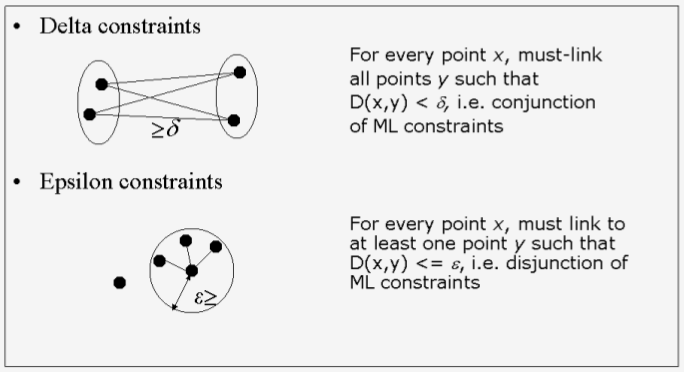
\includegraphics[scale=0.45]{imagenes/c3/RestriccionesDeltaEpsilo.png} 
	\caption[Restricciones de tipo \textit{delta} y \textit{épsilon}.]{Restricciones de tipo \textit{delta} y \textit{épsilon}. \cite{Survey:2007}}\label{fig:figure4}
\end{figure}


\section{Uso de las restricciones}

Mientras que el aprendizaje completamente supervisado implica conocer la etiqueta asociada a cada instancia, en el aprendizaje semisupervisado sólo se dispone de un subconjunto de instancias etiquetadas. Por otra parte, en gran cantidad de dominios la información disponible se refiere a relaciones entre instancias, y no a la clase concreta a la que pertenecen las mismas. Es más, en sistemas de clustering interactivo, un usuario no experto en el dominio del problema podrá, probablemente, aportar información en forma de restricciones de tipo \acf{ML} y \acf{CL} \cite{Cohn:2003}\cite{DavidsonRavi:2007}, antes que aportar información sobre a qué clase concreta pertenecen ciertas instancias.

Habitualmente, las restricciones se incluyen en los problemas de clustering de dos maneras. Pueden ser empleadas para modificar la regla de asignación de instancias a clusters del método en cuestión, de forma que la solución satisfaga el máximo número de restricciones posible. Alternativamente, cabe la posibilidad de entrenar la función de distancia empleada por el método en base a las restricciones, ya sea antes o durante la aplicación del mismo. En cualquier caso, la fase de inicialización puede tomar en consideración las restricciones, de forma que las instancias asociadas con restricciones \acf{ML} serán situadas en el mismo cluster, y aquellas entre las que exista una restricción \acf{CL}, quedarán en clusters diferentes. Basándonos en esta distinción, identificamos dos maneras de aproximar el problema, las basadas en restricciones (\textit{constraint-based}), y las basadas en distancias (\textit{distance-based}).

\subsection{Métodos basados en restricciones}

En los métodos basados en restricciones, el propio método de clustering es modificado de manera que la información disponible se emplea para sesgar la búsqueda y obtener una partición de los datos apropiada.

Existen dos modelos de métodos basados en restricciones: (1) aquellos que fuerzan el cumplimiento de las restricciones, e intentan encontrar la mejor asignación posible que no infrinja ninguna de ellas \cite{Wagstaff:2001b}\cite{DavidsonRavi:2005b}, y (2) los que hacen una interpretación relajada de las restricciones \cite{Basu:2004}\cite{Seagal:2003}\cite{DavidsonRavi:2005a}\cite{Law:2005}, permitiéndose incumplir un número mínimo de ellas para optimizar la función objetivo; de esta manera surge un compromiso entre el número de restricciones incumplidas y el valor de la función objetivo. Existen diversas técnicas para obtener una partición atendiendo a las restricciones:

\begin{itemize}
	
	\item Modificar la función objetivo de manera que incluya una penalización por incumplir restricciones. \cite{Demiriz:1999} \cite{DavidsonRavi:2005a}
	
	\item Agrupar instancias con información adicional obtenida de una distribución condicional en un espacio auxiliar. \cite{SinkkonenKaski:2000}
	
	\item Forzar el cumplimiento de todas las restricciones modificando la regla de asignación del método. \cite{Wagstaff:2001b}
	
	\item Inicializar los clusters en base a restricciones inferidas del conjunto de instancias etiquetadas.\cite{Basu:2002}
	
\end{itemize}

La Figura \ref{fig:figure5} muestra un conjunto de datos junto a sus restricciones asociadas. La Figura \ref{fig:figure6} propone un posible agrupamiento que satisface todas las restricciones.

\begin{figure}[bth]
	\myfloatalign
	{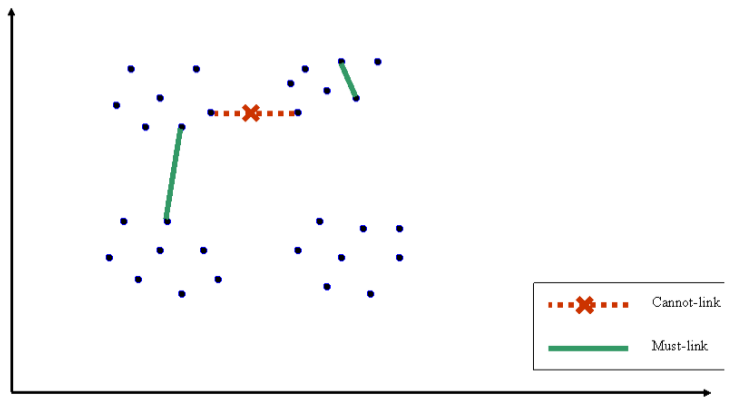
\includegraphics[width=.6\linewidth]{imagenes/c3/InputInstancesAndConst1}
	\caption[Restricciones sobre un conjunto de datos.]{Restricciones sobre un conjunto de datos. \cite{Survey:2007}} \label{fig:figure5}
	}
	{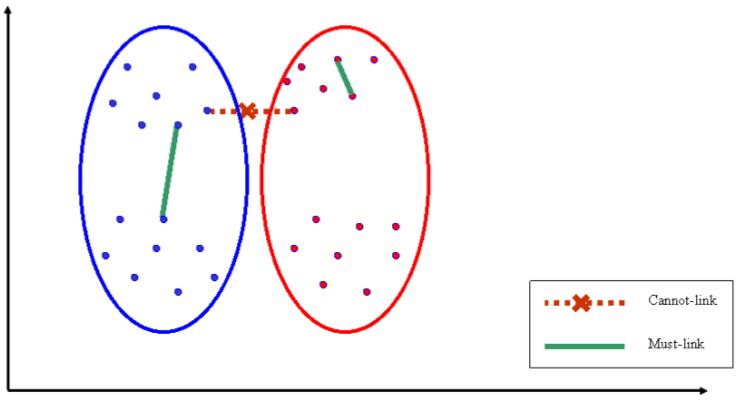
\includegraphics[width=.6\linewidth]{imagenes/c3/ClusteringSatAll}
	\caption[Clustering que satisface todas las restricciones.]{Clustering que satisface todas las restricciones. \cite{Survey:2007}} \label{fig:figure6}
	}
\end{figure}

\subsection{Métodos basados en distancia}

En las aproximaciones basadas en distancias se emplean métodos de clustering clásicos que hacen uso de una medida de distancia, de forma que dicha medida se modifica para que tenga en consideración las restricciones. En este contexto, satisfacer las restricciones significa que las instancias relacionadas con restricciones \acf{ML} se sitúan juntas en el espacio, y las relacionadas mediante \acf{CL} se encuentran separadas.

La Figura \ref{fig:figure8} muestra un posible agrupamiento basado en una métrica aprendida a partir de las restricciones especificadas en la Figura \ref{fig:figure7}. Cabe destacar que en la Figura \ref{fig:figure8} el espacio en el que se encuentran los datos ha sido comprimido en el eje vertical y ensanchado en el eje horizontal para ajustarlo a la métrica de distancia aprendida.

\begin{figure}[bth]
	\myfloatalign
	{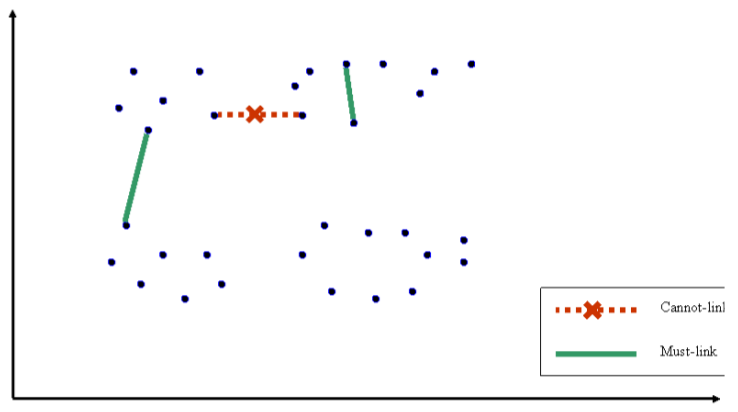
\includegraphics[width=.6\linewidth]{imagenes/c3/InputInstancesAndConst2}
	\caption[Restricciones sobre un conjunto de datos.]{Restricciones sobre un conjunto de datos. \cite{Survey:2007}} \label{fig:figure7}
	}
	{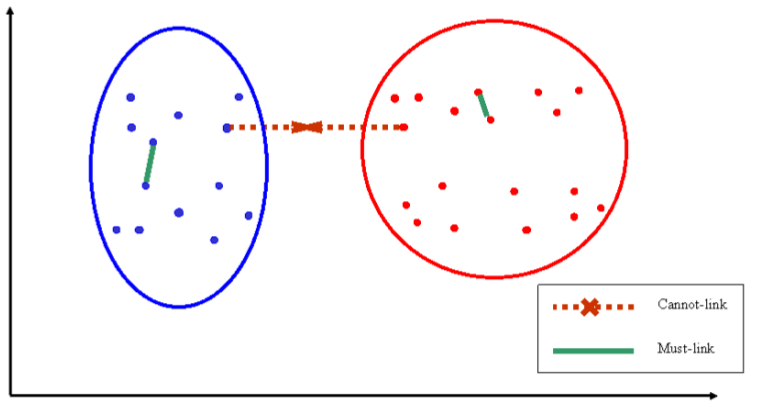
\includegraphics[width=.6\linewidth]{imagenes/c3/MetricaAprendida}
	\caption[Clustering basado en métrica aprendida en base a las restricciones.]{Clustering basado en métrica aprendida en base a las restricciones. \cite{Survey:2007}} \label{fig:figure8}
	}
\end{figure}

\section{Aplicaciones del clustering con restricciones} \label{aplicacion}

Esta sección muestra algunos casos de aplicación en los que el clustering con restricciones ha resultado ser una herramienta más útil que el clustering no supervisado. Para cada caso analizaremos cómo se obtuvieron las restricciones y cómo éstas mejoran los resultados en el clustering resultante. 

\subsection{Aplicaciones en análisis de imágenes}

La Figura \ref{fig:figure9} muestra un extracto del conjunto de datos de caras de  CMU (Carnegie Mellon University), en el que la tarea es agrupar caras en base a diferentes criterios. En este caso, el objetivo es agrupar las caras según su orientación.

\clearpage

\begin{figure}[bth]
	\myfloatalign
	\subfloat[Caras de perfil]
	{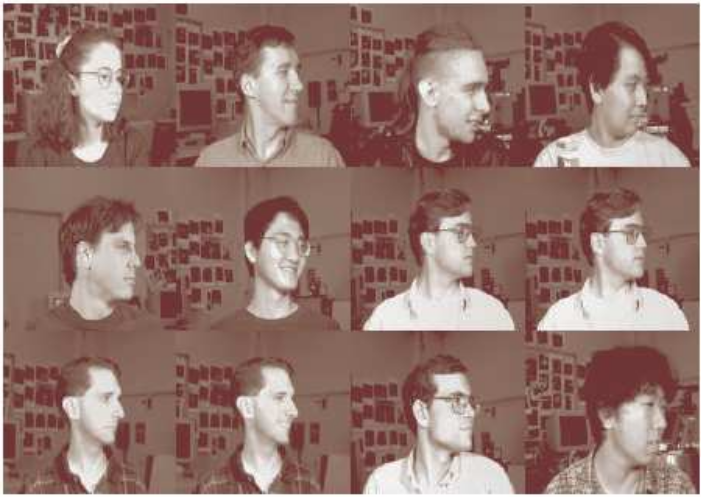
\includegraphics[width=.3\linewidth]{imagenes/c3/AnalisisImagenes/Caras1}} \quad
	\subfloat[Caras de frente.]
	{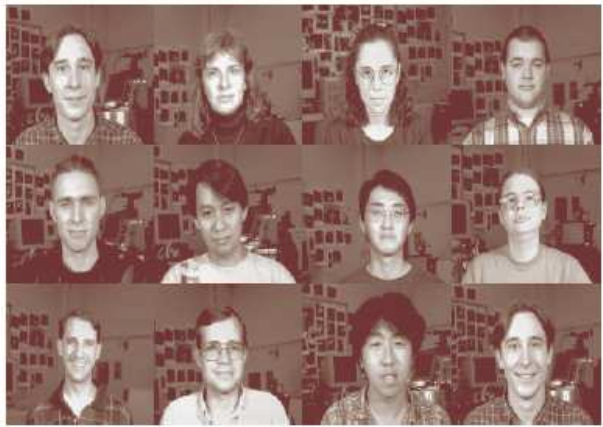
\includegraphics[width=.3\linewidth]{imagenes/c3/AnalisisImagenes/Caras3}} \quad
	\subfloat[Caras hacia arriba.]
	{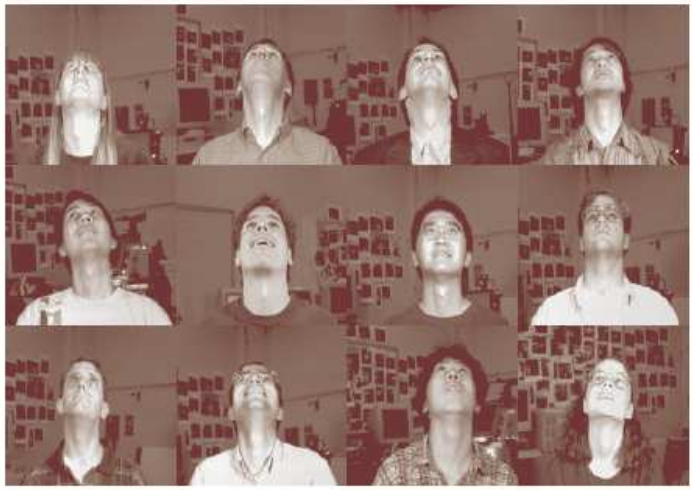
\includegraphics[width=.3\linewidth]{imagenes/c3/AnalisisImagenes/Caras2}} \quad
	\caption[Caras de la base de datos de  CMU.]{Caras de la base de datos de  CMU. \cite{Survey:2007}}\label{fig:figure9}
\end{figure}

El método empleado para extraer las restricciones es uno de los más populares en la literatura: establecer el número de clusters de la partición resultado igual al número de clases en la base de datos, y generar las restricciones a partir de un subconjunto de instancias etiquetadas; esto es, si dos instancias tiene diferentes etiquetas, establecer una restricción \acf{CL} entre ellas, en caso contrario una de tipo \acf{ML}. De esta forma, entre las imágenes mostradas en la Figura \ref{fig:figure10} se establecen restricciones \acf{CL}, ya que, aunque pertenecen a la misma persona, no presentan la misma orientación.

\begin{figure}[bth]
	\myfloatalign
	{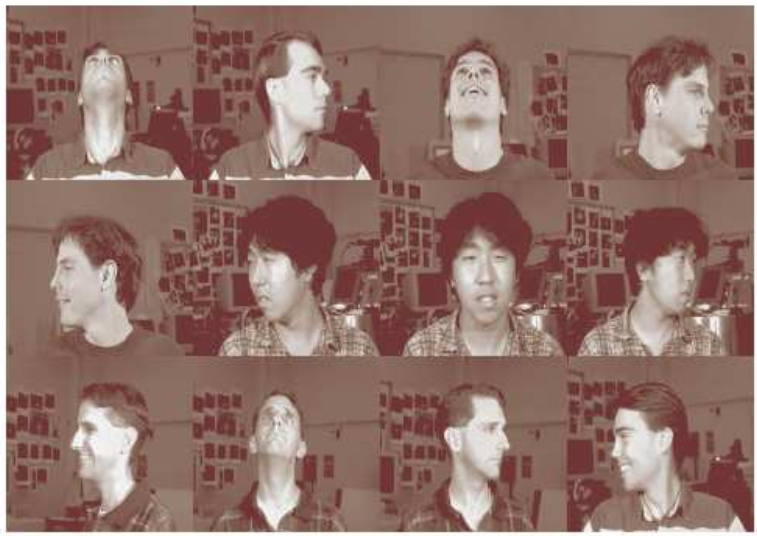
\includegraphics[width=.35\linewidth]{imagenes/c3/AnalisisImagenes/CarasDifOr1}} \quad
	{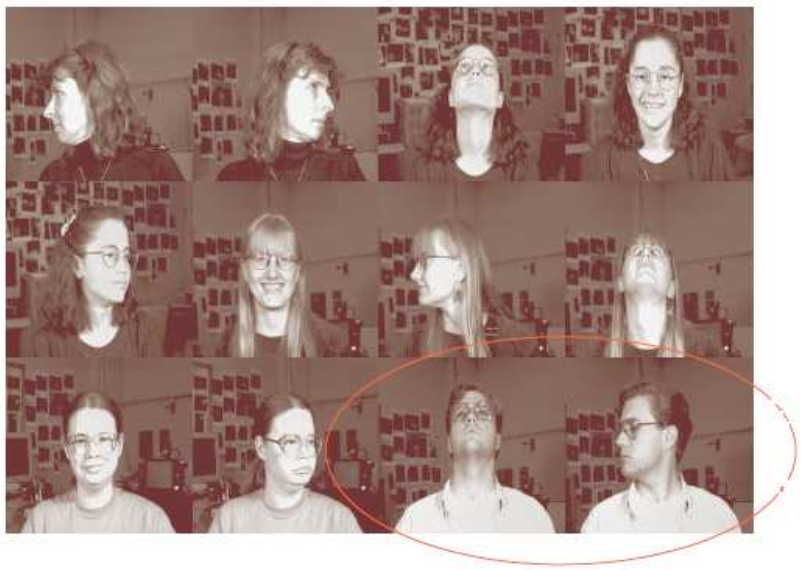
\includegraphics[width=.35\linewidth]{imagenes/c3/AnalisisImagenes/CarasDifOr2}}
	\caption[Restricciones de tipo \ac{CL} entre caras de la misma persona.]{Restricciones de tipo \ac{CL} entre caras de la misma persona.  \cite{Survey:2007}}\label{fig:figure10}
\end{figure}

En la Figura \ref{fig:figure11} se muestra otro conjunto de datos de imágenes sobre el que se aplican técnicas de clustering con restricciones. En este caso, la tarea es realizar reconocimiento de objetos para incorporar el método al sistema de navegación del robot Aibo \cite{DavidsonRavi:2005a}. Para ello se emplean restricciones de distancia de tipo $\delta$ y $\epsilon$ como las descritas en la Figura \ref{fig:figure4}. De esta manera se consiguen clusters bien diferenciados y por tanto útiles para las tareas de búsqueda de caminos que el robot realiza durante la navegación.

\begin{figure}[bth]
	\myfloatalign
	\subfloat[Imagen original]
	{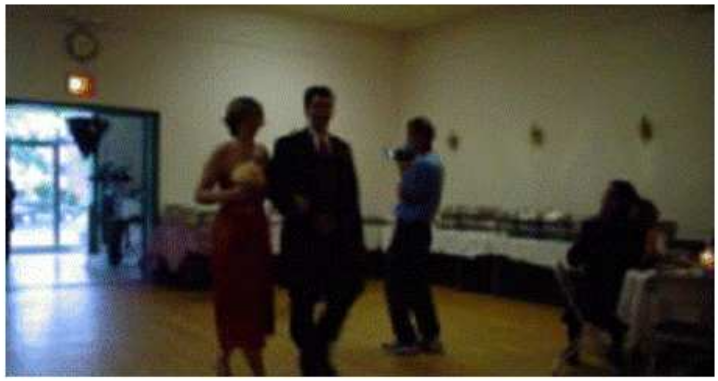
\includegraphics[width=.3\linewidth]{imagenes/c3/AnalisisImagenes/Aibo1}} \quad
	\subfloat[Clustering sin restricciones]
	{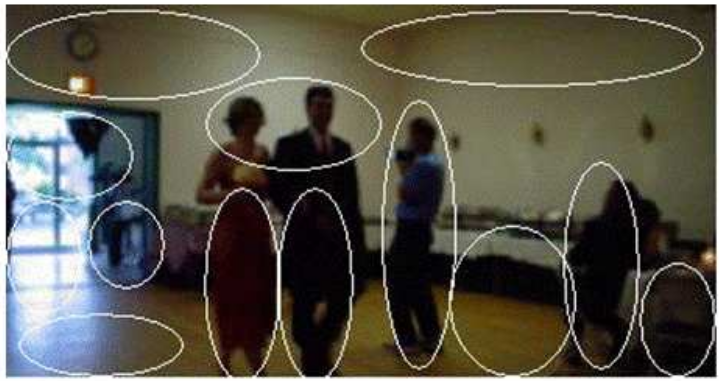
\includegraphics[width=.3\linewidth]{imagenes/c3/AnalisisImagenes/Aibo2}} \quad
	\subfloat[Clustering con restricciones]
	{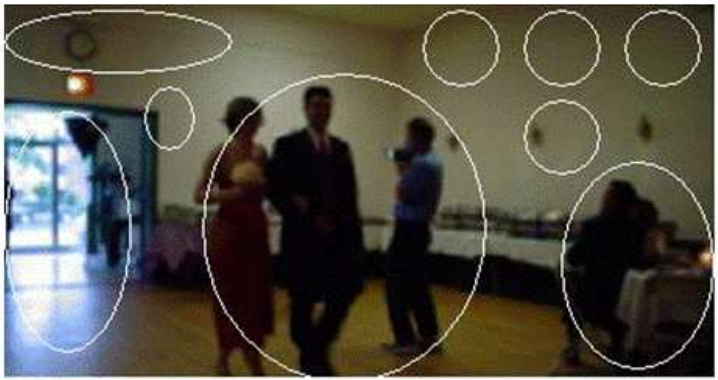
\includegraphics[width=.3\linewidth]{imagenes/c3/AnalisisImagenes/Aibo3}} \quad
	\caption[Método de clustering empleado en el sistema de navegación del robot Aibo.]{Método de clustering empleado en el sistema de navegación del robot Aibo. \cite{Survey:2007}\cite{DavidsonRavi:2005a}}\label{fig:figure11}
\end{figure}

\subsection{Aplicaciones en análisis de vídeos}

Las bases de datos de vídeo son uno de los ejemplos en los que las restricciones pueden ser generadas directamente desde el dominio de datos, especialmente disponiendo de datos espacio-temporales sobre el vídeo \cite{Yan:2006}. En datos temporalmente sucesivos es posible establecer restricciones de tipo \acf{ML} entre grupos de píxeles de fotogramas (\textit{frames}) cercanos en el tiempo. Esto es especialmente útil cuando la tarea es implementar reconocimiento de objetos basado en clustering y segmentación. También es posible añadir restricciones \acf{CL} a clusters localizados en el mismo fotograma, ya que existe una baja probabilidad de que estén asociados al mismo objeto. De hecho, en el dominio asociado a problemas de análisis de vídeo existen gran variedad de métodos de extracción de restricciones \cite{Yan:2006}, la Figura \ref{fig:figure12} muestra algunos ejemplos.  

\begin{figure}[bth]
	\myfloatalign
	\subfloat[]
	{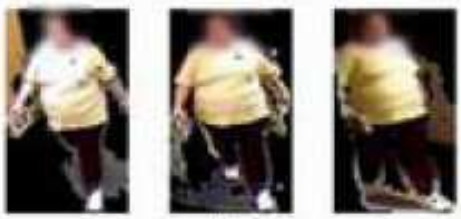
\includegraphics[width=.4\linewidth]{imagenes/c3/Videos/VideoA}}
	\quad
	\subfloat[]
	{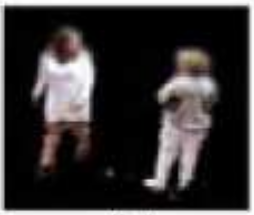
\includegraphics[width=.225\linewidth]{imagenes/c3/Videos/VideoB}} \quad
	\subfloat[]
	{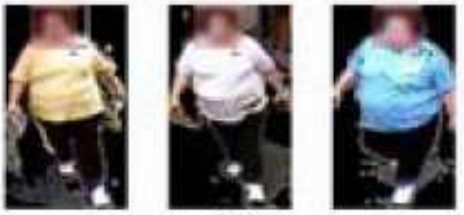
\includegraphics[width=.4\linewidth]{imagenes/c3/Videos/VideoC}}
	\quad
	\subfloat[]
	{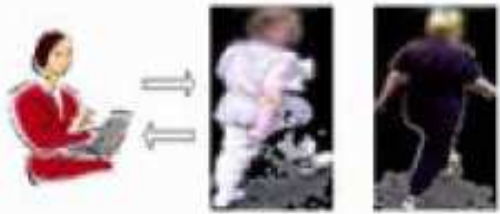
\includegraphics[width=.4\linewidth]{imagenes/c3/Videos/VideoD}}
	\caption[Diferentes tipos de restricciones en datos de video.]{Diferentes tipos de restricciones en datos de video. \cite{Yan:2006} \cite{Survey:2007}}\label{fig:figure12}
\end{figure}

En la Figura \ref{fig:figure12}, la imagen (a) corresponde a restricciones extraídas del seguimiento de una persona durante un periodo de tiempo, la (b) corresponde a restricciones espaciales que asocian dos objetos localizados en el mismo fotograma, la imagen (c) corresponde a restricciones obtenidas mediante reconocimiento facial y la (d) a las proporcionadas por el usuario.

Disponiendo de tantos métodos para extraer restricciones, cabe plantearse: ¿qué sucede si se establecen demasiadas restricciones? ¿Hace esto que el problema esté sobrerestringido? En la Sección \ref{Problemas} abordaremos estas cuestiones.

\subsection{Aplicaciones en genética}

En clustering de genes basado en microarrays, los genes vienen representados por su perfil de expresión en diferentes experimentos y agrupados empleando diferentes métodos, en este caso métodos de clustering con restricciones. La  Figura \ref{fig:figure13} muestra un ejemplo: se trata de restricciones de tipo \acf{ML} que se establecen entre genes en base a los datos de co-ocurrencia almacenados en la base de datos de interacciones de proteínas, que contiene información sobre qué genes (y sus proteínas asociadas) están presentes en los mismos procesos celulares \cite{Xenarios:2001}. Esta información puede ser empleada para mejorar los resultados que proporcionan los métodos de clustering. \cite{Seagal:2003}

\begin{figure}[!h]
	\centering
	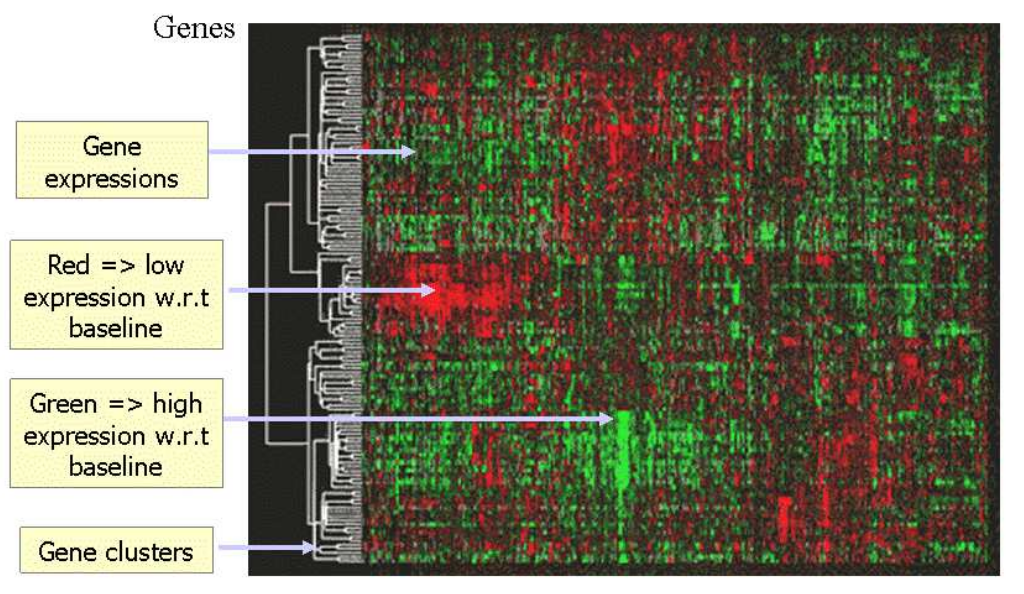
\includegraphics[scale=0.3]{imagenes/c3/Genetica/Genes} 
	\caption[Clustering de genes basado en microarrays.]{Clustering de genes basado en microarrays. \cite{Survey:2007}}\label{fig:figure13}
\end{figure}

\subsection{Aplicaciones en análisis de textos}

En tareas de clasificación de contenido, el objetivo es dividir de manera automática grandes cantidades de documentos en grupos o clusters. En este caso es posible extraer las restricciones de múltiples recursos auxiliares. Por ejemplo, si dos documentos se encuentran en el mismo directorio se podría inferir una restricción de tipo \acf{ML} entre ellos. De esta manera es posible modificar el clustering resultante para que se adapte a un criterio concreto, como por ejemplo crear una jerarquía de documentos semejante a la forma en la que se encuentran organizados en la estructura de directorios de entrada.

\subsection{Aplicaciones en datos web} 

El clustering con restricciones resulta de gran utilidad en el procesamiento de datos de búsqueda en páginas web. Aquí, el objetivo es agrupar, de manera automática, los resultados de una consulta ambigua en el motor de búsqueda en clusters de \acs{URL}s, que se refieran al concepto introducido como consulta en diferentes contextos. En este ámbito es posible extraer las restricciones a partir de búsquedas realizadas anteriormente por los usuarios, de manera que se establece una restricción de tipo \acf{ML} entre \acs{URL}s visitadas en la misma sesión de usuario. Aplicar clustering utilizando estas restricciones puede ayudar a sesgar el resultado de las búsquedas hacia las preferencias del usuario.

\subsection{Aplicaciones en datos de audio}

En ciertas tareas de análisis de audio, es posible que no se conozca el número de clases de objetos presentes en los datos, si bien las restricciones pueden extraerse directamente del dominio de datos. Esto sucede, por ejemplo, al aplicar clustering para reconocimiento de hablantes en una conversación \cite{BarHillel:2003}. En este caso el número de participantes no se conoce a priori, pero es fácil detectar si dos hablantes son diferentes o similares y establecer las restricciones en base a ello.

\subsection{Aplicaciones en datos de GPS} \label{EjemploGPS}

Tal y como se indicó en el inicio del Capítulo \ref{ch:Clustering con restricciones}, el clustering con restricciones sobre datos \acs{GPS} se utiliza para identificar el carril por el que circula cada vehículo, como se muestra en la Figura \ref{fig:figure14}. Cada instancia viene representada por la posición que ocupa en la vía en coordenadas cartesianas bidimensionales $(x,y)$, obtenidas en base a los datos \acs{GPS}. La Figura \ref{fig:figure15} muestra de manera gráfica esta representación de los datos (cabe destacar que múltiples instancias pueden referirse al mismo vehículo en distintos momentos en el tiempo).

\begin{figure}[!h]
	\centering
	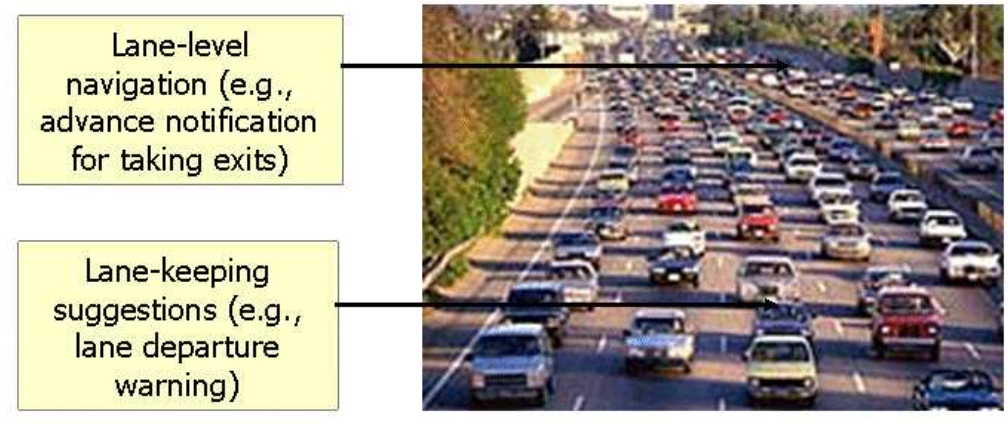
\includegraphics[scale=0.3]{imagenes/c3/GPS/Coches} 
	\caption[Uso de información GPS.]{Uso de información GPS. \cite{Survey:2007} \cite{Wagstaff:2001b}}\label{fig:figure14}
\end{figure}


En este dominio, los clusters reales tiene forma alargada en el eje horizontal y se encuentran alineados perpendicularmente a la dirección de desplazamiento. Para lograr que los clusters resultantes tengan esta forma, podemos hacer uso de las restricciones. Estableceremos una restricción de tipo \acf{CL} entre aquellas instancias separadas más de 4 metros en dirección perpendicular a la del desplazamiento (ya que los carriles tiene una anchura máxima de 4 metros), y \acf{ML} entre aquellas instancias que presenten continuidad en el eje horizontal, puesto que es probable que los vehículos que representan se encuentren en el mismo carril. Este modelo de clustering ha probado ser muy útil en navegación en tiempo real \cite{Wagstaff:2001b}, permitiendo notificar al usuario cuando debe cambiar de carril, o cuando no debe abandonarlo.

\begin{figure}[!h]
	\centering
	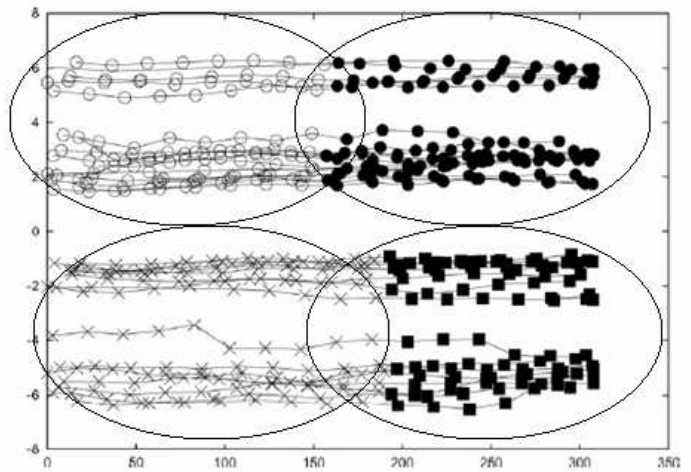
\includegraphics[scale=0.32]{imagenes/c3/GPS/Instancias} 
	\caption[Clusters encontrados en datos GPS sin uso de restricciones.]{Clusters encontrados en datos \acs{GPS} sin uso de restricciones. \cite{Survey:2007} \cite{Wagstaff:2001b}}\label{fig:figure15}
\end{figure}

\section{Beneficios del uso de restricciones}

Encontramos dos beneficios principales en el uso de restricciones: 

\begin{itemize}
	
	\item Incremento de la exactitud en las predicciones de las etiquetas al generar restricciones en base a un subconjunto de instancias etiquetadas.
	
	\item Obtención de clusters con geometría adaptable a cada problema.
	
\end{itemize}

A continuación se analizan estos dos beneficios:

Dado $X = \{x_1 \cdots x_u\}$, un gran conjunto de instancias no etiquetadas, y $L = \{(x_{u+1}, y_{u+1})\cdots (x_{u+l}, y_{u+l})\}$, un pequeño conjunto de instancias etiquetadas, es común escoger dos elementos de $L$ (con reemplazamiento) y establecer una restricción \acs{ML} entre ellos si pertenecen a la misma clase o, en caso contrario, una de tipo \acs{CL}. Un método apropiado para evaluar los resultados ofrecidos por un método de clustering es medir el nivel de exactitud de éste a la hora de predecir las etiquetas del conjunto $X$. Esto normalmente requiere que se especifique el número de clusters deseados igual al número de clases conocidas en $X$ ($K = K^*$). Para medir la exactitud se emplean métodos como \textit{Rand Index} \cite{Rand:1971}.

El trabajo de Wagstaff y Cardie \cite{WagstaffCardie:2000}, en el que generaban las restricciones de la manera descrita anteriormente, demostraba que, cuando se realiza un promedio de la exactitud de las predicciones obtenidas con algoritmos de clustering con restricciones, variando estas últimas entre experimentos, se obtienen resultados hasta un 20\% mejores que con las técnicas clásicas.

\begin{observacion}
	
	\textbf{El uso de restricciones, en promedio, incrementa la precisión.}
	El rendimiento de un método al predecir etiquetas aumenta cuando se promedia empleando numerosos conjuntos de restricciones diferentes. \cite{Survey:2007}
	\label{ob:observacion33}
	
\end{observacion}

Esta regla, sin embargo, no es cierta en todos los casos, pues en conjuntos de datos como \textit{Tic-Tac-Toe Endgame}, no se consigue ningún incremento en las predicciones sea cual sea el número de restricciones empleadas. La explicación dada por los autores citados para estas excepciones se basa en que establecer $K = K^*$ no es apropiado en este caso.

El otro beneficio que reporta el uso de restricciones es la posibilidad de obtener clusters con la geometría deseada, como el ejemplo de aplicar clustering a datos \acs{GPS}, analizado en la Sección \ref{EjemploGPS} de este trabajo.

\section{Problemas del uso de restricciones} \label{Problemas}

Aunque, tal y como hemos comprobado, la incorporación de restricciones a los métodos de clustering reporta beneficios en algunas aplicaciones, existen dos inconvenientes principales que se exponen a continuación, así como posibles soluciones a los mismos.

\subsection{El problema de la factibilidad}

La introducción de restricciones en el clustering cambia el problema al que éste da solución, que pasa a ser: \textit{Encontrar la mejor partición que satisfaga todas las restricciones}. De esta manera, si aquellas no están bien especificadas o si los métodos de extracción son inadecuados, podemos encontrar que las restricciones se contradicen, lo que deriva en que no existe una asignación de instancias a clusters que las satisfaga todas. Por ejemplo, no existe asignación que satisfaga las restricciones $ML(x_1,x_2)$ y $CL(x_1,x_2)$, independientemente del valor de $K$. Lo mismo sucede para $K = 2$, y las restricciones $CL(x_1, x_2)$, $CL(x_2, x_3)$ y $CL(x_1, x_3)$. Formalizando, el problema de la factibilidad para problemas de clustering (no jerárquico) con restricciones viene definido por:

\begin{definicion}
	
	\textbf{Problema de la factibilidad para clustering con restricciones:} Dado un conjunto de datos $X$, un conjunto de restricciones $R$, un umbral superior $K_l$ y un umbral superior $K_u$ para el número de clusters resultantes, ¿Existe una partición de $X$ en bloques tal que $K_l \le K \le K_u$ y todas las restricciones en $R$ se satisfacen? \cite{DavidsonRavi:2005a} \cite{Survey:2007}
	
\end{definicion}

La complejidad teórica del problema dependerá del tipo de restricciones que se combinen en él. La Tabla \ref{tab:tabla1} presenta, de manera resumida, la complejidad esperada en cada caso. 

\begin{table}[h]
	\centering
	\setlength{\arrayrulewidth}{1mm}
	\setlength{\tabcolsep}{10pt}
	\renewcommand{\arraystretch}{1}
	
	\rowcolors{2}{gray!25}{white}
	\begin{tabular}{ >{\centering\arraybackslash}m{4cm}  >{\centering\arraybackslash}m{4cm} }
		\hline
		\rowcolor{black}
		\multicolumn{2}{c}{\bf \color{white}{Complejidad del clustering con restricciones}}\\
		\hline
		\rowcolor{gray!50}
		\textbf{Restricciones} & \textbf{Complejidad} \\
		Restricciones $\delta$ & $\mathbf{P}$ \\
		Restricciones $\epsilon$ & $\mathbf{P}$ \\
		\acs{ML} y $\delta$ & $\mathbf{P}$ \\
		\acs{ML} y $\epsilon$ & $\mathbf{NP}$-completo \\
		$\epsilon$ y $\delta$ & $\mathbf{P}$ \\
		\acs{CL} y otra & $\mathbf{NP}$-completo \\
		\hline
		
	\end{tabular}
	\caption[Complejidad del problema del clustering en función del tipo de restricciones]{Complejidad del problema del clustering en función del tipo de restricciones. \cite{Survey:2007}}
	\label{tab:tabla1}
\end{table}

Tal y como queda reflejado en la Tabla \ref{tab:tabla1}, la utilización de restricciones \acf{CL} eleva el nivel de complejidad del clustering a $\mathbf{NP}$-completo y, por tanto, el problema del clustering con restricciones es intratable. De manera intuitiva puede entenderse fácilmente que, si encontrar una sola partición que satisfaga las restricciones es un problema complejo, más complejo es aún encontrar la mejor. 

\begin{observacion}
	
	\textbf{Saber que existe una solución factible no nos ayuda a encontrarla.} Las consecuencias de este resultado sobre la complejidad del clustering con restricciones implican que, aun en caso de que exista una partición factible, no será fácil de encontrar, hablando en términos de complejidad algorítmica. \cite{Survey:2007}
	\label{ob:observacion34}
	
\end{observacion} 

Los autores Wagstaff \cite{Wagstaff:2002} y Davidson y Ravi \cite{DavidsonRavi:2007} muestran que aun especificando el número de clusters de salida igual al de clases verdaderas ($K = K*$), cosa que garantiza que existe una solución factible, algoritmos simples como la adaptación de K-medias (\acs{KM}, Apéndice \ref{ap:kmeans}) al clustering con restricciones (\textit{COP-K-means} \cite{Wagstaff:2001b}, Sección \ref{copkm}), pueden no converger debido al problema de la factibilidad.

\subsection{El problema de la utilidad de conjuntos de restricciones} \label{ProbRestr}

En el clustering con restricciones se asume que éstas son indicaciones que guían al algoritmo para encontrar la partición de los datos deseada. Entonces, está justificado pensar que, de cuanta más información adicional (restricciones) dispongamos, más cercano estará el resultado que obtengamos al que buscamos, tal y como la Observación \ref{ob:observacion33} afirmaba. Sin embargo, y a pesar de lo dispuesto en dicha observación, encontramos casos en los que, aun generando las restricciones sin ruido y en base a las etiquetas verdaderas, existen conjuntos de restricciones que, lejos de mejorar los resultados, los empeoran considerablemente \cite{DavidsonRaviWagstaff:2006}. Esto parece estar en desacuerdo con la Observación \ref{ob:observacion33}, sin embargo, recordemos que en ella se hace referencia al caso medio, y no a casos particulares.

\begin{observacion}
	
	\textbf{Conjuntos de restricciones particulares pueden causar efectos adversos}. Algunos conjuntos de restricciones generados en base a las etiquetas verdaderas y libres de ruido pueden resultar en una pérdida de precisión a la hora de predecir esas mismas etiquetas. \cite{Survey:2007}
	
\end{observacion}

\subsection{Soluciones al problema de la factibilidad} \label{problemaFactib}

El problema de la factibilidad puede ser abordado de varias maneras. La más inmediata quizá sea mantener el número de restricciones bajo, en proporción al número de instancias totales, para minimizar la probabilidad de que surjan inconsistencias. Sin embargo, no poder aumentar el número de restricciones si el problema lo requiere no es el escenario ideal. Por ello se debe poner interés en analizar cuando un problema pasa a estar sobrerestringido, ya que, como hemos estudiamos en la Sección \ref{ProbRestr}, incluso generando las restricciones en base a las etiquetas verdaderas, algoritmos como COP-K-medias (Sección \ref{copkm}) dejan de ser efectivos conforme aumenta el número de restricciones a satisfacer, incluso reiniciado de manera aleatoria el algoritmo varias veces.

El fenómeno de la sobrerestricción de problemas mediante el uso de restricciones \acf{CL} está íntimamente relacionado con el problema del coloreado de grafos; de hecho, ha sido demostrado que éste es equivalente al problema del clustering con restricciones \acs{CL} \cite{DavidsonRavi:2006}. Así, encontramos que resolver un problema con restricciones \acs{CL} mediante algoritmos como COP-K-medias es, a efectos prácticos, resolver el problema del coloreado de grafos.

\begin{observacion}
	
	\textbf{El problema del clustering con restricciones \acs{CL} es análogo al problema del coloreado de grafos.} \cite{Survey:2007}
	
\end{observacion}

Este resultado permite trasladar muchas de las propiedades del problema del coloreado de grafos al problema de clustering con restricciones. Por ejemplo, el teorema de Brook establece que el coloreado de grafos es sencillo cuando el número de colores disponibles ($K$ en nuestro caso), es mayor que el máximo grado del grafo. 

\begin{observacion}
	
	\textbf{El teorema de Brook es aplicable al problema del clustering con restricciones.}
	Si $ K > $ (Mayor número de restricciones \acs{CL} sobre una instancia), entonces siempre existirá una partición factible. \cite{Survey:2007} \label{ob:observacion37}
	
\end{observacion}

Con esto, y aunque la Observación \ref{ob:observacion34} indique lo contrario, cuando el problema del clustering cumple la condición expuesta en la Observación \ref{ob:observacion37}, podemos garantizar que siempre se encontrará una solución al problema en tiempo polinómico. Para asegurar la condición de Brook, es posible construir el conjunto de restricciones de manera que ninguna instancia tome partido en más de $K$ restricciones \acf{CL}. \cite{DavidsonRavi:2006}

\subsection{Soluciones al problema de la utilidad de conjuntos de restricciones}

La solución al problema es simple: identificar aquellos conjuntos de restricciones verdaderamente útiles. Sin embargo, esto involucra aplicar algún tipo de métrica que permita evaluar cuándo un conjunto de restricciones dado cumple esta condición. A tal fin, Davidson, Wagstaff y Basu propusieron dos medidas: informatividad y coherencia.\\

La \textbf{informatividad} es una medida referida a la cantidad de información presente en el conjunto de restricciones que el algoritmo no puede determinar por sí mismo. Por ejemplo, en la Figura \ref{fig:figure16}, un algoritmo como COP-K-medias (Sección \ref{copkm}) se vería inclinado a agrupar instancias cercanas en el espacio y colocar en clusters separados aquellas que se encuentren lejanas; sin embargo, las restricciones sesgan el espacio de soluciones evitando que esto suceda. 

\begin{figure}[!h]
	\centering
	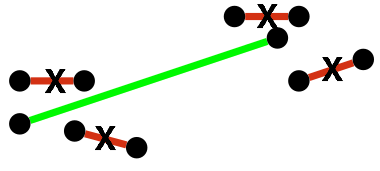
\includegraphics[scale=0.4]{imagenes/c3/Inform/Inform} 
	\caption[Ejemplo de conjunto de restricciones informativo.]{Ejemplo de conjunto de restricciones informativo. \cite{Survey:2007}}\label{fig:figure16}
\end{figure}


La informatividad se estima utilizando el conjunto de restricciones como un conjunto de test, de manera que se mide la habilidad del algoritmo para predecir las restricciones presentes en él. Formalizando, dado un conjunto de restricciones $R$ y un algoritmo $A$, obtenemos la partición $P_A$ aplicando el algoritmo al conjunto de datos de entrada especificando el conjunto de restricciones vacío. Calculamos entonces la fracción de las restricciones incumplidas por $P_A$ \cite{Survey:2007}:

\begin{equation}
I_A(R) = \frac{1}{|R|}\left[ \sum_{r \in R} unsat(r, P_A) \right] 
\end{equation}

\clearpage

Por otra parte, la \textbf{coherencia} mide el grado de concordancia dentro del propio conjunto de restricciones respecto a una métrica dada ($D$). Por ejemplo, la Figura \ref{fig:figure17} muestra dos restricciones paralelas y muy cercanas, pero de distinto tipo. Es en casos como este en los que se da una contradicción, ya que las restricciones \acf{ML} indican que la distancia entre las instancias involucradas en ellas es pequeña, mientras que las de tipo \acf{CL} deben indicar lo contrario.

\begin{figure}[!h]
	\centering
	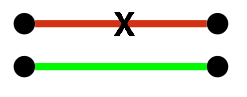
\includegraphics[scale=0.4]{imagenes/c3/Coherencia/Coher1}
	\caption[Ejemplo de conjunto de restricciones contradictorio.]{Ejemplo de conjunto de restricciones contradictorio. \cite{Survey:2007}}\label{fig:figure17}
\end{figure}

Entonces, la medida de coherencia viene dada por el grado de solapamiento que presentan las restricciones al interpretarlas como vectores en el espacio y proyectarlas sobre uno de los ejes, tal y como se muestra en la Figura \ref{fig:figure18}.

\begin{figure}[!h]
	\centering
	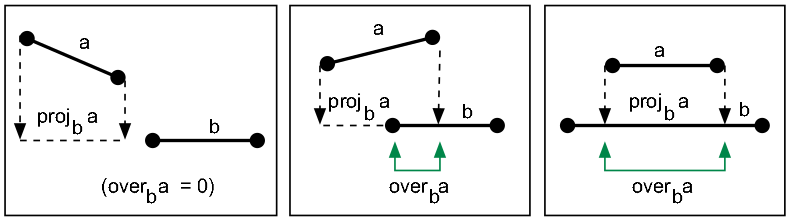
\includegraphics[scale=0.4]{imagenes/c3/Coherencia/Coher2}
	\caption[Representación de la medida de coherencia.]{Representación de la medida de coherencia. \cite{Survey:2007}}\label{fig:figure18}
\end{figure}

\section{Resumen}

El clustering con restricciones incorpora nueva información al problema del clustering original, esta viene dada en forma de especificaciones de pertenencia al mismo o a diferentes clusters sobre parejas de instancias. Las restricciones, ya sean \acf{ML}, \acf{CL}, o restricciones de distancia, son utilizadas para guiar al método de clustering que apliquemos al conjunto de datos en cuestión, en la búsqueda de la partición resultado.

Los método de clustering derivados de este concepto han demostrado ser de gran utilidad en múltiples ámbitos, así como presenta problemas que pueden ser subsanados estudiando en profundidad las restricciones a emplear para resolver cada problema.



































\chapter{Algoritmos de clustering con restricciones}\label{ch:Algoritmos}

Una vez introducido el problema del clustering con restricciones, pasamos a profundizar en los métodos para su aplicación. Este capítulo presenta 5 algoritmos de clustering con restricciones, cuyos resultados serán expuestos más tarde, en el Capítulo \ref{ch:Experimentación}.

\section{Formalización del problema}

Definido ya el problema del clustering con restricciones en el Capítulo \ref{ch:Clustering con restricciones}, especificamos la manera de notar sus elementos, de forma que sea sencillo referirse a ellos.

\begin{itemize}
	
	\item Notaremos con $X$ a la matriz de $n\times p$ que contiene el conjunto de datos de entrada.
	
	\item Notaremos con $x_i \;\; t.q. \;\; i \in \{1, \cdots, n\}$ a cada instancia de $X$, por lo que $x_i$ es un vector en el espacio $\mathbb{R}^p$ ($x_i \in \mathbb{R}^p$).
	
	\item Notaremos con $R$ al conjunto de restricciones, tanto las de tipo \acs{ML} como las \acs{CL}, es decir $R = ML \cup CL$. 
	
	\item Notaremos con $K$ el número de clusters de la partición resultante.
	
	\item Notaremos con $C$ el conjunto de clusters, y con $c_i \; t.q. \; i \in \{1, \cdots, K\}$ a cada uno de ellos, por tanto $C = \{c_i, \cdots, c_K\}$.
	
	\item Notaremos con $V$ la matriz de $K\times p$ que almacena el conjunto de centroides asociados a los clusters, de manera que $v_i \in \mathbb{R}^p$ corresponde al cluster $c_i$.
	
\end{itemize}
Cabe destacar que los elementos y parámetros particulares de cada algoritmo serán definidos en la sección correspondiente al mismo, así como que no todos los elementos expuestos anteriormente son comunes a todos los algoritmos; si bien sí que lo son a la mayoría de ellos.

\section{Constrained K-means} \label{copkm}

El algoritmo K-medias (\acs{KM}, Apéndice \ref{ap:kmeans}) es uno de los más básicos para aplicar clustering. Así, el algoritmo COP-K-medias (\textit{COP-K-means}) es la adaptación inmediata de \acs{KM} al clustering con restricciones. Para realizar un estudio detallado sobre el mismo tomaremos como base el trabajo de Wagstaff et al. (2001) \cite{Wagstaff:2001b}.

El cambio más notable que supone COP-K-medias respecto al tradicional K-medias, consiste en modificar la regla de asignación de instancias a clusters de este último, para comprobar que dicha asignación no viola ninguna restricción. De esta manera, en cada iteración se intenta asignar cada instancia $x_i$ al cluster más cercano $c_j$. Esta asignación sólo se llevará a cabo si, como hemos dicho, no se viola ninguna restricción. Si existe una instancia $x_{ML}$ que debe ser asignada al mismo cluster que $x_i$, pero ya ha sido incluida en otro cluster, o existe una instancia $x_{CL}$ en $c_j$ que no puede ser agrupada junto a $x_i$, entonces $x_i$ no puede ser asignado a $c_j$. El proceso continúa hasta encontrar una asignación legal para $x_i$, en caso de que no se encuentre se devuelve la partición vacía como resultado. Así el algoritmo proporciona una partición de $X$ que cumple necesariamente todas las restricciones especificadas en $R$. El Algoritmo \ref{alg:ckm} corresponde al pseudocódigo asociado a COP-K-medias \cite{Wagstaff:2001b}:


\begin{algorithm}
	
	\BlankLine
	\KwIn{Conjunto de datos $X$, conjunto de restricciones $R$, número de clusters $K$.}
	\KwOut{Partición $P$ del conjunto de datos $X$.}
	\BlankLine
	\textbf{función} COPKM($X$, $R$, $K$) \Begin{
		\BlankLine
		1. Sean $V = \{v_1,\cdots ,v_K\}$ los centroides iniciales\\
		2. Asignar cada instancia $x_i \in X$, al cluster $c_j$ asociado al centroide más cercano $v_j$ tal que ViolaRestriccion($x_i$, $c_j$, $R$) = falso. Si no existe $c \in C \;\;\; t.q.$ ViolaRestriccion($x_i$, $c_j$, $R$) = falso, \KwRet $\emptyset$.\\
		3. Para cada cluster $c_i$, actualizar su centroide $v_i$ realizando un promedio de todas las instancias $x_i$ asignadas a él.\\
		4. Iterar entre (1.) y (2.) hasta converger.\\
		5. \KwRet $C$
		\BlankLine
	}
	\BlankLine
	\KwIn{Instancia $x$, cluster $c$, conjunto de restricciones $R$}
	\BlankLine
	\textbf{función} ViolaRestriccion($x$, $c$, $R$) \Begin{
		\BlankLine
		1. Para cada $(x, x_{ML}) \in ML$, si $x_{ML} \notin R$ \KwRet \textbf{true}.\\
		2. Para cada $(x, x_{CL}) \in CL$, si $x_{CL} \notin R$ \KwRet \textbf{true}.\\
		3. En otro caso, \KwRet \textbf{false}.
		\BlankLine
	}
	
	\caption{COP-K-medias}\label{alg:ckm}
\end{algorithm}

Existen multitud de criterios de convergencia estandarizados, aunque es común emplear uno adaptado al problema particular que queramos solucionar. El más extendido consiste en calcular la diferencia de la posición de los centroides entre dos iteraciones sucesivas, de forma que cuando ésta sea menor que un umbral dado detenemos el proceso de iteración.

\section{Constrained Evidential K-means} \label{cekm}

Tal y como indican Violaine et al. (2012) \cite{CECM:2012}, cuyo trabajo es el fundamento de la siguiente sección, para comprender el algoritmo  \acf{CEKM}, primero es necesario realizar una introducción al algoritmo K-medias difuso (\textit{Fuzzy K-means}, \acs{FKM}). En él, cada instancia puede pertenecer a uno o más clusters, con diferentes grados de pertenencia. La matriz que almacena esta información, es decir, la partición difusa, se nota con $U$, y se calcula minimizando la siguiente función:

\begin{equation}
\sum_{j=1}^{K} u_{ij} \;\; t.q. \;\; u_{ij} \in [0,1] \forall i,j
\label{eqn2}
\end{equation}

Donde $u_{ij}$ representa el grado de pertenencia de la instancia $i$ al cluster $j$, y $K$ es el número de clusters. Sin embargo, este método puede producir resultados contraintuitivos cuando los datos a los que se aplica son ruidosos o presentan instancias aisladas (\textit{outliers}).

El clustering evidencial (\textit{evidential clustering}) da solución a los problemas que presenta el algoritmo \acs{FKM}, introduciendo el concepto de partición de creencia (\textit{credal partition}), que extiende los conceptos existentes de particiones fuertes, difusas y probabilísticas. De esta forma, en una partición de creencia, se asigna a cada instancia una masa de creencia (\textit{mass of belief}), no sólo para un único cluster, sino para cualquier conjunto de los mismos. El método \acs{CEKM} combina las ventajas del uso de las restricciones con las del uso de funciones de creencia.

\subsection{Funciones de creencia}

La teoría de la evidencia de Dempster-Shafer ofrece un marco teórico para trabajar con información parcial y no completamente fiable; tomamos de ella los conceptos relativos a las funciones de creencia.

Consideremos la variable $c$ que toma valores en el conjunto finito $C = \{c_1 \cdots c_K \}$. El conocimiento parcial sujeto al valor real que adopta $c$ puede ser representado mediante una función de masa $m$, que es una aplicación de $C$ al intervalo $[0,1]$:

\begin{equation}
\sum_{A \subseteq C} m(A) = 1
\label{eqn3}
\end{equation}

A los subconjuntos $A$ de $C$ que cumplen que $m(A) > 0$ se los denomina conjuntos focales (\textit{focal sets}) de $m$. El valor del conjunto focal $m(A)$ se interpreta como la fracción de una unidad de masa de creencia que está asignada a $A$ y que no puede ser asignada a ningún otro subconjunto de $A$. Si el único conjunto focal es $C$, nos encontramos en el caso de completa ignorancia sobre los datos. Por el contrario, si la masa de creencia se asigna a un único elemento de $C$, estaríamos en el caso de certeza absoluta.

Se dice que una función de masa $m$ está normalizada si $m(\emptyset) = 0$. Sin embargo, bajo la hipótesis de mundo abierto, una función de masa en la que $m(\emptyset) > 0$ se interpreta como la cantidad de creencia que se le asigna a la hipótesis de que el verdadero valor de $c$ puede no encontrarse en $C$.

Dada una función de masa $m$, podemos definir una función de plausibilidad $pl:2^C \rightarrow [0,1]$ y una función de creencia $bel: 2^C \rightarrow [0,1]$ de la siguiente manera:

\begin{equation}
pl(A) = \sum_{B \cap A \neq \emptyset} m(B) \;\;\; \forall A \subseteq C
\label{eqn4}
\end{equation}

y 

\begin{equation}
bel(A) = \sum_{B \subseteq A, B \neq \emptyset} m(B) \;\;\; \forall A \subseteq C
\label{eqn5}
\end{equation}

De esta forma, las funciones $pl$ y $bel$ están relacionadas como sigue:

\begin{equation}
pl(A) = 1 - m(\emptyset) - bel(\bar{A})
\label{eqn6}
\end{equation}

Donde $\bar{A}$ representa el complemento de $A$.  La cantidad $bel(A)$ se interpreta como el grado de creencia en $A$, tomando en consideración la masa de creencia asignada a $A$ y a los subconjuntos no vacíos de $A$. Por el contrario, $pl(A)$ mide hasta qué punto es erróneo no creer en $\bar{A}$.

Con el objetivo de tomar decisiones en base al valor de $c$, es posible transformar la función de masa en una distribución de probabilidad pignística, definida, para una función de masa normalizada, como:

\begin{equation}
BetP(c) = \sum_{c \in A} \frac{m(A)}{|A|} \;\;\; \forall c \in C
\label{eqn7}
\end{equation}

\subsection{FKM (fuzzy K-means) y sus variantes}

Cada cluster $c_j \in C$ con $j \in \{1,\cdots,K\}$ está representado por un vector $v_j \in \mathbb{R}^p$, esto es, un centroide. Además, definimos $V$ como la matriz compuesta por todos los centroides, y $U = (u_{ij})$ como la partición difusa que contiene los grados de pertenencia de cada instancia de $X$ a cada cluster. El algoritmo \acf{FKM} calcula las matrices $U$ y $V$ de manera que minimiza (sujeto a las Ecuaciones \ref{eqn2} y \ref{eqn3}) la siguiente función:

\begin{equation}
J_{FKM}(U,V) = \sum_{i=1}^{n}\sum_{j=i}^{K} u_{ij}^\beta d_{ij}^2
\label{eqn8}
\end{equation}

Donde $d_{ij}$ representa la distancia Euclídea entre el objeto $x_i$ y el centroide $v_j$, y donde $\beta > 1$ es el exponente que controla el grado de difusión de la partición. La función objetivo se minimiza mediante un algoritmo iterativo que optimiza los centroides y los grados de pertenencia de manera alterna. El algoritmo empieza con una asignación inicial sobre la que realiza modificaciones hasta que converge.

Para detectar datos ruidosos u outliers empleamos el algoritmo \acf{NC}. Este método consiste en añadir a los $K$ clusters iniciales uno adicional llamado ``cluster ruidoso'', asociado a una distancia fija $\rho$ respecto a todos los objetos. El parámetro $\rho$ controla la cantidad de datos que serán considerados como outliers. La pertenencia $u_{i*}$ de un objeto $i$ al cluster ruidoso se calcula como:

\begin{equation}
u_{i*} = 1 - \sum_{j=1}^{K} u_{i,j} \;\;\; i = 1,n
\label{eqn9}
\end{equation}

Por tanto, la función objetivo que minimiza el algoritmo \acs{NC} no es más que una combinación del cálculo de pertenencia de objetos al cluster ruidoso y de la que minimizaba el algoritmo \acs{FKM}:

\begin{equation}
J_{NC}(U,V) = \sum_{i=1}^{n}\sum_{j=i}^{K} u_{ij}^\beta d_{ij}^2 + \sum_{i=n}^{K} \rho^2 u_{i*}^\beta
\label{eqn10}
\end{equation}

\subsection{El algoritmo EKM (Evidential K-means)}

Es posible obtener una versión credibilística del algoritmo \acs{NC} reemplazando la matriz asociada a la partición difusa $U$ con una partición de creencia, que notaremos con $M$. En este contexto, el conocimiento parcial asociado a la pertenencia de un objeto a una clase viene representado por una función de masa aplicada al conjunto $C$ de posibles clases. Por tanto, la masa de creencia puede ser asignada a cualquier subconjunto $A$ de $C$, y no sólo a elementos únicos de $C$. Este esquema hace posible modelar una amplia variedad de circunstancias, que van de la completa ignorancia sobre el conjunto de datos hasta la completa certeza sobre el mismo.

Para ilustrar estas ideas se propone el siguiente ejemplo: consideramos un conjunto de cuatro objetos que deben ser clasificados en dos clases. La Tabla \ref{tab:tabla2} contiene la partición de creencia asociada a estos datos. La clase del primer objeto es conocida con certeza, ya que su masa de creencia está asignada a un solo elemento de $C$. Por el contrario, la clase del segundo objeto es completamente desconocida. La masa de creencia del tercer objeto está repartida entre dos elementos de $C$. Por tanto, tenemos conocimiento probabilístico sobre la clase a la que pertenece. El último objeto representa un outlier, ya que su masa de creencia está asignada al conjunto vacío.

\begin{table}[h]
	\centering
	\setlength{\arrayrulewidth}{1mm}
	\setlength{\tabcolsep}{10pt}
	\renewcommand{\arraystretch}{1}
	
	\rowcolors{2}{gray!25}{white}
	\begin{tabular}{ >{\centering\arraybackslash}m{1cm}  >{\centering\arraybackslash}m{1cm}>{\centering\arraybackslash}m{1cm}>{\centering\arraybackslash}m{1cm}>{\centering\arraybackslash}m{1cm}}
		\hline
		\rowcolor{black}
		\multicolumn{5}{c}{\bf \color{white}{Ejemplo de partición de creencia}}\\
		\hline
		\rowcolor{gray!50}
		\textbf{$A$} & \textbf{$m_1(A)$} & \textbf{$m_2(A)$} & \textbf{$m_3(A)$} & \textbf{$m_4(A)$} \\
		$\emptyset$ & $0$ & $0$ & $0$ & $1$ \\
		$\{c_1\}$ & $1$ & $0$ & $0.3$ & $0$ \\
		$\{c_2\}$ & $0$ & $0$ & $0.7$ & $0$ \\
		$C$ & $0$ & $1$ & $0$ & $0$ \\
		\hline
		
	\end{tabular}
	\caption[Ejemplo de partición de creencia]{Ejemplo de partición de creencia \cite{CECM:2012}}
	\label{tab:tabla2}
\end{table}

\acf{EKM} es uno de los algoritmos que opera con una partición de creencia obtenida en base a los datos. Si tomamos $m_{ij}$ como el grado de creencia de que el objeto $x_i$ pertenece al subconjunto $A_j \subseteq C$, obtener una partición de creencia implica determinar, para cada $x_i$, las cantidades $m_{ij} = m_i(A_j)\;\; \forall A_j \neq \emptyset, A_j \subseteq C$. De esta manera, cuando la distancia $d_{ij}$ entre $x_i$ y $A_j$ es alta (baja), $m_{ij}$ será un valor bajo (alto).

Tal y como sucedía en \acf{FKM}, cada clase $c_l$ está representada por un centroide $v_l \in \mathbb{R}^p$. Entonces, para cada subconjunto $A_j$ de $C$ distinto de $\emptyset$ se calcula su centroide $\bar{v}_j$ como el baricentro de los centros asociados a las clases presentes en $A_j$:

\begin{equation}
\bar{v}_j = \frac{1}{|A_j|} \sum_{l=1}^{K} S_{lj} v_l
\label{eqn11}
\end{equation}

donde el valor $S_{lj}$ viene definido por:

\begin{equation}
S_{lj} = \begin{cases}
1 \;\;\; \textbf{si} \;\;\; c_l \in A_j\\
0 \;\;\; \textbf{otro caso}
\end{cases}
\label{eqn12}
\end{equation}

La distancia $d_{ij}$ entre la instancia $x_i$ y el conjunto focal $A_j$ se calcula como:

\begin{equation}
d_{ij} = ||x_i - \bar{v}_j||
\label{eqn13}
\end{equation}

Entonces, el algoritmo \acs{EKM} calcula las matrices $M$ y $V$ tratando de minimizar un criterio similar al del algoritmo \acs{NC}:

\begin{equation}
J_{EKM}(M,V) = \frac{1}{2^cn} \sum_{i=1}^{n}\sum_{A_j \neq \emptyset} |A_j|^\alpha m_{ij}^\beta d_{ij}^2 + \sum_{i=1}^{n} \rho^2 m_{i\emptyset}^\beta
\label{eqn14}
\end{equation}

sujeto a las restricciones $m_{ij} \ge 0 \;\; \forall i,j$, y $m_{i\emptyset} \ge 0 \;\; \forall i$, y:

\begin{equation}
\sum_{j/A_j \subseteq C, A_j \neq \emptyset} m_{ij} + m_{i\emptyset} = 1 \;\;\; \forall i = 1,n
\label{eqn15}
\end{equation}

Donde $m_{i\emptyset}$ denota la cantidad de masa de creencia de la instancia $x_i$ asignada al conjunto vacío. El parámetro $\rho$ representa la distancia de cualquier objeto al conjunto vacío, y el parámetro $\alpha$ se introduce para controlar la penalización por asignar objetos a conjuntos con alta cardinalidad.

Gracias a la restricción expuesta en la Ecuación \ref{eqn15}, podemos obtener equivalencia entre los algoritmos \acs{NC} y \acs{EKM}. El algoritmo \acs{EKM} asigna una gran masa de creencia al conjunto vacío para un objeto dado cuando éste se encuentra lejos de todos los subconjuntos $A_j$.

Como en \acs{FKM} y \acs{NC}, la partición de creencia se calcula aplicando un proceso de optimización iterativo, que actualiza las masas  y los centroides de forma alterna. La regla de optimización de $M$ es muy similar a su homóloga en \acs{NC}, excepto por el número de valores $m_{ij}$ a calcular, que en este caso es $2^c$, en lugar de los $K + 1$ grados de pertenencia que eran necesarios en \acs{NC}. De esta manera, la función de masa queda definida como:

 \begin{equation}
m_{ij} = \frac{|A_j|^{-\alpha/(\beta-1)} d_{ij}^{-2/(\beta-1)}}{\sum_{A_l \ne \emptyset}|A_l|^{-\alpha/(\beta-1)} d_{ij}^{-2/(\beta-1)} + \rho^{-2/(\beta-1)}}
 \label{eqn16}
 \end{equation}
 
 y
 
\begin{equation}
m_{i\emptyset} = 1 - \sum_{A_j \ne \emptyset}m_{ij} \;\;\; i = 1,n
\label{eqn17}
\end{equation}

Por otra parte, la regla de actualización de los centroides resulta un poco más compleja. Requiere resolver un sistema de ecuaciones lineal en cada paso del proceso, en el que cada columna de $V$ es la solución para un sistema lineal de $K$ ecuaciones y $K$ incógnitas. Tomamos $B$ como la matriz de tamaño $(K \times p)$ definida por:

\begin{equation}
B_{lq} = \sum_{i=1}^{n} X_{iq} \sum_{A_j \ni c_l} |A_j|^{\alpha-1} m_{ij}^\beta \;\;\; l = 1,K \;\;\; q =1,p
\label{eqn18}
\end{equation}

y la matriz $H$ de tamaño $(K \times K)$ como:

\begin{equation}
H_{lt} = \sum_{i} \sum_{A_j \supseteq \{c_t,c_l\}} |A_j|^{\alpha - 2} m_{ij}^\beta \;\;\; t,l = 1,K
\label{eqn20}
\end{equation}

de forma que $V$ es la solución del sistema de ecuaciones lineal $H\times V = B$, que puede ser resuelto mediante técnicas estándar. El proceso de cálculo que deriva en estas ecuaciones viene detallado en el trabajo de Violaine et al. (2012). \cite{CECM:2012}

\subsection{Incorporación de restricciones a EKM}

Una vez definidos los elementos que conforman el algoritmo \acs{EKM}, debemos incorporar las restricciones a nivel de instancia al marco de las funciones de creencia, para integrarlas en el cálculo de la partición de creencia.

Siendo $x_i$ y $x_j$ dos instancias, podemos calcular la función de masa conjunta en el producto cartesiano $C \times C = C^2$ conociendo sus funciones de masa particulares $m_i$ y $m_j$:

\begin{equation}
\begin{split}
m_{i \times j}(A \times B) &= m_i(A)m_j(B) \;\;\; A,B \subseteq C, A \neq \emptyset, B \neq \emptyset\\
m_{i \times j}(\emptyset) & = m_i(\emptyset) + m_j(\emptyset) - m_i(\emptyset)m_j(\emptyset)
\end{split}
\label{eqn21}
\end{equation}

Conociendo $ m_{i \times j} $ es posible calcular la plausibilidad asociada a que los objetos $x_i$ y $x_j$ pertenezcan a la misma clase que, en el espacio $C^2$, corresponde al subconjunto $\theta = \{(c_1, c_1), (c_2, c_2), \cdots, (c_K, c_K)\}$. El caso contrario corresponde al complemento de $\theta$, es decir, $\bar{\theta}$:

\begin{equation}
\begin{split}
pl_{i\times j}(\theta) &= \sum_{A \cap B \ne \emptyset}m_i(A)m_j(B)\\
pl_{i\times j}(\bar{\theta}) &= 1 - m_{i\times j}(\emptyset) - \sum_{l=1}^{K} m_i(\{c_l\})m_j(\{c_l\})
\end{split}
\label{eqn23}
\end{equation}

Los cálculos y simplificaciones de los que se obtienen estas ecuaciones se encuentran en el trabajo de Violaine et al. (2012). \cite{CECM:2012}

\subsection{Función objetivo de CEKM}

Asumimos ahora que la partición de creencia es desconocida, y que disponemos del conjunto de restricciones. En tal caso será necesario buscar una partición de creencia que considere las similitudes y diferencias obtenidas en base a los datos y a las restricciones. Para ello debemos buscar que $pl_{i\times j} (\theta)$ sea tan bajo como sea posible si $(x_i, x_i) \in CL$, así como que $pl_{i\times j} (\bar{\theta})$ también lo sea si $(x_i, x_i) \in ML$. A tal fin, integramos una penalización en el criterio de optimización de \acs{EKM} de la siguiente manera:

\begin{equation}
J_{CONST} = \frac{1}{|R|} \left[\sum_{(x_i,x_j) \in ML} pl_{i\times j} (\bar{\theta})\;\; + \sum_{(x_i,x_j) \in CL} pl_{i\times j} (\theta)\right]
\label{eqn25}
\end{equation}

De esta forma, la función objetivo a minimizar pasa a ser:

\begin{equation}
J_{CEKM}(M,V) = (1- \xi)J_{EKM}(M,V) + \xi J_{CONST}
\label{eqn26}
\end{equation}

donde el parámetro $\xi \in [0,1]$ se utiliza para controlar el compromiso entre las restricciones y el modelo geométrico asociado a la métrica de distancia.

\subsection{Proceso de optimización de CEKM}

De igual forma que en \acs{FKM}, \acs{NC} y \acs{EKM}, el modelo de optimización de \acs{CEKM} consiste en actualizar $M$ y $V$ de forma alterna. Cabe destacar que el término de penalización añadido a \acs{CEKM} no depende de los centroides de los clusters, y por tanto se puede aplicar el mismo modelo de actualización que en \acs{EKM} (Ecuaciones \ref{eqn18} y \ref{eqn20}). Generalmente el problema es mucho más complejo para las masas de creencia. Sin embargo, fijando $\beta = 2$, la Ecuación \ref{eqn26}, que describe la función objetivo, pasa a ser cuadrática respecto a $m_{ij}$. Con esto, y como las restricciones son lineales, se pueden emplear algoritmos de programación cuadrática para resolver el problema de la actualización de las masas de creencia. El proceso de cálculo asociado a \acs{CEKM} queda resumido en el Algoritmo \ref{alg:cecm}. 


\begin{algorithm}
	
	\BlankLine
	\KwIn{Conjunto de datos $X$, conjunto de restricciones $R$, número de clusters resultantes $K$, los parámetros $\alpha$, $\rho$ y $\xi$.}
	\KwOut{Partición de creencia $M$, centroides $V$.}
	\BlankLine
	\textbf{función} CEKM($X$, $R$, $K$, $\alpha$, $\rho$, $\xi$) \Begin{
		\BlankLine
		1. Sean $V = \{v_1,\cdots ,v_K\}$ los centroides iniciales.\\
		2. Actualizar las masas ($M$) resolviendo el problema de programación cuadrática definido por \ref{eqn26} sujeto a \ref{eqn15}\\
		3. Actualizar los centroides ($V$) resolviendo el sistema de ecuaciones lineal definido por \ref{eqn18} y \ref{eqn20} con $\beta = 2$\\
		4. Iterar entre (2.) y (3.) hasta que no haya cambios significativos en $V$.\\
		5. \KwRet $M$, $V$
		\BlankLine
	}
	\caption{\acf{CEKM}}
	\label{alg:cecm}
\end{algorithm}

En la mayoría de las ocasiones se requiere como resultado de un algoritmo de clustering una partición fuerte del conjunto de datos, y no una partición de creencia. Podemos obtener una partición difusa calculando la probabilidad pignística $BetP_i(\{c_j\})$ en base a cada función de masa $m_i$ aplicando la Ecuación \ref{eqn7}, e interpretar este valor como el grado de pertenencia del objeto $i$ al cluster $j$. Una vez obtenida la partición difusa, podemos procesarla como precise el problema para obtener la partición fuerte. La manera más común de hacerlo es asignar cada instancia al cluster para el que presente un mayor grado de pertenencia.

Otra manera de extraer información de la partición de creencia es asignar cada objeto al subconjunto de clases que contengan un mayor porcentaje de su masa de creencia. De esta forma obtenemos una partición de creencia fuerte de, como mucho, $2^K$ clusters. A partir de esta partición es posible discernir qué objetos deben ser asignados a un único cluster sin ambigüedad, además de detectar aquellos que se encuentran en la frontera de dos o más clusters, que a menudo suelen ser relevantes.

\clearpage

\section{Linear Constrained Vector Quantization Error} \label{lcvqe}

Tomando como base el trabajo de Pelleg y Dorit (2007) \cite{LCVQE:2007}, es necesario realizar una introducción al algoritmo \acf{CVQE} antes de detallar el algoritmo \acs{LCVQE}, puesto que este último consiste en una modificación sobre el primero para mejorar, principalmente, su orden de complejidad.

\subsection{El algoritmo CVQE}

El algoritmo \acs{CVQE} consiste en una generalización del algoritmo K-medias (\acs{KM}, Apéndice \ref{ap:kmeans}) para incluir las restricciones. En el algoritmo \acs{KM} los centroides $v_i$ se actualizan en cada iteración siguiendo la regla:

\begin{equation}
v_i = \frac{1}{|c_i|} \sum_{x_i \in c_i} x_i
\label{eqn27}
\end{equation}

que no es más que un promedio de todas las instancias asignadas al cluster asociado al centroide $v_i$. Tras la actualización, se recalculan las asignaciones de forma que cada instancia esté asociada al cluster más cercano. Esto deriva en una regla que minimiza la función \acf{VQE}:

\begin{equation}
VQE = \frac{1}{2} \sum_{j = i}^{K} \sum_{x_i \in c_i} (v_j - x_i)^2
\label{eqn28}
\end{equation}

\acs{CVQE} modifica la función \acs{VQE}, añadiendo a la misma un término de penalización que considera las restricciones incumplidas. Por simplicidad, notaremos el cardinal de $ML$ con $ml$, así como el de $CL$ con $cl$, y definiremos el conjunto de restricciones $R$ como una lista de parejas de instancias: 

\begin{equation}
\{(x_1(i), x_2(i))\}_{i=1}^{ml+cl}
\label{eqn29}
\end{equation}

Además definimos $M$ como la función que, dada una instancia, devuelve el índice del cluster que la contiene: $M = \{j | x \in c_j\}$, y las funciones $g(i) = M(x_1(i))$ y $g^\prime(i) = M(x_2(i))$. Por otra parte, definimos $h(i)$ como la función que devuelve el centroide más cercano al centroide $v_i$. Finalmente definimos $vl(i)$ de manera que indica si las restricción i-ésima ha sido violada, por tanto, para $i = 1, \cdots , ml \;\; vl(i) = 1 \leftrightarrow g(i) \neq g^\prime(i)$, de forma similar $i = ml + 1, \cdots , ml + cl \;\; vl(i) = 1 \leftrightarrow g(i) = g^\prime(i)$. Definidas estas funciones, la regla de actualización de \acs{CVQE} es:

\begin{equation}
v_j = \frac{1}{N_j} \left[ \sum_{x_i \in c_i}x_i + 
\sum_{l=1,g(l) = j}^{ml} vl(l) v_{g^\prime(l)} + 
\sum_{l=ml + 1,g(l) = j}^{ml + cl} vl(l) v_{h(g^\prime(l))}
\right]
\label{eqn30}
\end{equation}

donde $N_j$ viene definido por: 

\begin{equation}
N_j = |c_j| + \sum_{l=1,g(l) = j}^{ml + cl} vl(l)
\label{eqn31}
\end{equation}

De manera intuitiva, para las restricciones $ML$ incumplidas, uno de los dos centroides afectados se mueve hacia el otro, mientras que para las $CL$ incumplidas se mueve una de las instancias hacia el siguiente centroide más cercano a su cluster. De forma similar a \acs{KM}, cada instancia se reasigna después de cada iteración para minimizar la función de error $CVQE = \sum_{j=i}^{K} CVQE_j$, donde $CVQE_j$ es:

\begin{equation}
CVQE_j = \frac{1}{2} \sum_{x_i \in c_j} T_{j,1} + 
\frac{1}{2} \sum_{l=1,g(l) = j}^{ml} T_{j,2} + 
\frac{1}{2} \sum_{l=ml + 1,g(l) = j}^{ml + cl} T_{j,3}
\label{eqn32}
\end{equation}

y los términos $T_{j,1}$, $T_{j,2}$ y $T_{j,3}$ vienen definidos como: 

\begin{equation}
\begin{split}
T_{j,1} &= (v_j - x_i)^2\\
T_{j,2} &= \left[ (v_j - v_{g^\prime(l)})^2 \cdot vl(l) \right]\\
T_{j,3} &= \left[ (v_j - v_{h(g^\prime(l))})^2 \cdot vl(l) \right]
\end{split}
\label{eqn33}
\end{equation}

Cabe destacar que, al contrario de lo que sucede en \acf{KM}, en \acs{CVQE}, un cluster $c_i$ puede contener instancias para las que el centroide $v_i$ no es el más cercano a ella.

En cada paso, el algoritmo \acs{CVQE} asigna cada par de instancias implicadas en una restricción de manera que se minimiza la función $CVQE$.

A continuación se exponen algunas de las características del algoritmo \acs{CVQE} que resultan relevantes para la compresión de \acs{LCVQE}.

En primer lugar, el orden en el que se especifican las instancias implicadas en las restricciones es relevante. Consideremos una restricción formada por las instancias $(x_i(l), x_2(l))$, de forma que $x_1(l) \in c_{g(l)}$, y $x_2(l) \in c_{g^\prime(l)}$. Sólo $c_{g(l)}$ se ve afectado por violar la restricción, mientras que sobre $c_{g^\prime(l)}$ no se aplica ningún cambio. Esta regla se cumple tanto para las restricciones \acf{ML} como para las \acf{CL}.

\begin{observacion}
	
	En \acs{CVQE} el orden en el que se especifican las instancias implicadas en una restricción es relevante.
	
\end{observacion}

En segundo lugar, determinar la asignación que minimiza la función de error requiere $\mathcal{O}(K^2)$ cálculos para cada restricción. Por tanto, el método puede resultar computacionalmente pesado para grandes conjuntos de restricciones o clusters. Además, no es posible descartar ninguna opción de los cálculos aparte de las triviales.

\begin{observacion}
	
	El método \acs{CVQE} es computacionalmente pesado para grandes conjuntos de datos o restricciones.
	
\end{observacion}

Para ejemplificar esto consideramos la Figura \ref{fig:figure19}. En ella, el par $(x,y)$ es una restricción \acs{ML}, y los centroides existentes son $\{v_1,\cdots,v_6\}$. Dependiendo de los valores $R$, $\delta$ y $\epsilon$ las instancias pueden ser asignadas a los centroides $(v_1, v_2)$, $(v_3, v_4)$, $(v_5, v_6)$. Por tanto, las $K^2$ opciones deben ser consideradas para cada restricción al decidir una asignación.

\begin{figure}[!h]
	\centering
	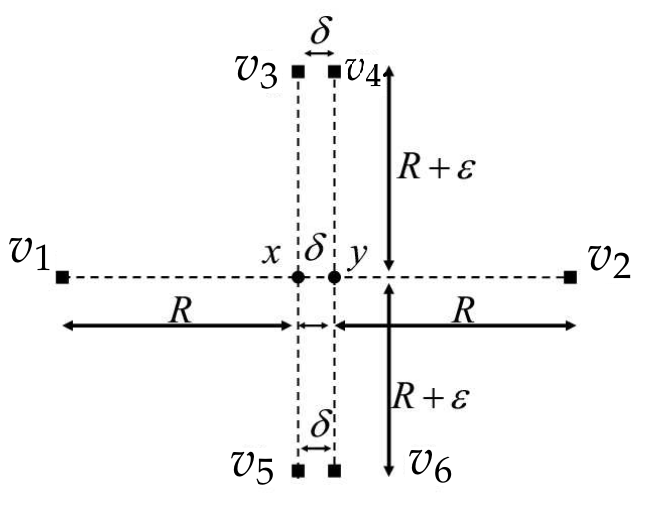
\includegraphics[scale=0.4]{imagenes/c4/Fig1}
	\caption[Ejemplo de CVQE.]{Ejemplo de CVQE. \cite{LCVQE:2007}}\label{fig:figure19}
\end{figure}

La última observación que debemos hacer está relacionada con el hecho de que la penalización por violar restricciones depende de la distancia entre los centroides implicados en ella, pero no de la distancia entre las instancias. 

\begin{observacion}
	
	El término de penalización por violar restricciones de \acs{CVQE} sólo depende de la distancia entre los centroides implicados en la restricción.
	
\end{observacion}

Para mostrar el problema que esto supone tomamos la Figura \ref{fig:figure20}, en la que se presentan dos problemas de clustering. Para ambos, los centroides existentes son $v_1$ y $v_2$, mientras que un problema incluye la restricción $ML(x_1, y)$ y el otro $ML(x_2, y)$.


\begin{figure}[!h]
	\centering
	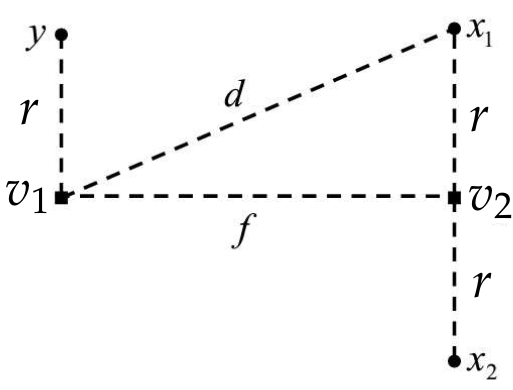
\includegraphics[scale=0.4]{imagenes/c4/Fig2}
	\caption[Ejemplo de CVQE.]{Ejemplo de CVQE. \cite{LCVQE:2007}}\label{fig:figure20}
\end{figure}

La Tabla \ref{tab:tabla3} recoge las asignaciones posibles en cada caso, así como el valor de la función $CVQE$. Vemos que, independientemente del valor de $d$ y $f$, ambos problemas tiene la misma solución, mientras que intuitivamente diríamos que violar la restricción $ML(x_1, y)$ debería acarrear una penalización mayor que violar $ML(x_2, y)$. Es más, en ambos casos la acción que aplica \acs{CVQE} es la misma, mover $v_1$ hacia $v_2$ en la recta que los une.

\begin{table}[!h]
	\centering
	\setlength{\arrayrulewidth}{1mm}
	\setlength{\tabcolsep}{10pt}
	\renewcommand{\arraystretch}{0.9}
	
	\rowcolors{2}{gray!25}{white}
	\begin{tabular}{ >{\centering\arraybackslash}m{2cm}  >{\centering\arraybackslash}m{2.5cm}>{\centering\arraybackslash}m{2cm}>{\centering\arraybackslash}m{2cm}}
		\hline
		\rowcolor{black}
		\multicolumn{4}{c}{\bf \color{white}{Valores de CVQE}}\\
		\hline
		\rowcolor{gray!50}
		\textbf{Restricción} & \textbf{$y \in c_1, x_i \in c_2$} & \textbf{$x_i,y \in c_1$} & \textbf{$x_i,y \in c_2$}  \\
		$ML(x_1, y)$ & $r^2 + r^2 + f^2$ & $r^2 + f^2 $ & $r^2 + d^2 $  \\
		$ML(x_2, y)$ & $r^2 + r^2 + f^2$ & $r^2 + f^2 $ & $r^2 + d^2 $  \\
		\hline
		
	\end{tabular}
	\caption[Valores de CVQE para el ejemplo]{Valores de CVQE para el ejemplo. \cite{CECM:2012}}
	\label{tab:tabla3}
\end{table}

\subsection{El algoritmo LCVQE}

El algoritmo \acs{LCVQE} minimiza una función similar a la que minimiza \acs{CVQE}. Con la diferencia de que, para cada asignación, \acs{LCVQE} considera, como mucho, los dos clusters más naturalmente apropiados para la asignación. Por ello, la complejidad del algoritmo es independiente de $K$, al contrario de lo que sucedía en \acs{CVQE}.

Intuitivamente, las restricciones \acs{ML} violadas modifican la actualización de los centroides para desplazarlos hacia la instancia opuesta. Para las restricciones \acs{CL} violadas, se determina cuál es la instancia más lejana al centroide común, sirviendo ésta como guía para mover el segundo centroide más cercano hacia ella. Con esto tenemos que, en \acs{LCVQE}, las restricciones son simétricas, es decir, no es relevante el orden en el que se especifiquen las instancias implicadas en ellas.

\begin{observacion}
	
	En \acs{LCVQE} las restricciones son simétricas, esto es, el orden en el que se especifiquen las instancias en ellas no es relevante.
	
\end{observacion}

Para formalizar la regla de actualización es necesario definir nuevas funciones. $L_j(i)$ devuelve la instancia de entre $x_1(i)$ y $x_2(i)$ que más lejos se encuentre del centroide $v_j$. $MM(x)$ devuelve el centroide más cercano a $x$ distinto de $v_{M(x)}$. Con esto la regla de actualización queda definida como:

\begin{equation}
v_j = \frac{1}{N_j} \left[ \sum_{x_i \in c_j} x_i + 
\frac{1}{2} S_1 + \frac{1}{2} S_2 + S_3 \right]
\label{eqn38}
\end{equation}

quedando los términos $S_1$, $S_2$ y $S_3$ definidos como sigue:

\begin{equation}
\begin{split}
S_1 &= \sum_{l=1,g(l) = j}^{ml} vl(l) \cdot x_2(l) \\
S_2 &= \sum_{l=1,g^\prime(l) = j}^{ml} vl(l) \cdot x_1(l) \\
S_3 &= \sum_{l=ml+1, j = MM(L_{M(x_1(l))}(l))}^{ml + cl} vl(l) \cdot L_{M(x_1(l))}(l)
\end{split}
\label{eqn80}
\end{equation}

donde $N_j$ en este caso se calcula como:

\begin{equation}
\begin{split}
N_j = & |c_j| + \frac{1}{2} \sum_{l=1,g(l) = j}^{ml} vl(l) + 
\frac{1}{2} \sum_{l=1,g^\prime (l) = j}^{ml} vl(l) + \\
& \sum_{l=ml+1,j = MM(L_{M(x_1(l))}(l))}^{ml + cl} vl(l)
\end{split}
\label{eqn41}
\end{equation}

Esta regla de actualización minimiza la función de error:

\begin{equation}
\begin{split}
E_j = & \frac{1}{2} \sum_{x_i \in c_j} T_{j,1} + 
\frac{1}{2} \sum_{l=1,g(l) = j}^{ml} T_{j,2} + 
\frac{1}{2} \sum_{l=ml + 1,g^\prime(l) = j}^{ml} T_{j,3} + \\
&\frac{1}{2} \sum_{l=ml+1,j = MM(L_{M(x_1(l))}(l))}^{ml + cl} T_{j,4}
\end{split}
\label{eqn42}
\end{equation}

quedando definidos los términos $T_{j,1}$, $T_{j,2}$, $T_{j,3}$ y $T_{j,4}$ como:

\begin{equation}
\begin{split}
T_{j,1} &= (v_j - x_i)^2\\
T_{j,2} &= \left[ \frac{1}{2} (v_j - x_2(l))^2 \cdot vl(l) \right]\\
T_{j,3} &= \left[ \frac{1}{2} (v_j - x_1(l))^2 \cdot vl(l) \right]\\
T_{j,4} &= \left[ (v_j - L_{M(x_1(l))}(l))^2 \cdot vl(l) \right]
\end{split}
\label{eqn43}
\end{equation}

El Algoritmo \ref{alg:lcvqe} recoge de manera resumida el proceso que sigue \acs{LCVQE} para obtener una partición de los datos. 

El criterio de convergencia puede estar basado en la diferencia de los centroides entre iteraciones sucesivas, así como en criterios de asignación de instancias a clusters o evaluaciones totales de la función de error.

El algoritmo \acs{LCVQE} requiere $\mathcal{O}(p)$ operaciones en cada paso, siendo $p$ el número de dimensiones, ya que sólo se consideran tres posibles asignaciones, independientemente del valor de $K$. Por tanto \acs{LCVQE} supera en eficiencia a \acs{CVQE}, que era altamente sensible al número de clusters y de restricciones.

\begin{observacion}
	
	El algoritmo \acs{LCVQE} es computacionalmente más eficiente que \acs{CVQE}, pues en cada paso realiza $\mathcal{O}(p)$ operaciones.
	
\end{observacion}

Finalmente, podemos estudiar como se comporta el algoritmo frente al ejemplo de la Figura \ref{fig:figure20}. La Tabla \ref{tab:tabla4} muestra las asignaciones posibles en cada caso, así como los valores \acs{LCVQE}. En ambos problemas asumimos que la asignación es $x_i \in c_2$ e $y \in c_1$. En el caso de la restricción $(x_1, y)$ el centroide se actualiza según la regla $c_1 = (y + \frac{1}{2}x_1)/1.5$, y en el caso de $(x_1, y)$ tenemos que $c_1 = (y + \frac{1}{2}x_2)/1.5$, resultados intuitivamente mejores que los que obteníamos con \acs{CVQE}, ya que el centroide se mueve hacia la distancia media de las instancias en lugar de hacia el otro centroide $c_2$.

\begin{observacion}
	
	El término de penalización por violar restricciones de \acs{CVQE} involucra las características espaciales de las instancias implicadas en ella.
	
\end{observacion}

\begin{table}[!h]
	\centering
	\setlength{\arrayrulewidth}{1mm}
	\setlength{\tabcolsep}{10pt}
	\renewcommand{\arraystretch}{1}
	
	\rowcolors{2}{gray!25}{white}
	\begin{tabular}{ >{\centering\arraybackslash}m{2cm}  >{\centering\arraybackslash}m{2.5cm}>{\centering\arraybackslash}m{2cm}>{\centering\arraybackslash}m{2cm}}
		\hline
		\rowcolor{black}
		\multicolumn{4}{c}{\bf \color{white}{Valores de LCVQE}}\\
		\hline
		\rowcolor{gray!50}
		\textbf{Restricción} & \textbf{$y \in c_1, x_i \in c_2$} & \textbf{$x_i,y \in c_1$} & \textbf{$x_i,y \in c_2$}  \\
		$ML(x_1, y)$ & $(d^2 + d^2)/2$ & $d^2$ & $d^2$  \\
		$ML(x_2, y)$  & $(d^2 + d^2)/2$ & $d^2$ & $d^2$ \\
		\hline
		
	\end{tabular}
	\caption[Valores de LCVQE para el ejemplo]{Valores de LCVQE para el ejemplo. \cite{CECM:2012}}
	\label{tab:tabla4}
\end{table}

\begin{algorithm}
	
	\BlankLine
	\KwIn{Conjunto de datos $X$, conjunto de restricciones $R$, centroides iniciales $V$, número de clusters $K$.}
	\KwOut{Partición $P$ del conjunto de datos $X$, centroides $V$.}
	\BlankLine
	\textbf{función} LCVQE($X$, $R$, $K$) \Begin{
		\BlankLine
		1. Inicialización de $GMLV_j = GCLV_j = \emptyset \;\; \forall j \in \{1, \cdots, K\}$\\
		2. Inicialización de $C$ por la regla del centroide más cercano.\\
		3. Para cada $\{(x_1(i), x_2(i))\} \in ML$ siendo $v_j$ el centroide más cercano a $x_1(i)$ y $v_n$ el centroide más cercano a $x_2(i)$ calcular:\\
		\begin{enumerate}[(a)]
			\item $\frac{1}{2} \left[(x_1(l) - v_j)^2 + (x_2(l) - v_n)^2\right] + \frac{1}{4} \left[(x_1(l) - v_n)^2 + (x_2(l) - v_j)^2\right]$
			
			\item $\frac{1}{2}(x_1(l) - v_j)^2 + \frac{1}{2}(x_2(l) - v_j)^2$
			
			\item $\frac{1}{2}(x_1(l) - v_n)^2 + \frac{1}{2}(x_2(l) - v_n)^2$
		\end{enumerate}
		Si (a) es minimal $\rightarrow$ $GMLV_j = GMLV_j \cup x_2(l)$ y $GMLV_n = GMLV_n \cup x_1(l)$. Asignar $x_1$ a $c_j$ y $x_2$ a $c_n$. \\ Si (b) es minimal $\rightarrow$ asignar $x_1$ y $x_2$ a $c_j$. \\ Si (c) es minimal $\rightarrow$ asignar $x_1$ y $x_2$ a $c_n$.\\
		
		4. Para cada $\{(x_1(i), x_2(i))\} \in CL$ con $v_j$ el centroide más cercano a $x_1(i)$ y $v_n$ el centroide más cercano a $x_2(i)$, y siendo $Max_n(l) = argmax_{x_i(l)}(x_i(l)- v_n)^2$. Tomamos $j$ como el centroide más cercano a $Max_n(l)$ que no sea $n$ y calculamos:
		\begin{enumerate}[(a)]
			\item $\frac{1}{2} (x_1(l) - v_j)^2 + \frac{1}{2}(x_2(l) - v_j)^2 + \frac{1}{2} (Max_n(l) - v_{MM(Max_j(l))})^2$
			
			\item $\frac{1}{2}\left[(x_1(l) - v_j)^2 + (x_2(l) - v_n)^2\right]$
		\end{enumerate}
		Si (a) es minimal $\rightarrow$ $GCLV_{MM(Max_j(l))} = GCLV_{MM(Max_j(l))} \cup Max_j(l)$ y asignar $x_1$ y $x_2$ a $c_j$. \\ Si (b) es minimal $\rightarrow$ Asignar $x_1$ a $c_j$ y $x_2$ a $c_n$.\\
		5. Actualizar cada centroide $v_j$ en $V$ como sigue: 
		$ v_j = \frac{1}{N_j}\left[Sum(c_j) + \frac{1}{2}Sum(GMLV_l) + Sum(GCLV_j)\right]$\\
		6. Iterar entre (2.) y (5.) hasta converger\\
		7. \KwRet $C$, $V$
		\BlankLine
	}
	\caption{\acf{LCVQE}}
	\label{alg:lcvqe}
\end{algorithm}






\section{Relational Dirichlet Process - Means} \label{rdpmYtvc}

Tomamos como referencia principal el trabajo de Daniel Khashabi et al. (2015) \cite{RDPM:2015}. En él, los autores incorporan las restricciones desde una perspectiva distinta a las anteriores. Así, modelan el conjunto de instancias y el conjunto de restricciones de manera diferente; es por ello que llaman \acf{TVClust} al método base para \acf{RDPM}.

Para ser más específicos, \acs{TVClust} combina una mezcla de Procesos de Dirichlet, aplicados sobre el conjunto de instancias, y una interpretación del conjunto de restricciones que las considera como un grafo aleatorio. Además, los autores derivan este modelo, basándose en el algoritmo \acf{DPM} \cite{DPM:2012} combinado con el modelo de las restricciones, para obtener un algoritmo determinista que incorpora las mismas a \acs{DPM}, esto es, el algoritmo \acf{RDPM}.

\subsection{El modelo Bayesiano no paramétrico}

Introducimos las particularidades relacionadas con el modelo de datos sobre el que aplicaremos clustering. El conjunto de instancias $X$ viene definido tal y como se especifica al inicio del Capítulo \ref{ch:Algoritmos}, y el conjunto de restricciones $R$ como una matriz simétrica de $n \times n$. En $R$ se encuentran almacenadas todas las posibles restricciones que involucran a parejas de instancias. Así, tomando $x_i$ y $x_j$ como dos instancias, basta con obtener el valor $R_{i,j}$ en la matriz para saber la relación que existe entre ellas. Si $R_{i,j} = 1$, entonces existe una restricción de tipo \acf{ML} entre $x_i$ y $x_j$, si $R_{i,j} = 0$ la restricción será de tipo \acf{CL}, y no existirá relación entre las instancias en cualquier otro caso.

Consideramos los dos conjuntos de datos de los que disponemos, $X$ y $R$, como dos formas distintas de ver la estructura de clusters subyacente. Cabe destacar que cualquiera de estas dos estructuras es suficiente para llevar a cabo procesos de clustering clásicos, ya sean métodos como \acf{KM} (Sección \ref{ap:kmeans}), en el caso de $X$, o \textit{normalized graph-cut} en el caso de $R$.

La aproximación mediante \acs{TVClust} consiste en agregar información de los dos modelos mediante un enfoque Bayesiano, de manera que sea posible alcanzar un consenso entre ambos, que tenga como resultado la partición de $X$. Dada la estructura de clustering latente, que se supone común, los datos de ambas interpretaciones se modelan mediante dos procesos generativos distintos: $X$ se modela mediante Mezcla de Procesos de Dirichlet, y $R$ mediante un grafo aleatorio.

Considerar modelos distintos para entender los datos y las restricciones es de especial utilidad cuando ninguno de los dos puede ser tomado como completamente fiable. Mientras que otros métodos de clustering como COP-K-medias (Sección \ref{copkm}) confían en la exactitud de las restricciones, \acs{TVClust} hace una interpretación relajada de las mismas, haciéndolo más robusto ante errores. Podría decirse que, en \acs{TVClust}, $R_{i,j} = 1$ equivale una una restricción \textit{May-Link}, mientras que $R_{i,j} = 0$ se asociaría a una \textit{May-Not-Link}, en contraste con las ya conocidas \acf{ML} y \acf{CL}.

\subsubsection{Modelo para las instancias}

Como ya hemos visto, utilizamos una Mezcla de Procesos de Dirichlet como modelo de clustering subyacente para el conjunto de datos $X$. Tomamos $\theta_i$ como el parámetro del modelo asociado
a la instancia $x_i$, que es modelado como una muestra independiente e idénticamente distribuida \footnote{\textbf{iid} es la abreviatura en inglés para ``independiente e idénticamente distribuida''.} de una distribución aleatoria $G$, que se obtiene en base a un Proceso de Dirichlet $\mathsf{DP}(\alpha, G_0)$:

\begin{equation}
\{\theta_0, \cdots, \theta_n\} \;\; t.q. \;\; G \overset{iid}{\thicksim} G, \;\;\; G \thicksim \mathsf{DP}(\alpha, G_0)
\label{eqn44}
\end{equation}

Con esto, conociendo la distribución de $\theta_{\backslash i}$ definida como $\theta_{\backslash i} = \{\theta_0, \cdots, \theta_{i-1},\theta_{i+1}, \cdots,\theta_n\}$ podemos conocer la de $\theta_{i}$ aplicando el esquema de Balckwell-MacQueen \cite{Blackwell:1973}:

\begin{equation}
p(\theta_{i}|\theta_{\backslash i}) \varpropto \sum_{k = 1}^{K} n_{-i,k} \delta_{\theta_{k}^*}(\theta_{i}) + \alpha G_0(\theta_{i})
\label{eqn45}
\end{equation}

donde asumimos que existen $K$ \footnote{La interpretación de $K$ en esta sección es distinta a la propuesta al inicio del Capítulo \ref{ch:Algoritmos}, en la introducción a la notación.} valores únicos entre $\theta_{\backslash i}$ notados como $\{\theta_{1}^*, \cdots, \theta_{K}^*\}$, $\delta_{\theta_{k}^*}(\cdot)$ es la función delta de Kronecker, y $n_{-i,k}$ es el número de instancias agrupadas en el cluster $c_k$ excluyendo la instancia $i$. Así, la Ecuación \ref{eqn45} puede entenderse dentro de los métodos de clustering tradicionales en el sentido de que con una probabilidad positiva, $\theta_i$ tomará uno de los valores del conjunto $\{\theta_{1}^*, \cdots, \theta_{K}^*\}$, esto es, la instancia asociada se incluirá en uno de los clusters presentes. Para simplificar este concepto podemos emplear la Metáfora del Restaurante Chino, propuesta por Aldous (1983), en la que asignar $\theta_i$ a un cluster es análogo a sentar un cliente en una mesa del restaurante. El cliente puede sentarse en una mesa ya ocupada o en una que estaba vacía.

Dado $\theta_i$, utilizamos una familia de funciones paramétricas $p(x_i|\theta_i)$ para modelar la instancia $x_i$, en concreto tomaremos las familia de las exponenciales:

\begin{equation}
p(x|\theta) = exp(\langle T(x), \theta \rangle - \psi(\theta) - h(x))
\label{eqn46}
\end{equation}

donde $\psi(\theta)$ es la función \textit{log-partition} para la familia exponencial $\psi(\theta) = log \int exp(\langle x, \theta \rangle - h(x))dx$, y $T(x)$ es el vector de estimadores suficientes de la distribución de probabilidad. En el caso de la familia exponencial la dimensión del vector de estimadores suficientes es igual al número de parámetros estimables. Por simplicidad asumimos que $x$ es el vector de estimadores suficientes aumentado y obtenemos:

\begin{equation}
p(x|\theta) = exp(\langle x, \theta \rangle - \psi(\theta) - h(x))
\label{eqn47}
\end{equation}

Con esta formulación definimos:

\begin{equation}
\begin{split}
\mathbb{E}_p[x] &= \nabla_{\theta} \psi(\theta) \\
Cov_p[x] &= \nabla_{\theta}^2 \psi(\theta)
\end{split}
\label{eqn48}
\end{equation}

Y por conveniencia escogeremos la medida base para $G_0$ en $\mathsf{DP}(\alpha, G_0)$ de entre la familia de conjugados, que toma la siguiente forma:

\begin{equation}
d G_0(\theta| \tau, \eta) = exp(\langle \theta, \tau \rangle - \eta\psi(\theta) - m(\tau, \eta))
\label{eqn49}
\end{equation}

donde $\tau$ y $\eta$ son parámetros de la distribución base. Dadas estas definiciones de probabilidad y conjugado, la posterior distribución sobre $\theta$ será la familia exponencial de la misma forma que la inicial, pero escalando los parámetros a $\tau + x$ y $\eta + 1$ (para más detalles consultar \cite{RDPM:2015}).

La familia exponencial contiene multitud de distribuciones empleadas en la práctica. Por ejemplo, las distribuciones Gaussianas se utilizan para modelar valores reales en un espacio $\mathbb{R}^p$. 

\subsubsection{Modelo para las restricciones}

Dado $\theta_{1:n} = \{\theta_1, \cdots \theta_n\}$ podemos resumir las estructura del clustering mediante una matriz $H$ con dimensiones $n\times n$, donde $H_{i,j} = \delta_{\theta_i}(\theta_j)$. Cabe destacar que la matriz $H$ es distinta a la matriz $R$, ya que esta última representa las restricciones y puede ser entendida como una muestra aleatoria de la estructura de clustering contenida en $H$. Con esto, el objetivo es inferir $H$ en base a $R$.

Modelamos $R$ mediante el siguiente proceso generativo: con probabilidad $p$, una arista existente en el grafo descrito por $H$ se conserva en $R$, y con probabilidad $q$, una falsa arista de $H$ se añade a $R$. Por ejemplo, tomando $(i,j) \in \{1, \cdots, n\}$:

\begin{equation}
\begin{cases}
p(R_{i,j} = 0 | H_{i,j} = 1) = p\\
p(R_{i,j} = 1 | H_{i,j} = 0) = 1 - p\\
p(R_{i,j} = 0 | H_{i,j} = 0) = q\\
p(R_{i,j} = 1 | H_{i,j} = 0) = 1 - q
\end{cases}
\label{eqn50}
\end{equation}

Dicho de otra forma, los parámetros $p$ y $q$ representan la credibilidad de los valores presentes en la matriz $R$, mientras que $1 - p$ y $1 - q$ representan la probabilidad de error. El valor concreto que se debe asignar a $p$ y $q$ varía para cada problema; pueden ser obtenidos mediante conocimiento experto o con técnicas de aprendizaje desde datos.

\subsubsection{Inferencia mediante muestreo de Gibbs}

Es posible derivar un esquema de muestro de Gibbs para el modelo de \acs{TVClust}, que en esencia es similar al que emplea \acf{DPM}. La distribución de muestreo que emplearemos viene definida por:

\begin{equation}
\begin{split}
p(\theta_i | \theta_{\backslash i}, & x_i, R, p, q) \varpropto \\
 &\sum_{k = 1}^{K} n_{-i,k} p(x_i|\theta_{k}^*) \delta_{\theta_{k}^*}(\theta_{i}) \left(\frac{p}{1-q}\right)^{f_{k}^i} \left(\frac{1-p}{q}\right)^{s_{k}^i} + \alpha p_{G_0}(x_i)p_{G_0}(\theta_i | x_i)
\end{split}
\label{eqn51}
\end{equation}

donde 

\begin{equation}
\begin{cases}
f_{k}^i = \#\{j:\theta_j = \theta_{k}^*, R_{i,j} = 1\}\\
s_{k}^i = \#\{j:\theta_j = \theta_{k}^*, R_{i,j} = 0\}\\
\end{cases}
\label{eqn52}
\end{equation}

El proceso de cálculo y simplificación que deriva en estas ecuaciones se encuentra detallado en el trabajo de Daniel Khashabi et al. (2015) \cite{RDPM:2015}.

Retomando la analogía del restaurante chino, podemos interpretar la distribución de muestreo de $\theta_i$ de la siguiente manera: si la instancia $i$ es \textit{amiga} de la instancia $j$, entonces $R_{i,j} = 1$, por otra parte, si dos instancias son \textit{desconocidas} entonces $R_{i,j} = 0$. Con esto, podemos interpretar el valor $f_{i}^k$ como el número de amigos de la instancia $i$ en la mesa $k$, y $s_{i}^k$ como el número de desconocidos.

Tal y como hemos visto, los valores $p$ y $q$ representan la credibilidad de las restricciones, esto es, el nivel de confianza en que son correctas. Para representar un grado de confianza alto generalmente estableceremos que $p > 1 - q$. Con esto, y tomando en consideración la Ecuación \ref{eqn51}, la probabilidad de que una persona sea asignada a una mesa no sólo aumenta con la popularidad de la misma, sino que también lo hace con el número de amigos de la instancia en la mesa ($f_{i}^k$) y disminuye con el número de desconocidos ($s_{i}^k$).

Una mejora aplicable al modelo consiste en modificar la regla de actualización del conjunto de parámetros $ \{\theta_1, \cdots, \theta_n\}$, de manera que, en lugar de actualizar los parámetros particulares de cada instancia de manera secuencial, se actualiza un conjunto de parámetros asociados a los clusters $\{\theta_i^*, \cdots, \theta_K^*\}$, así como los indicadores de asignación de instancias a clusters (las etiquetas) $\{z_i, \cdots, z_n\}$ donde $z_i\in \{1, \cdots, K\}$ indica el cluster al que esta asignado la instancia $i$. Entonces la nueva regla de actualización es:

\begin{equation}
\begin{cases}
p(z_i = k) \varpropto n_{-i,k}p(x_i,\theta_k^*)\left(\frac{p}{1-q}\right)^{f_{k}^i} \left(\frac{1-p}{q}\right)^{s_{k}^i} \\
p(z_i = k_{nuevo}) \varpropto \alpha \int p(x_i,\theta_k^*)dG_0
\end{cases}
\label{eqn53}
\end{equation}

\subsection{Reparametrización de la familia exponencial para RDP-means}

Para comprender \acf{RDPM} es necesario introducir el concepto de divergencia de Bregman, así como su relación con la familia de funciones exponenciales. Comenzamos con la definición formal de la divergencia de Bregman:

\begin{definicion}
	
	\textbf{Divergencia de Bregman (1967)}: Definida una función estrictamente convexa $\phi: \mathcal{S} \rightarrow \mathbb{R}$, de forma que el dominio $\mathcal{S} \subseteq \mathbb{R}^p$ es un conjunto convexo, y $\phi$ es diferenciable en $ri(\mathcal{S})$, siendo este el interior relativo de $\mathcal{S}$ donde su gradiente $\nabla \phi$ existe. Dados dos puntos $x,y \in \mathbb{R}^p$, la divergencia de Bregman $D_{\phi}(x,y): \mathcal{S} \times ri(\mathcal{S}) \rightarrow [0, + \infty)$ viene definida como: \cite{RDPM:2015}
	
	$$ D_{\phi}(x,y) = \phi(x) - \phi(y) - \langle x - y, \nabla \phi(y)  \rangle $$
	
\end{definicion}

La divergencia de Bregman es una clase general de medidas de distancia, por ejemplo, tomando $\phi$ como una función cuadrática, la divergencia de Bregman es equivalente a la distancia Euclídea \cite{Banerjee:2005}.

Existe una aplicación biyectiva entre la familia exponencial y las divergencias de Bregman, tal y como demostraron Foster y Warmuth (2002) \cite{Forster:2002}. Dada esta conexión, Banerjee et al. (2005) \cite{Banerjee:2005} construyeron un algoritmo en base a \acf{KM} que utiliza la divergencia de Bregman como medida de distancia, en lugar de la distancia Euclídea.

\begin{definicion}
	
	\textbf{El Conjugado de Legendre}: Para una función $\psi(\cdot)$ definida sobre el dominio $\mathbb{R}^p$, se define como su conjugado convexo $\psi^*(\cdot)$ como $\psi^*(\mu) = sum_{\theta \in dom(\phi)}\{\langle \mu, \theta \rangle - \psi(\theta) \}$. Además, si la función $\psi(\theta)$ es cerrada y convexa, entonces $(\psi^*)^* = \psi$. \cite{RDPM:2015}
	
\end{definicion}


Se puede demostrar que la función \textit{log-partition} de la familia exponencial es una función cerrada y convexa. Por tanto, existe una biyección entre el parámetro $\mu$ del conjugado de Legendre $\psi^*(\cdot)$, y el parámetro de la familia exponencial, $\theta$, en la función \textit{log-partition} definida para la familia exponencial en la Ecuación \ref{eqn46}. Con esto, podemos reescribir la probabilidad definida por la Ecuación \ref{eqn47} usando la divergencia de Bregman y el conjugado de Legendre:

\begin{equation}
p(x|\theta) = p(x|\mu) = exp(-D_{\psi^*}(x, \mu)) f_{\psi^*}(x)
\label{eqn54}
\end{equation}

donde $f_{\psi^*}(x) = exp(\psi^*(x) - h(x))$. Una consecuencia de esta nueva parametrización es que la probabilidad asociada a cualquier instancia $x$ está relacionada con cómo de \textit{lejos} está la misma del cluster parametrizado con $\mu$, midiendo la distancia según la divergencia de Bregman $D_{\psi^*}(x, \mu)$.

De manera similar podemos reescribir la Ecuación \ref{eqn49} en términos de la divergencia de Bregman y el conjugado de Legendre:

\begin{equation}
p(\theta|\tau, \eta) = p(\mu|\tau, \eta) = exp \left(-\eta D_{\psi^*}(\frac{\tau}{\eta}, \mu)\right) g_{\psi^*}(\tau, \eta)
\label{eqn55}
\end{equation}

donde $g_{\psi^*}(\tau, \eta) = exp(\eta \psi(\theta) - m(\tau, \eta))$

\subsection{Escalando las distribuciones para RDP-means}

\begin{lema}

	\textbf{Jiang et al (2012)} \cite{DPM:2012}: Dada la familia exponencial definida en la Ecuación \ref{eqn46}, definimos otra distribución de probabilidad con parámetro $\widetilde{\theta}$ y la función \textit{log-partition} $\widetilde{\psi}(\cdot)$, donde $\widetilde{\theta} = \gamma\theta$ y $\widetilde{\psi}(\widetilde{\theta}) = \gamma \psi (\widetilde{\theta}/\gamma)$, entonces:
	
	\begin{enumerate}
		
		\item La distribución de probabilidad escalada $\widetilde{p}(\cdot)$ definida con parámetro $\widetilde{\theta}$ y función \textit{log-partition} $\widetilde{\psi}(\cdot)$, es una distribución de probabilidad propia que pertenece a la familia exponencial.
		
		\item La media y la varianza de la distribución de probabilidad $\widetilde{p}(\cdot)$ son:
		
		$$ \mathbb{E}_{\widetilde{p}}(x) = \mathbb{E}_{p}(x), \;\;\;\; Cov_{\widetilde{p}}(x) = \frac{1}{\gamma}Cov_p(X) $$
		
		\item El conjugado de Legendre de $\widetilde{\psi}(\cdot)$ es $\widetilde{\psi}^*(\widetilde{\theta}) = \gamma \psi^*(\widetilde{\theta}) $
		
	\end{enumerate}
	\label{lema:1}
\end{lema}

El resultado más importante derivado del Lema \ref{lema:1} es que la covarianza $Cov_p(x)$ escala con $1/\gamma$, que tiende a $0$ para valores grandes de $\gamma$, mientras que la media $\mathbb{E}_{p}(x)$ se mantiene invariante. Por tanto podemos obtener un algoritmo determinista cuando $\gamma$ tiende a infinito.

Con esto, las Ecuaciones \ref{eqn54} y \ref{eqn55} pueden ser escritas como:

\begin{equation}
\begin{split}
&\widetilde{p}(x|\theta, \gamma) = \widetilde{p}(x|\mu, \gamma) = exp(-\gamma D_{\psi^*}(x,\mu)) f_{\gamma \psi^*}(x)\\
&\widetilde{p}(\theta|\tau,\eta,\gamma) = \widetilde{p}(\widetilde{\mu}|\tau,\eta,\gamma) = exp\left(-\eta D_{\psi^*}(\frac{\tau}{\eta}, \mu)\right)g_{\gamma \psi^*}(\tau / \gamma, \eta / \gamma)
\end{split}
\label{eqn56}
\end{equation}

\subsection{Asintóticos de TVClust}

Usando la distribución escalada definida en la Ecuación \ref{eqn56} podemos reescribir la regla de actualización de Gibbs descrita en la Ecuación \ref{eqn53} como sigue:

\begin{equation}
\begin{cases}
p(z_i = k) \varpropto n_{-i,k}exp(-\gamma D_{\psi^*}(x_i,\mu_k))\left(\frac{p}{1-q}\right)^{f_{k}^i} \left(\frac{1-p}{q}\right)^{s_{k}^i} \\
p(z_i = k_{nuevo}) \varpropto \alpha \int \widetilde{p}(x_i|\theta)\widetilde{p}(\theta|\tau, \eta)d\theta
\end{cases}
\label{eqn57}
\end{equation}

Siguiendo el proceso de cálculo y simplificación detallado en el trabajo de Daniel Khashabi et al. (2015) \cite{RDPM:2015}, podemos transformar la Ecuación \ref{eqn57} en:

\begin{equation}
\begin{cases}
p(z_i = k) \varpropto n_{-i,k}exp(-\gamma D_{\psi^*}(x_i,\mu_k)) - \xi_1 f_{k}^i + \xi_2 s_{k}^i \\
p(z_i = k_{nuevo}) \varpropto \nu(x_i; \tau, \eta, \gamma) exp(-\gamma \lambda)
\end{cases}
\label{eqn58}
\end{equation}

Donde $\xi_1 = ln\left(\frac{p}{1-q}\right)$ y $\xi_2 = ln\left(\frac{q}{1-p}\right)$, esto es, $\xi_1$ y $\xi_2$ representan, respectivamente, la probabilidad de que exista o no exista una restricción.

Cuando $\gamma$ tiende a infinito, el muestreador de Gibbs deriva en un algoritmo determinista, en el que, en cada iteración, la asignación de $x_i$ a un cluster se determina comparando los $K+1$ valores descritos por:

\begin{equation}
\{D_{\psi*}(x_i, \mu_1) - \xi_1 f_{1}^i  + \xi_2 s_{1}^i, \cdots, D_{\psi*}(x_i, \mu_K) - \xi_1 f_{K}^i + \xi_2 s_{K}^i, \;\; \lambda \}
\label{eqn59}
\end{equation}

Si el valor k-ésimo (con $k = 1, \cdots, K$) es el más pequeño, entonces $x_i$ se asigna al cluster k-ésimo, por el contrario, si $\lambda$ es el menor valor, se crea un cluster nuevo con $x_i$ como única instancia asignada.

\subsection{Muestreo de los parámetros de los clusters}

Daniel Khashabi et al. (2015) \cite{RDPM:2015} demuestran que la función que muestrea los parámetros para los clusters es equivalente a una media de las instancias que éstos contienen bajo las condiciones adecuadas, esto es, tomando $\gamma \rightarrow \infty$ y argumentos iguales para la divergencia de Bregman. De esta manera, la ecuación de actualización de los parámetros para los clusters es:

\begin{equation}
\mu_k = \frac{1}{n_k} \sum_{i:z_i = k} x_i
\label{eqn61}
\end{equation}

Esto completa el algoritmo \acf{RDPM}; podemos resumir el proceso de cálculo que éste lleva a cabo en el Algoritmo \ref{alg:rdpm}:

\subsection{Función objetivo de RDP-means}

\begin{teorema}
	
	El algoritmo de clustering con restricciones RDP-means minimiza de manera iterativa la siguiente función:
	
	\begin{equation}
	min_{\{\mathcal{L}_k\}_{k=1}^K} \sum_{k=1}^{K} \sum_{i \in \mathcal{L}_k} \left[D_{\phi}(x_i, \mu_k) - \xi_1 f_{k}^i  + \xi_2 s_{k}^i\right] + \lambda K
	\label{eqn60}
	\end{equation}
	
	donde $\{\mathcal{L}_1, \cdots, \mathcal{L}_k\}$ representan una partición de las $n$ instancias.
	
\end{teorema}

\subsection{Efectos de los cambios sobre $\xi_1$ y $\xi_2$}

Tomando $\xi_1, \xi_2 \rightarrow 0$, el algoritmo \acs{RDPM} se comporta de manera idéntica a \acs{DPM}, esto es, no se tiene en consideración la información proporcionada por las restricciones. Por otra parte, si $\xi_1, \xi_2 \rightarrow \infty$ se pone todo el peso en las restricciones y no se consideran las instancias para el proceso de clustering; en otras palabras, el conjunto de cluster se genera de acuerdo a la matriz $R$ únicamente. De manera similar, podemos escoger poner más peso en las restricciones \textit{may-link} sobre las \textit{may-not-link} estableciendo $\xi_1 > \xi_2$ y viceversa.

A pesar del control que $\xi_1$ y $\xi_2$ permiten sobre el proceso de clustering, la función objetivo de \acs{RDPM} (Ecuación \ref{eqn60}) posee un gran número de mínimos locales y, dado que el algoritmo la minimiza con un proceso \textit{greedy}, corremos el riesgo de caer en un mínimo local. Los autores Daniel Khashabi et al. (2015) \cite{RDPM:2015} muestran experimentalmente que establecer $\xi_1 = \xi_2 = \xi$, con un valor pequeño para $\xi_0$, que se incrementará con el paso de las iteraciones en función de un ratio dado, proporciona mejores resultados que un esquema de libre configuración para $\xi_1$ y $\xi_2$.

\begin{algorithm}
	\KwIn{Conjunto de datos $X$, matriz de restricciones $R$, los parámetros $\lambda$, $\xi_0$, y el ratio de incremento $\xi_{rate}$.}
	\BlankLine
	\KwOut{La asignación $z = [z_1, z_1, \cdots, z_n]$.}
	\BlankLine
	\textbf{función} RDPM($X$, $R$, $\lambda$, $\xi_0$, $\xi_{rate}$) \Begin{
		\BlankLine
		
		1. Inicializar $\xi \leftarrow \xi_0$ y asignar todas las instancias a un mismo cluster\\
		2. Iterar hasta converger como sigue:\\
		\While{$no \;\; convergencia$}{
			
			\For{$x_i \in X$}{
				
				\For{$\mu_k \in C$}{
					
					Calcular los valores $f_{k}^i$ y $s_{k}^i$ a partir de $R$.\\
					$dist(x_i, \mu_k) \leftarrow D_{\psi*}(x_i, \mu_k) - f_{k}^i \xi_1 + \xi_2 s_{k}^i$
				
				}
				\texttt{//$d_{min}$ es la distancia minima e $i_{min}$ es el índice de la misma}
				$[d_{min}, i_{min}] \leftarrow \{dist(x_i, \mu_1), \cdots, dist(x_i, \mu_k)\}$
				
				\eIf{$d_{min} < \lambda$}{
					$z_i \leftarrow i_{min}$
				}{
					$C \leftarrow \{C \cup \{x_i\}\}$ \texttt{//Crear un nuevo cluster}\\
					$K \leftarrow K + 1$
				}
				
			}
			
			\For{$\mu_k \in C$}{
				\eIf{$|c_k| > 0$}{
					
					$\mu_k \leftarrow \frac{\sum_{x_i \in c_j} x_i}{|c_j|}$
					
				}{
					
					Eilimar el cluster $c_j$ y propagar los cambios
				
				}
			}
			
			$\xi \leftarrow \xi \times \xi_{rate}$
			
		}
		\BlankLine
		\KwRet $C$
	}
	\caption{\acf{RDPM}}
	\label{alg:rdpm}
\end{algorithm}

%cambiar familia de las exponenciales por familia exponencial

%Revisar que no pone distancia euclideana en ninguna parte










\newmintedfile[MakeConst]{python}{
	%linenos,
	firstline=1,
	lastline=2,
	numbersep=5pt,
	gobble=0,
	frame=lines,
	framesep=2mm,
	tabsize=3,
}

\newmintedfile[LCVQE]{python}{
	%linenos,
	firstline=3,
	lastline=4,
	numbersep=5pt,
	gobble=0,
	frame=lines,
	framesep=2mm,
	tabsize=3,
}

\newmintedfile[TVC]{python}{
	%linenos,
	firstline=5,
	lastline=6,
	numbersep=5pt,
	gobble=0,
	frame=lines,
	framesep=2mm,
	tabsize=3,
}

\newmintedfile[CECM]{python}{
	%linenos,
	firstline=8,
	lastline=9,
	numbersep=5pt,
	gobble=0,
	frame=lines,
	framesep=2mm,
	tabsize=3,
}

\newmintedfile[COPK]{python}{
	%linenos,
	firstline=11,
	lastline=12,
	numbersep=5pt,
	gobble=0,
	frame=lines,
	framesep=2mm,
	tabsize=3,
}

\newmintedfile[RDPM]{python}{
	%linenos,
	firstline=14,
	lastline=15,
	numbersep=5pt,
	gobble=0,
	frame=lines,
	framesep=2mm,
	tabsize=3,
}

\chapter{Implementación}\label{ch:Impl}

El objetivo de este capítulo es dar una visión general de los métodos y herramientas empleadas para la implementación de los algoritmos expuestos en el Capítulo \ref{ch:Algoritmos}, así como servir de guía para su utilización. Para ello tomamos como referencia la implementación de estos métodos en Matlab, resultado de un trabajo colaborativo en el que participan varios de los autores citados en este trabajo. \cite{Metodos}

\section{Entorno de desarrollo}

Para la implementación es esencial disponer de un entorno de desarrollo que permita manejar de manera eficiente los múltiples archivos que contendrán el código. De igual forma debemos disponer de herramientas de depuración de fácil uso. Por ello el entorno recomendado es PyCharm, desarrollado por la empresa JetBrains.

PyCharm ofrece multitud de herramientas que hacen el desarrollo de grandes cantidades de código una tarea asequible, ayudándonos a seguir el estándar de programación de Python y poniendo a nuestra disposición un depurador de código completo.

\section{Bibliotecas empleadas en el desarrollo}

Para la implementación de las funcionalidades será necesario hacer uso de algunas bibliotecas de Python que nos permitan realizar cálculos y procedimientos básicos de forma sencilla.

Como no podía ser de otra manera, haremos uso de \texttt{NumPy}, una de las bibliotecas más completas y  extendidas de Python. \texttt{NumPy} nos permite trabajar con matrices de manera eficiente, lo que es esencial para trabajar con grandes cantidades de datos que, a menudo, viene especificados en forma de matriz. \texttt{NumPy} integra operaciones con matrices, como la suma, la resta o la multiplicación y el cálculo de la inversa o del determinante de manera sencilla.

Emplearemos también la biblioteca \texttt{math}, que pone a nuestra disposición multitud de operaciones que no viene definidas en el lenguaje, como pueden ser el cálculo del factorial o el logaritmo.

La biblioteca \texttt{SciPy} es una de las bibliotecas para Python que integra métodos numéricos. \texttt{SciPy} ofrece una API sencilla de usar para el usuario, con funcionalidades como el cálculo de distintas medidas de distancia en un espacio dado, o el de funciones complejas. Un ejemplo de estas últimas pueden ser: el valor absoluto del logaritmo de la función Gamma para entradas reales (\texttt{gammaln}), o el de la derivada logarítmica de la función Gamma (\texttt{digamma}), cálculos necesarios para la implementación de algunos métodos.

Otra de las bibliotecas que podemos encontrar de utilidad para el desarrollo puede ser \texttt{scikit-learn}, una de las más ampliamente usadas por la comunidad para el desarrollo de aplicaciones de aprendizaje automático de cualquier tipo. \texttt{scikit-learn} pone a nuestra disposición métodos clásicos, como \acf{KM}, o \acf{FKM}, que a menudo se emplean como métodos de inicialización en funcionalidades más complejas.

Por último, y aunque no sean estrictamente necesarias para la implementación, emplearemos las bibliotecas \texttt{Matplotlib} y \texttt{time} para obtener representaciones de los resultados obtenidos con los métodos implementados y tomar las mediciones de tiempo respectivamente. \texttt{Matplotlib} permite un alto nivel de personalización en representaciones, haciendo posible incluir toda la información que sea necesaria para su comprensión. 

\section{Funcionalidades desarrolladas}

Uno de los objetivos de este trabajo es poner a disposición de la comunidad algunos de los métodos de clustering con restricciones que existen en la actualidad \cite{MetodosPython}. A continuación se ofrece la documentación de los métodos implementados.

\subsection{Función para generar restricciones} \label{genConst}

La función \texttt{gen\_rand\_const} crea un conjunto de restricciones en base a un conjunto de datos. El método que sigue para ello es simple: basta con seleccionar de forma aleatoria dos instancias y establecer una restricción de tipo \acs{ML} o \acs{CL} en función de si las instancias pertenecen o no a la misma clase. Dado que el método necesita como argumento las etiquetas (un oráculo), puede no ser de utilidad en un caso real en el que no conozcamos la clase a la que pertenece cada objeto; sin embargo es válido para realizar experimentos. A continuación se muestra el prototipo del método:


\MakeConst{code.py}

Los parámetros de la función se detallan a continuación:

\begin{itemize}

	\item \textbf{\texttt{X}} {$\longrightarrow$ matriz de $n \times p$ que contiene el conjunto de datos}
	
	\item \textbf{\texttt{y}} {$\longrightarrow$ lista de de etiquetas de longitud $n$ etiquetas asociadas al conjunto de datos.}
	
	\item \textbf{\texttt{mat\_const}} {$\longrightarrow$ matriz de $n \times n$ de restricciones sobre las que se añadirán las nuevas.}
	
	\item \textbf{\texttt{nb\_const}} {$\longrightarrow$ número de restricciones a añadir.}
	
	\item \textbf{\texttt{noise}} {$\longrightarrow$ porcentaje de ruido a introducir en las restricciones.}
	
	\item \textbf{\texttt{prop}} {$\longrightarrow$ booleano que indica si las restricciones deben propagarse, es decir, si la matriz será simétrica respecto a la diagonal principal}

\end{itemize}

La función devuelve una matriz de $n \times n$ que contiene \texttt{nb\_const} nuevas restricciones. Cada elemento de la matriz indica si existe una restricción entre dos instancias y de qué tipo es, esto es, $0$ indica que no existe restricción, $1$ indica que existe una de tipo \acs{ML}, y $-1$ una de tipo \acs{CL}.

\subsection{Función para aplicar COP-K-Medias}

La función \texttt{COPKM} es la encargada de aplicar el algoritmo COP-k-medias (Sección \ref{copkm}) a un conjunto de datos dado. La implementación de esta función esta basada en el trabajo de Behrouz Babaki \cite{Behrouz:2017}. A continuación se muestra el prototipo de la función y se detallan sus parámetros:

\COPK{code.py}

\begin{itemize}
	
	\item \textbf{\texttt{X}} {$\longrightarrow$ matriz de $n \times p$ que contiene el conjunto de datos}
	
	\item \textbf{\texttt{K}} {$\longrightarrow$ número de clusters de la partición resultado}
	
	\item \textbf{\texttt{constraints}} {$\longrightarrow$ matriz de $n \times n$ que contiene el conjunto de restricciones. Siendo $i$ y $j$ los índices que indican filas y columnas respectivamente, un $1$ en la matriz indica una restricción \acs{ML} entre $i$ y $j$, un $-1$ indica una de tipo \acs{CL}, y un $0$ indica que no existe restricción.}
	
	\item \textbf{\texttt{max\_iter}} {$\longrightarrow$ límite de iteraciones para el algoritmo}
	
	\item \textbf{\texttt{tol}} {$\longrightarrow$ factor multiplicativo para el cálculo del umbral del desplazamiento de los centroides por debajo del cual se detiene el proceso de iteración.}
	
	\item \textbf{\texttt{init}} {$\longrightarrow$ modelo de inicialización de los centroides: \texttt{'rand'} para inicialización aleatoria y \texttt{'kmpp'} para inicialización con K-medias++}
	
\end{itemize}

La función devuelve la lista de longitud $n$ que indica la pertenencia de cada instancia a un cluster dado, es decir, la partición del conjunto de datos $X$, y los centroides $V$ asociados a los clusters.

\subsection{Función para aplicar CEKM}

La función \texttt{CEKM} aplica el algoritmo \acs{CEKM} (Sección \ref{cekm}) a un conjunto de datos dado. A continuación se muestra el prototipo de la función y se detallan sus parámetros:

\CECM{code.py}

\begin{itemize}
	
	\item \textbf{\texttt{X}} {$\longrightarrow$ matriz de $n \times p$ que contiene el conjunto de datos}
	
	\item \textbf{\texttt{K}} {$\longrightarrow$ número de clusters de la partición resultado}
	
	\item \textbf{\texttt{constraints}} {$\longrightarrow$ matriz de $n \times n$ que contiene el conjunto de restricciones. Siendo $i$ y $j$ los índices que indican filas y columnas respectivamente, un $1$ en la matriz indica una restricción \acs{ML} entre $i$ y $j$, un $-1$ indica una de tipo \acs{CL}, y un $0$ indica que no existe restricción.}
	
	\item \textbf{\texttt{max\_iter}} {$\longrightarrow$ límite de iteraciones para el algoritmo}
	
	\item \textbf{\texttt{alpha}} {$\longrightarrow$ exponente que controla la penalización penalización por asignar instancias a conjuntos con alta cardinalidad.}
	
	\item \textbf{\texttt{rho}} {$\longrightarrow$ distancia de todos los objetos al conjunto vacío.}
	
	\item \textbf{\texttt{xi}} {$\longrightarrow$ compromiso entre la función objetivo $J_{CEKM}$ y las restricciones (Ecuación \ref{eqn26})}
	
	\item \textbf{\texttt{stop\_thr}} {$\longrightarrow$ umbral por debajo del cual la diferencia entre las posiciones de los centroides no es significativa. Por tanto si dicha diferencia es menor se detiene el proceso de iteración.}
	
	\item \textbf{\texttt{init}} {$\longrightarrow$ modelo de inicialización de los centroides: \texttt{'rand'} para inicialización aleatoria y \texttt{'fkm'} para inicialización con \acf{FKM}}
	
\end{itemize}

La función devuelve la asignación de instancias a clusters calculada a partir la partición difusa, la partición difusa resultado de aplicar la función $BetP(c)$ (Ecuación \ref{eqn7}) a la partición de creencia, los centroides $V$, la matriz que contiene los valores de la función de masa $M$, y el valor de la función $J_{CEKM}$.

\subsection{Función para aplicar LCVQE}

La función \texttt{LCVQE} es la encargada de aplicar el algoritmo \acs{LCVQE} (Sección \ref{lcvqe}) a un conjunto de datos dado. A continuación se muestra el prototipo de la función y se detallan sus parámetros:

\LCVQE{code.py}

\begin{itemize}
	
	\item \textbf{\texttt{X}} {$\longrightarrow$ matriz de $n \times p$ que contiene el conjunto de datos}
	
	\item \textbf{\texttt{K}} {$\longrightarrow$ número de clusters de la partición resultado}
	
	\item \textbf{\texttt{constraints}} {$\longrightarrow$ matriz de restricciones de $|R| \times 3$, en la que cada fila responde al formato $\{x_1, x_2, r\}$, donde $x_1$ y $x_2$ son las instancias implicadas en la restricción, y $r$ indica el tipo de la misma ($1$ para \acs{ML} y $-1$ para \acs{CL}).}
	
	\item \textbf{\texttt{centroids}} {$\longrightarrow$ centroides iniciales}
	
	\item \textbf{\texttt{max\_iter}} {$\longrightarrow$ límite de iteraciones para el algoritmo}
	
\end{itemize}

La función devuelve la lista de longitud $n$ que indica la pertenencia de cada instancia a un cluster dado, es decir, la partición del conjunto de datos $X$, los centroides $V$ asociados a los clusters, el número de iteraciones realizadas y el valor de la función $LCVQE$.

\subsection{Función para aplicar RDPM}

La función \texttt{RDPM} es la encargada de aplicar el algoritmo \acs{RDPM} (Sección \ref{rdpmYtvc}) a un conjunto de datos dado. A continuación se muestra el prototipo de la función y se detallan sus parámetros:

\RDPM{code.py}

\begin{itemize}
	
	\item \textbf{\texttt{X}} {$\longrightarrow$ matriz de $n \times p$ que contiene el conjunto de datos}
	
	\item \textbf{\texttt{lamb}} {$\longrightarrow$ distancia mínima a la que se considera que una instancia no pertenece a un cluster, medida desde el centroide del mismo.}
	
	\item \textbf{\texttt{constraints}} {$\longrightarrow$ matriz de $n \times n$ que contiene el conjunto de restricciones. Siendo $i$ y $j$ los índices que indican filas y columnas respectivamente, un $1$ en la matriz indica una restricción \acs{ML} entre $i$ y $j$, un $-1$ indica una de tipo \acs{CL}, y un $0$ indica que no existe restricción.}
	
	\item \textbf{\texttt{max\_iter}} {$\longrightarrow$ límite de iteraciones para el algoritmo}
	
	\item \textbf{\texttt{xi\_0}} {$\longrightarrow$ parámetro $\xi_0$ del Algoritmo \ref{alg:rdpm}, controla el compromiso entre el peso del conjunto de datos y el del conjunto de restricciones.}
	
	\item \textbf{\texttt{xi\_rate}} {$\longrightarrow$ parámetro $\xi_{rate}$ del Algoritmo \ref{alg:rdpm}, controla el ratio de incremento de $\xi_0$.}
	
\end{itemize}

La función devuelve la lista de longitud $n$ que indica la pertenencia de cada instancia a un cluster dado, es decir, la partición del conjunto de datos $X$, y el número de clusters presentes en ella.

\subsection{Función para aplicar TVClust}

\TVC{code.py}

\begin{itemize}
	
	\item \textbf{\texttt{X}} {$\longrightarrow$ matriz de $n \times p$ que contiene el conjunto de datos}
	
	\item \textbf{\texttt{K}} {$\longrightarrow$ número de clusters de la partición resultado}
	
	\item \textbf{\texttt{constraints}} {$\longrightarrow$ matriz de $n \times n$ que contiene el conjunto de restricciones. Siendo $i$ y $j$ los índices que indican filas y columnas respectivamente, un $1$ en la matriz indica una restricción \acs{ML} entre $i$ y $j$, un $0$ indica una de tipo \acs{CL}, y un $-1$ indica que no existe restricción.}
	
	\item \textbf{\texttt{max\_iter}} {$\longrightarrow$ límite de iteraciones para el algoritmo}
	
	\item \textbf{\texttt{is\_keep\_l}} {$\longrightarrow$ booleano que indica si se debe o no monitorizar la métrica de convergencia.}
	
	\item \textbf{\texttt{alpha}} {$\longrightarrow$ parámetro $\alpha$ involucrado en el Proceso de Dirichlet (para más detalles consultar Sección \ref{rdpmYtvc}).}
	
	\item \textbf{\texttt{stop\_thr}} {$\longrightarrow$ umbral por debajo del cual la mejora en la función objetivo de \acs{TVClust} no se considera significativa y se detiene el proceso de iteración.}
	
\end{itemize}

La función devuelve la lista de longitud $n$ que indica la pertenencia de cada instancia a un cluster dado, es decir, la partición del conjunto de datos $X$, y el número de clusters presentes en ella.









\chapter{Experimentación}\label{ch:Experimentación}

Esta sección tiene como objetivo mostrar el correcto funcionamiento las funciones documentadas en el Capítulo \ref{ch:Impl}. Para ello las aplicaremos sobre conjuntos de datos correspondientes a casos de aplicación reales, así como a conjuntos artificiales.

Cabe destacar que los parámetros dados como argumento a las funciones son los especificados por defecto en el Capítulo \ref{ch:Impl} a no ser que se especifique lo contrario, es decir, no se han optimizado para los datos concretos a los que se aplican en cada ocasión. La optimización de parámetros queda a cargo del usuario, que deberá realizar un estudio sobre los mismos para adaptarlos al problema concreto que intenta resolver.

\section{Conjuntos de datos considerados} \label{datasets}

Tal y como ya se ha mencionado, tomaremos conjuntos de datos reales y artificiales para poner a prueba los 5 métodos implementados. Teniendo en cuenta dicha distinción, a continuación se detallan los pormenores de cada uno de ellos.

\subsection{Conjuntos de datos reales}

Consideraremos 4 conjuntos de datos correspondientes a casos reales de aplicación de técnicas de \acf{AA}:

\begin{itemize}
	
	\item \textbf{Conjunto de datos \textit{Iris}}: el conjunto de datos Iris (\textit{Iris Dataset}) es uno de los más empleados en \acs{AA}. Famoso por ser objeto del primer intento de aplicación de métodos de clustering por el biólogo Ronald Fisher en 1936, quien intentaba obtener un método para clasificar flores de la especie Iris en sus tres subespecies: \textit{iris setosa}, \textit{iris virginica} e \textit{iris versicolor}. Compuesto por un total de 150 muestras de 3 clases distintas, caracterizadas cada una por 4 atributos en el dominio de los números reales positivos, a saber: altura del sépalo, anchura del sépalo, altura del pétalo y anchura del pétalo. Por facilidad de representación solo consideraremos las dos primeras características, la figura \ref{fig:figure27} muestra la distribución de las mismas.
	
	\item \textbf{Conjunto de datos \textit{Wine}}: el conjunto de datos Wine (\textit{Wine Dataset}) recoge 178 muestras de 3 clases de vinos distintas, caracterizadas cada una por 13 atributos en el dominio de los números reales positivos. Algunos de estos atributos son: contenido de alcohol, contenido de ácido málico, contenido de magnesio, etc.
	
	\item \textbf{Conjunto de datos \textit{Breast Cancer}}: el conjunto de datos Breast Cancer (\textit{Breast Cancer Dataset}) recoge 569 asociadas cada una a una paciente que padecía o no de cáncer de mama (2 clases), cada muestra viene caracterizada por 30 atributos en el dominio de los números reales positivos. Algunos de los atributos son: edad de la paciente, tamaño del tumor, mama afectada, etc.
	
	\item \textbf{Conjunto de datos \textit{Glass}}: el conjunto de datos Glass (\textit{Glass Dataset}) recoge 214 muestras de 6 clases de cristal distintas, caracterizadas cada una por 10 atributos en multitud de dominios. Algunos de estos atributos son: indice reactivo, contenido en magnesio, contenido en aluminio, finalidad de uso, etc.
	
	\item \textbf{Conjunto de datos \textit{Digits}}: el conjunto de datos Digits (\textit{Digits Dataset}) recoge 1797 muestras de 10 clases de distintas, correspondientes a los dígitos manuscritos del 0 al 9. Cada muestra viene caracterizada por 64 atributos en el dominio de los enteros del 1 al 16.
	
\end{itemize}

La tabla \ref{tab:tabla7} muestra de manera resumida las características de los estos 5 conjuntos de datos.

\begin{table}[h]
	\centering
	\setlength{\arrayrulewidth}{1mm}
	\setlength{\tabcolsep}{10pt}
	\renewcommand{\arraystretch}{0.8}
	
	\rowcolors{2}{gray!25}{white}
	\begin{tabular}{ >{\centering\arraybackslash}m{2.5cm}  >{\centering\arraybackslash}m{1.5cm}>{\centering\arraybackslash}m{1.5cm}>{\centering\arraybackslash}m{1.5cm}>{\centering\arraybackslash}m{1.5cm}}
		\hline
		\rowcolor{black}
		\multicolumn{5}{c}{\bf \color{white}{Conjuntos de datos reales}}\\
		\hline
		\rowcolor{gray!50}
		\textbf{Nombre} & \textbf{Muestras} & \textbf{Atributos} & \textbf{Clases} & \textbf{Dominio} \\
		Iris & $150$ & $4$ & $3$ & $\mathbb{R}^+$ \\
		Wine & $178$ & $13$ & $3$ & $\mathbb{R}^+$ \\
		Breast Cancer & $569$ & $30$ & $2$ & $\mathbb{R}^+$ \\
		Glass & $214$ & $10$ & $6$ & Varios \\
		Digits & $1797$ & $64$ & $10$ & $\{0-16\}$ \\
		\hline
		
	\end{tabular}
	\caption{Características de los conjuntos de datos reales considerados}
	\label{tab:tabla7}
\end{table}

\begin{figure}[!h]
	\centering
	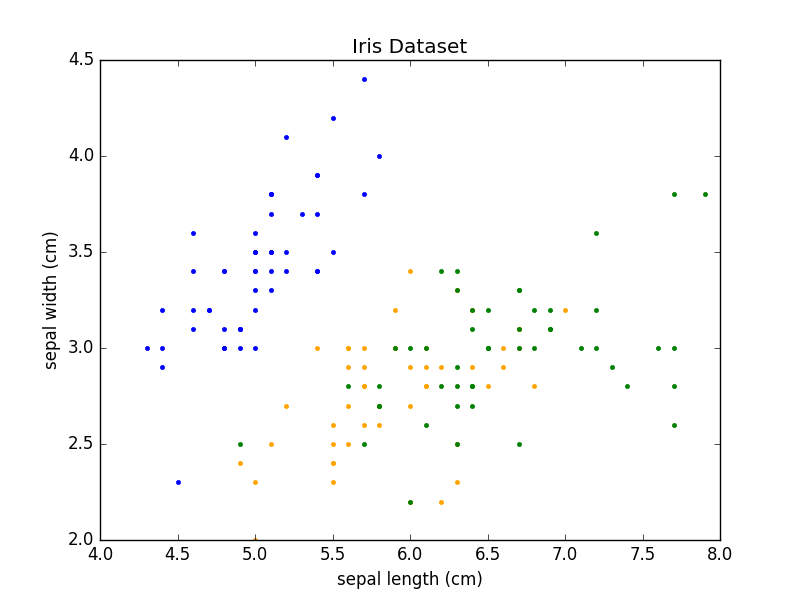
\includegraphics[scale=0.32]{imagenes/c6/IrisSet}
	\caption{Distribución de las dos primeras características de \textit{Iris Dataset}}\label{fig:figure27}
\end{figure}

\subsection{Conjuntos de datos artificiales}

En el caso de los conjuntos de datos artificiales el objetivo es generar clusters con una geometría concreta, para ello sólo son necesarios dos atributos ($x$ e $y$) y un número de muestras arbitrario.

La Figura \ref{fig:figure22} muestra los 4 conjuntos de datos generados de manera artificial. Por simplicidad nos referiremos a cada uno de ellos por su identificador en ingles, que aparece en la anotación bajo cada imagen.

\begin{figure}[bth]
	\myfloatalign
	\subfloat[\textit{Rand Dataset}]
	{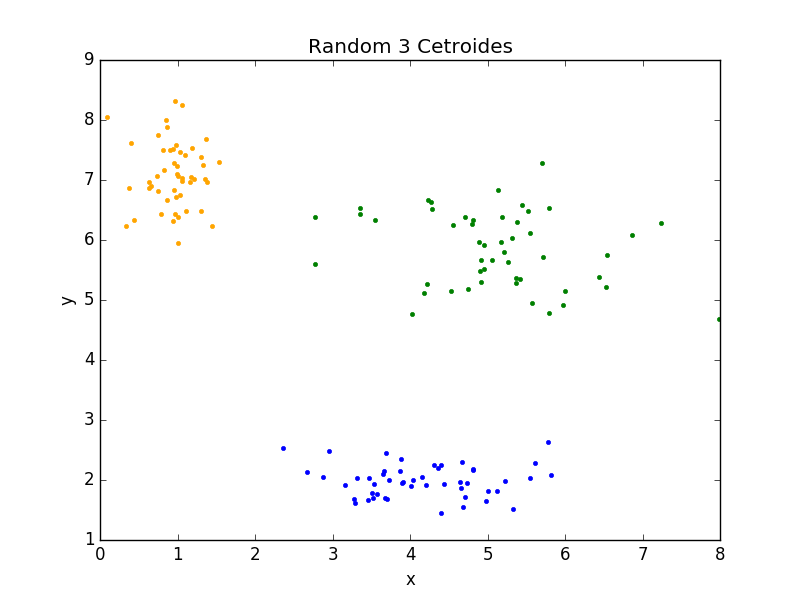
\includegraphics[width=.4\linewidth]{imagenes/c6/ArtifSets/RandSet}}
	\subfloat[\textit{Spirals Dataset}]
	{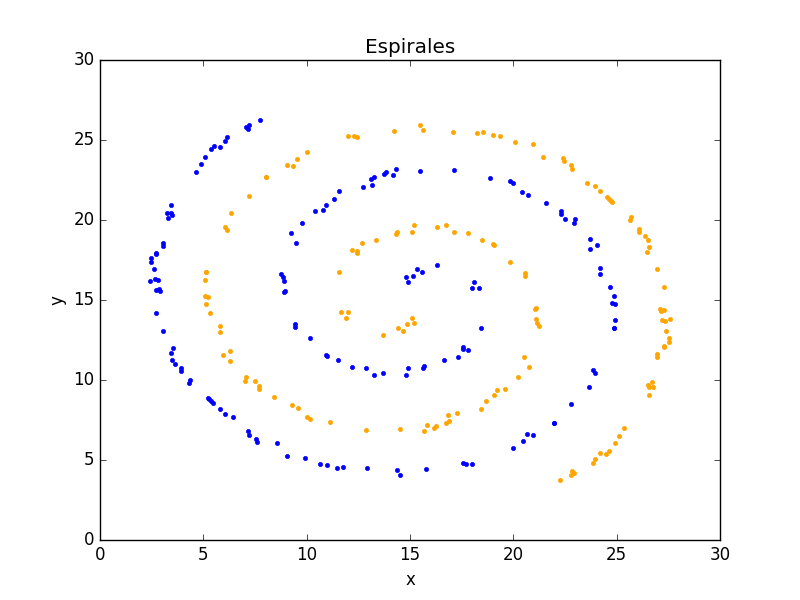
\includegraphics[width=.4\linewidth]{imagenes/c6/ArtifSets/SpiralSet}}\\
	\subfloat[\textit{Circles Dataset}]
	{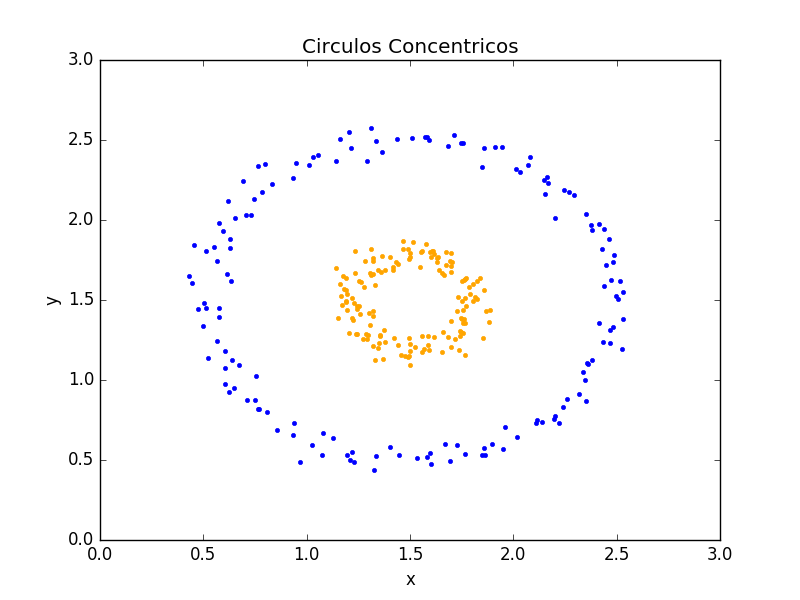
\includegraphics[width=.4\linewidth]{imagenes/c6/ArtifSets/Circles}}
	\subfloat[\textit{Moons Dataset}]
	{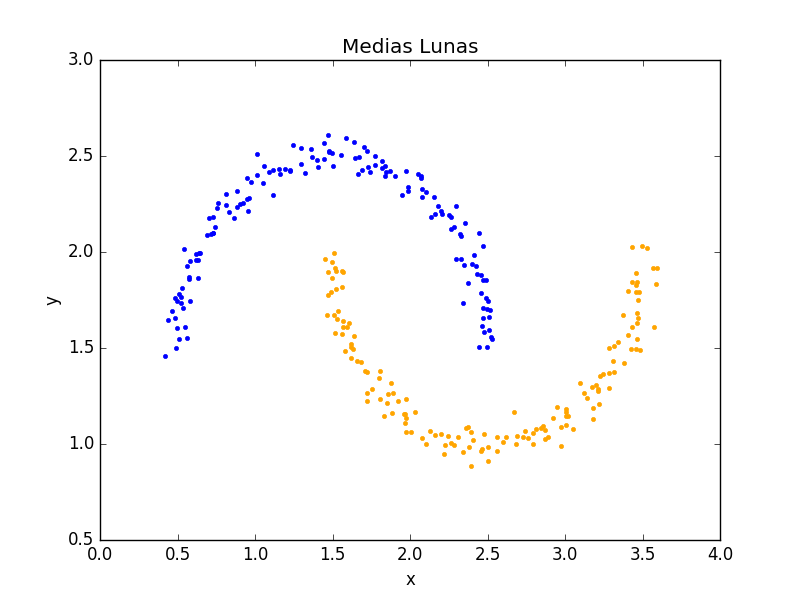
\includegraphics[width=.4\linewidth]{imagenes/c6/ArtifSets/MoonsSet}}
	\caption{Conjuntos de datos artificiales.}\label{fig:figure22}
\end{figure}

\section{Medida del error}

Tomamos la medida del error que Wagstaff et al. (2001) \cite{Wagstaff:2001b}, los autores de COP-K-medias, proponen en su trabajo para evaluar los resultados.

Dado que en la experimentación disponemos de las etiquetas verdaderas asociadas a cada uno de los conjuntos de datos, podemos hacer uso de las mismas en el post-procesado para evaluar los resultados que proporciona cada método.

Para calcular la exactitud de las predicciones resultado de cada método emplearemos \textit{Rand Index} \cite{Rand:1971}, que calcula el grado de similitud entre dos particiones dadas $P_1$ y $P_2$ del mismo conjunto de datos $X$.

Interpretamos cada partición como una colección de $n (n-1) / 2$ decisiones de emparejamiento, donde $n$ es el número de instancias en $X$. Para cada par de instancias $x_i$ y $x_j$ en $X$, $P_i$ las asigna al mismo cluster o a clusters diferentes. Tomamos $a$ como el número de emparejamientos donde $x_i$ está en el mismo cluster que $x_j$ en $P_1$ y $P_2$, y tomamos $b$ como el suceso contrario. Entonces, el grado de similitud entre $P_1$ y $P_2$ se calcula como:

\begin{equation}
Rand(P_1, P_2) = \frac{a + b}{n (n-1) / 2}
\label{eqn70}
\end{equation}

Esta será la medida del error que emplearemos en todos los experimentos.

\section{Generación de las restricciones}

Para generar las restricciones haremos uso de la función propuesta para ello en la Sección \ref{genConst}. La cantidad de restricciones viene definida como un porcentaje aplicado sobre el cardinal de conjunto de datos. Dicho porcentaje se especificará en la sección correspondiente al análisis de cada algoritmo. No obstante, podemos obtener una representación gráfica de las restricciones haciendo uso de las funcionalidades de la biblioteca Matplotlib, la Figura \ref{fig:figure23} muestra las restricciones generadas sobre los conjuntos de datos \textit{Rand Dataset} e \textit{Rand Dataset}, especificando que el número de restricciones debe ser un $30\%$ del total de los datos disponibles en cada caso.

\begin{figure}[bth]
	\myfloatalign
	\subfloat[\textit{Iris Dataset}]
	{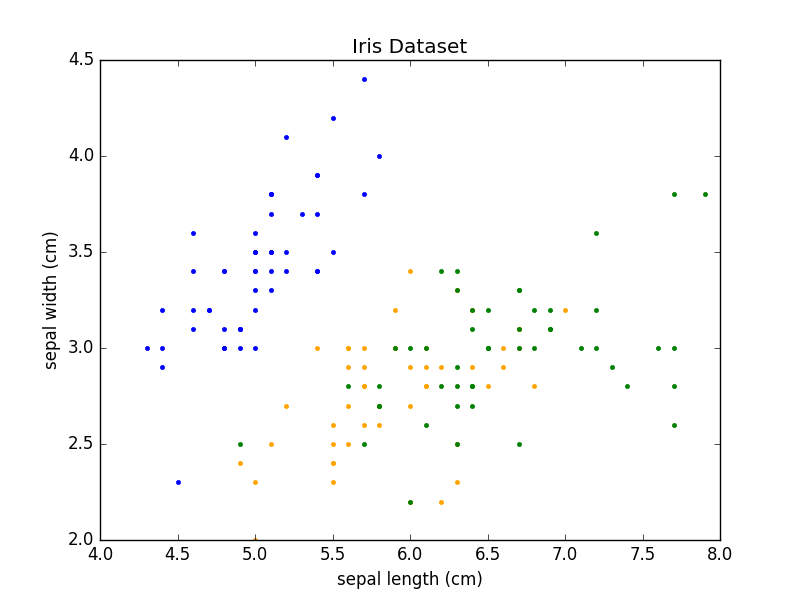
\includegraphics[width=.3\linewidth]{imagenes/c6/IrisSet}}
	\subfloat[Restricciones \acs{ML}]
	{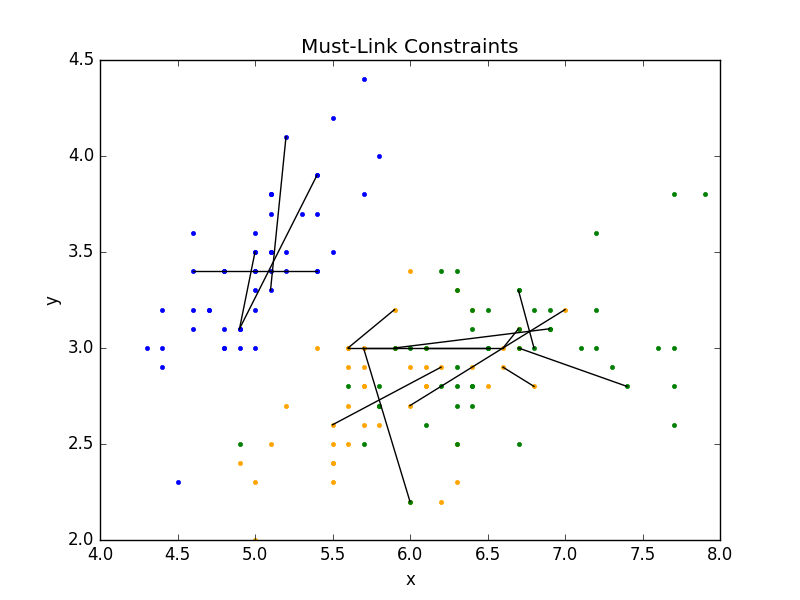
\includegraphics[width=.3\linewidth]{imagenes/c6/Restr/IrisML}}
	\subfloat[Restricciones \acs{CL}]
	{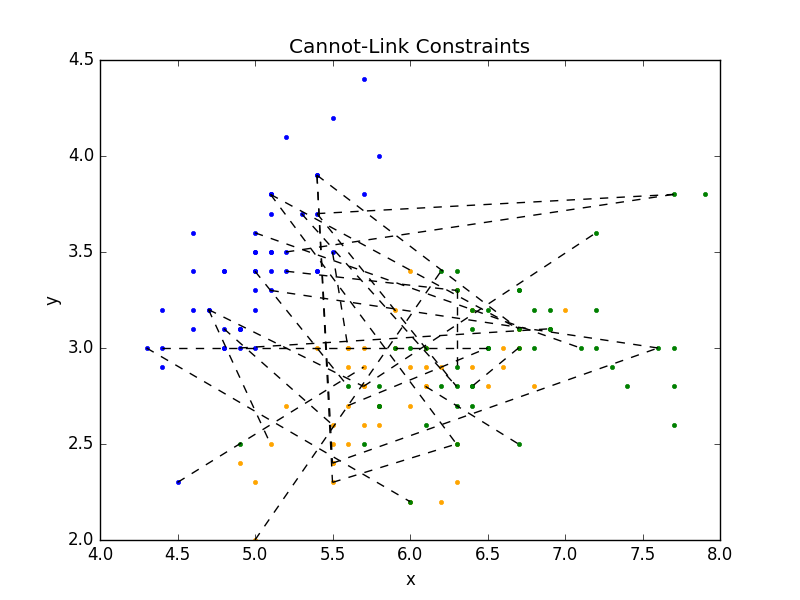
\includegraphics[width=.3\linewidth]{imagenes/c6/Restr/IrisCL}}\\
	\subfloat[\textit{Rand Dataset}]
	{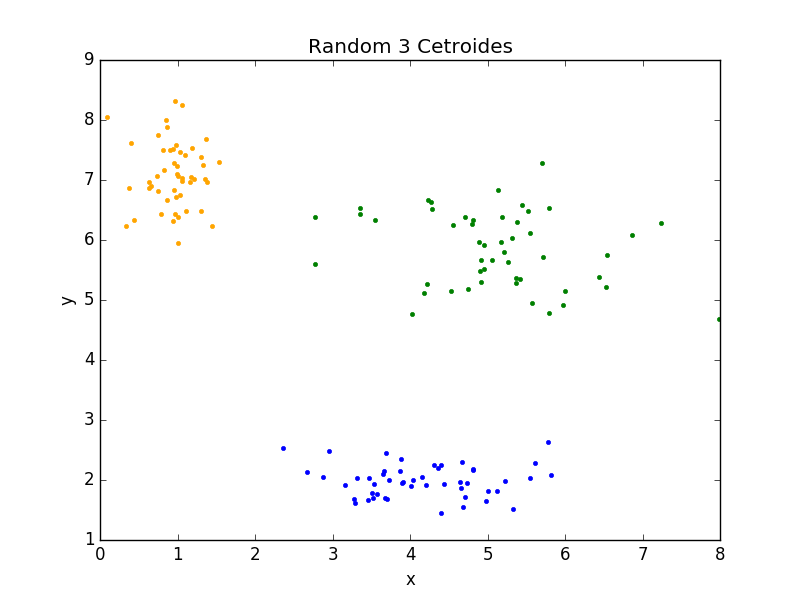
\includegraphics[width=.3\linewidth]{imagenes/c6/ArtifSets/RandSet}}
	\subfloat[Restricciones \acs{ML}]
	{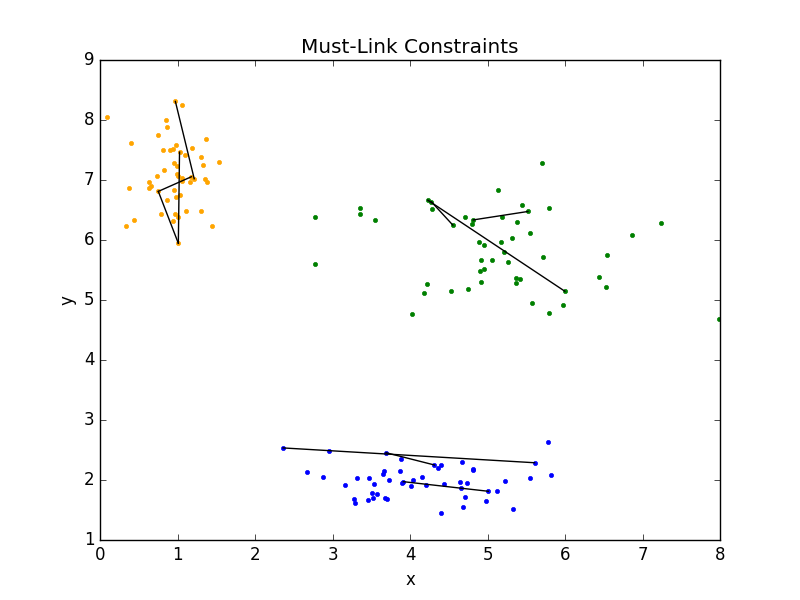
\includegraphics[width=.3\linewidth]{imagenes/c6/Restr/RandML}}
	\subfloat[Restricciones \acs{CL}]
	{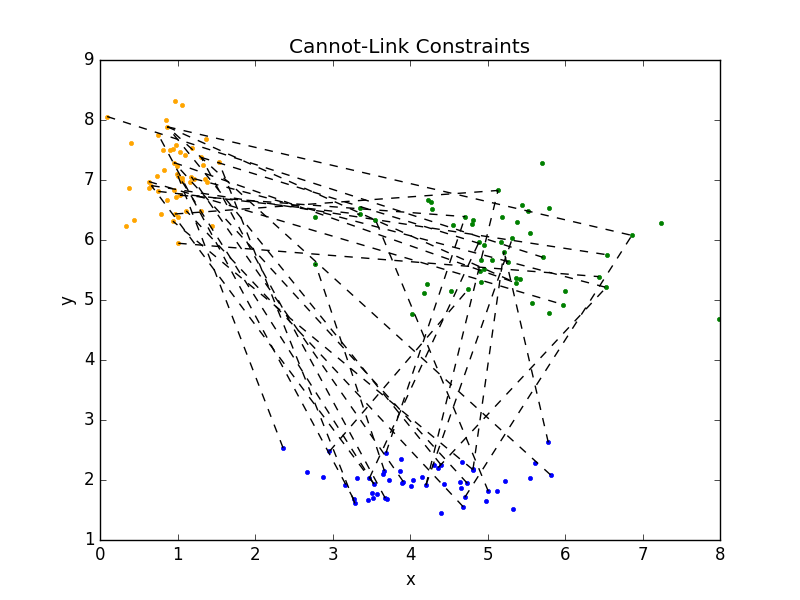
\includegraphics[width=.3\linewidth]{imagenes/c6/Restr/RandCL}}\\
	\caption{Visualización de las restricciones.}\label{fig:figure23}
\end{figure} 

\section{Resultados obtenidos con COP-K-Medias}

La Tabla \ref{tab:tabla5} muestra los resultados obtenidos al aplicar el algoritmo COP-K-Medias (Sección \ref{copkm}) a los conjuntos de datos presentados en la Sección \ref{datasets}. En ella se indican: el valor para \textit{Rand Index}, el tiempo que tarda el algoritmo en proporcionar salida, y el porcentaje de restricciones \acs{ML} y \acs{CL}. El número de restricciones generado para cada conjunto de datos es un $10\%$ del total de datos disponibles en cada caso, por tanto la suma del porcentaje de restricciones de los dos tipos debe ser aproximadamente $0.1$.

\begin{table}[!h]
	\centering
	\setlength{\arrayrulewidth}{1mm}
	\setlength{\tabcolsep}{10pt}
	\renewcommand{\arraystretch}{0.75}
	
	\rowcolors{2}{gray!25}{white}
	\begin{tabular}{ >{\centering\arraybackslash}m{2.5cm}  >{\centering\arraybackslash}m{1.8cm}>{\centering\arraybackslash}m{1.5cm}>{\centering\arraybackslash}m{1.2cm}>{\centering\arraybackslash}m{1.2cm}}
		\hline
		\rowcolor{black}
		\multicolumn{5}{c}{\bf \color{white}{Resultados de COP-K-Medias con restricciones CL y ML}}\\
		\hline
		\rowcolor{gray!50}
		\textbf{Dataset} & \textbf{RandIndex} & \textbf{Tiempo} & \textbf{\% ML} & \textbf{\% CL}  \\
		Iris & $0.499$ & $0.0532$ & $0.033$ & $0.066$ \\
		Wine & $0.38$ & $0.087$ & $0.056$ & $0.039$ \\
		Glass  & $0.25$ & $0.1449$ & $0.15$ & $0.04$ \\
		Breast Cancer & NA & NA & $0.028$ & $0.07$ \\ 
		Digits & $0.632$ & $13.306$ & $0.008$ & $0.092$ \\
		Rand & $0.960$ & $0.0346$ & $0.033$ & $0.066$ \\
		Spirals & $0.0245$ & $0.13$ & $0.05$ & $0.05$ \\
		Circles & $-0.002$ & $0.16$ & $0.046$ & $0.053$ \\
		Moons & NA & NA & $0.053$ & $0.046$ \\
		\hline
		
	\end{tabular}
	\caption{Resultados obtenidos con COP-K-Medias empleando restricciones \acs{CL} y \acs{ML}}
	\label{tab:tabla5}
\end{table}

De entre los resultados obtenidos destacan los asociados a los conjuntos de datos \textit{Glass Dataset} y \textit{Moons Dataset}. Encontramos que en ninguno de los dos casos el algoritmo COP-K-Medias es capaz de encontrar una solución factible, a pesar de que es seguro que esta existe, ya que las restricciones se generan en base a las etiquetas verdaderas. Esto es consecuencia directa de lo expuesto en la Observación \ref{ob:observacion34}, puesto que en la resolución del problema se emplean tanto restricciones de tipo \acs{ML} como \acs{CL}. Para obtener resultados para \textit{Glass Dataset} y \textit{Moons Dataset} podemos aplicar transformaciones a las restricciones para hacer el problema más simple (tratable), esto es, suprimir las restricciones de tipo \acs{CL} y aumentar las de tipo \acs{ML}, tal y como especificamos en la Sección \ref{Problemas}. La Tabla \ref{tab:tabla6} muestra los resultados con esta nueva configuración.

\begin{table}[!h]
	\centering
	\setlength{\arrayrulewidth}{1mm}
	\setlength{\tabcolsep}{10pt}
	\renewcommand{\arraystretch}{0.75}
	
	\rowcolors{2}{gray!25}{white}
	\begin{tabular}{ >{\centering\arraybackslash}m{2.5cm}  >{\centering\arraybackslash}m{1.8cm}>{\centering\arraybackslash}m{1.5cm}>{\centering\arraybackslash}m{1.2cm}>{\centering\arraybackslash}m{1.2cm}}
		\hline
		\rowcolor{black}
		\multicolumn{5}{c}{\bf \color{white}{Resultados de COP-K-Medias con restricciones ML}}\\
		\hline
		\rowcolor{gray!50}
		\textbf{Dataset} & \textbf{RandIndex} & \textbf{Tiempo} & \textbf{\% ML} & \textbf{\% CL}  \\
		Iris & $0.489$ & $0.0423$ & $0.366$ & $0$ \\
		Wine & $0.337$ & $0.0762$ & $0.353$ & $0$ \\
		Glass & $0.175$ & $0.112$ & $0.555$ & $0$ \\
		Breast Cancer & $0.45$ & $0.556$ & $0.224$ & $0$ \\
		Digits & $0.582$ & $10.847$ & $0.105$ & $0$ \\
		Rand & $1.0$ & $0.031$ & $0.393$ & $0$ \\
		Spirals & $-0.0028$ & $0.1302$ & $0.52$ & $0$ \\
		Circles & $0.091$ & $0.1301$ & $0.463$ & $0$ \\
		Moons & $0.126$ & $0.116$ & $0.513$ & $0$ \\
		\hline
		
	\end{tabular}
	\caption{Resultados obtenidos con COP-K-Medias empleando solo restricciones \acs{ML}}
	\label{tab:tabla6}
\end{table}

Como cabía esperar, los resultados de la Tabla \ref{tab:tabla6} muestran que empleado solo restricciones de tipo \acs{ML} el algoritmo COP-K-Medias es capaz de dar una partición para todos los conjuntos de datos. Sin embargo la precisión de las predicciones decrece en algunos casos, esto se debe la pérdida de la información que proporcionaban las restricciones \acs{CL}. 

Además de obtener los resultados numéricos podemos representar algunas de las particiones obtenidas con COP-K-Medias para obtener una mejor idea del comportamiento del algoritmo. En la Figura \ref{fig:figure24} se muestran los resultados obtenidos para \textit{Iris Dataset} y \textit{Rand Dataset}, los cuadros (a) y (b) muestran los resultados considerando restricciones ML y CL, mientras que los (c) y (d) solo consideran restricciones ML.

\begin{figure}[bth]
	\myfloatalign
	\subfloat[]
	{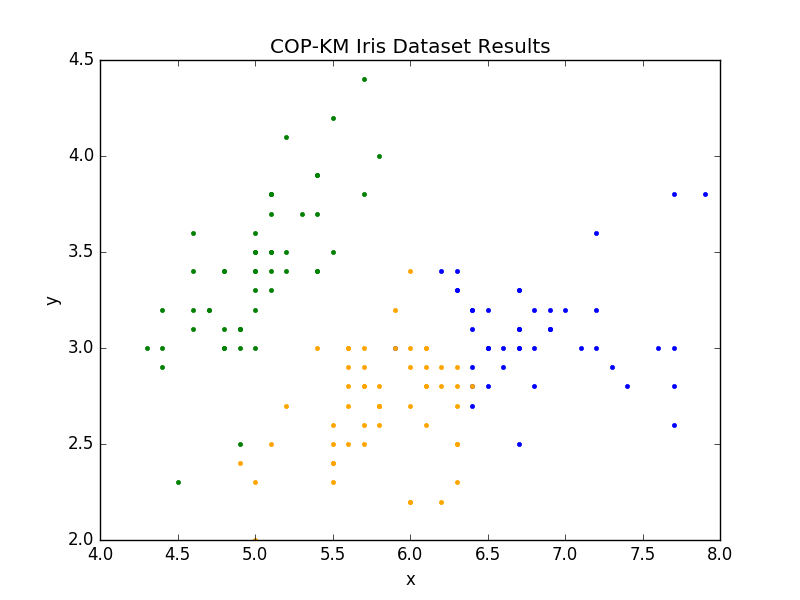
\includegraphics[width=.5\linewidth]{imagenes/c6/COPKM/Iris01}}
	\subfloat[]
	{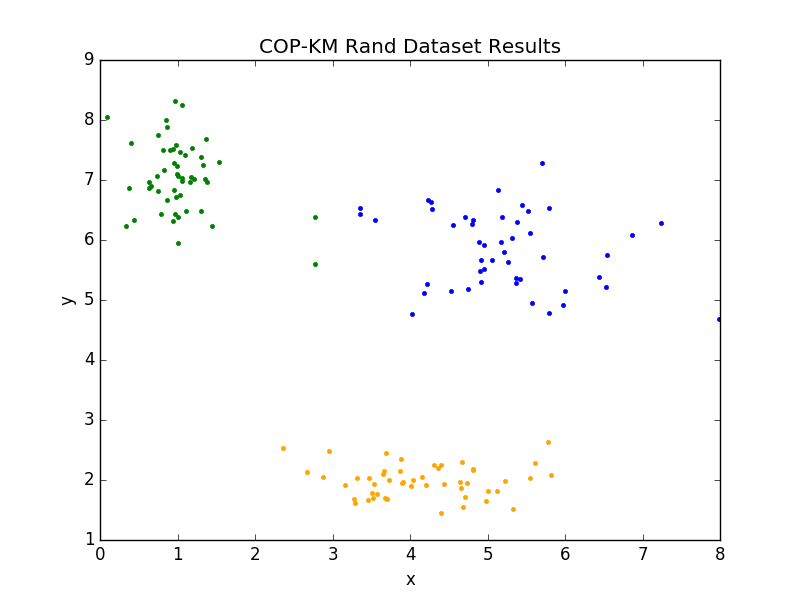
\includegraphics[width=.5\linewidth]{imagenes/c6/COPKM/Rand01}}\\
	\subfloat[]
	{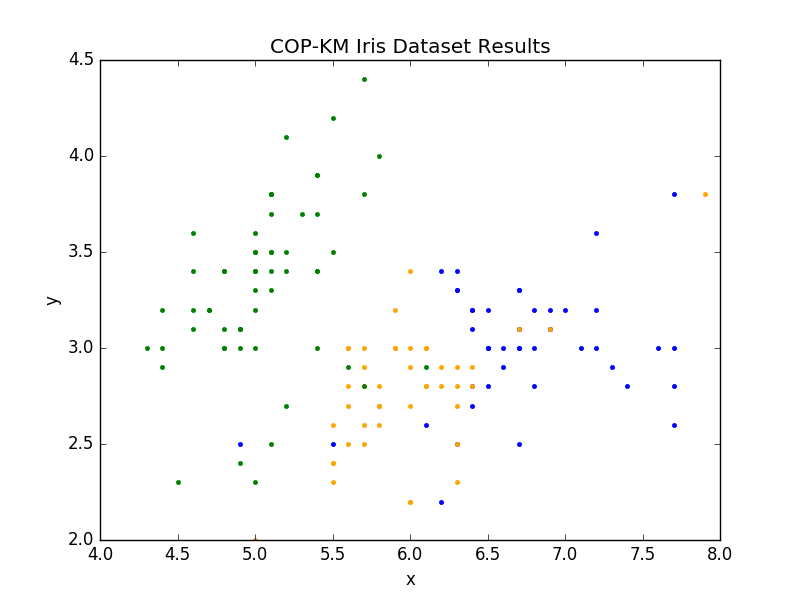
\includegraphics[width=.5\linewidth]{imagenes/c6/COPKM/IrisSoloML}}
	\subfloat[]
	{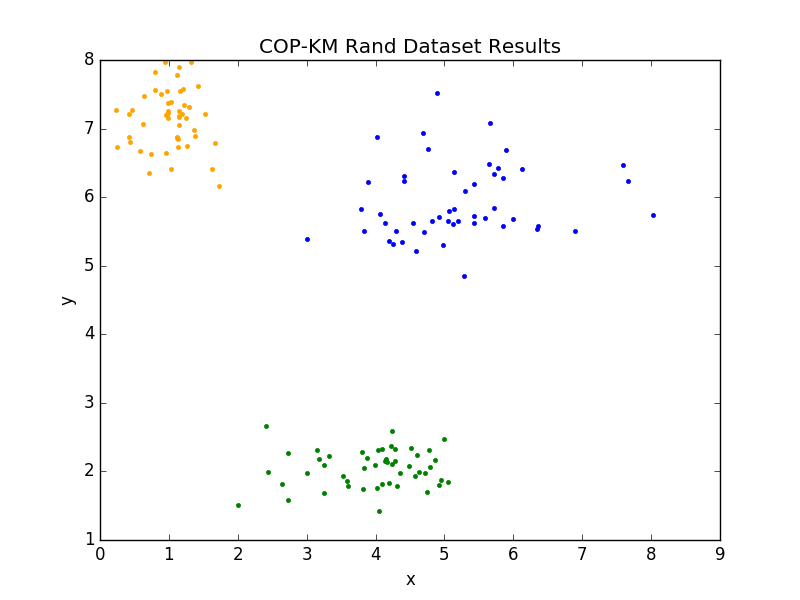
\includegraphics[width=.5\linewidth]{imagenes/c6/COPKM/RandSoloMl}}\\
	\caption{Visualización de los resultados de COP-K-Medias}\label{fig:figure24}
\end{figure}

En la Figura \ref{fig:figure24} destacan las instancias del conjunto de datos \textit{Iris Dataset} que parecen estar dentro de un cluster distinto al que pertenecen. Es en estos casos en los que destaca la influencia de las restricciones en el proceso de asignación de instancias a clusters, el algoritmo K-Medias (Apéndice \ref{ap:kmeans}) nunca proporcionaría esta partición como resultado.

\clearpage

\section{Resultados obtenidos con CEKM}

La Tabla \ref{tab:tabla8} muestra los resultados obtenidos al aplicar el algoritmo \acf{CEKM} (Sección \ref{cekm}) a los conjuntos de datos presentados en la Sección \ref{datasets}. Emplearemos un número de restricciones igual al $25\%$ del total de ejemplos disponibles para cada conjunto de datos. \footnote{Para obtener resultados con \acs{CEKM} para \textit{Breast Cancer Dataset} es necesario modificar el parámetro \texttt{stop\_thr}, y establecerlo a $0.1$ }

\begin{table}[!h]
	\centering
	\setlength{\arrayrulewidth}{1mm}
	\setlength{\tabcolsep}{10pt}
	\renewcommand{\arraystretch}{0.9}
	
	\rowcolors{2}{gray!25}{white}
	\begin{tabular}{ >{\centering\arraybackslash}m{2.5cm}  >{\centering\arraybackslash}m{1.8cm}>{\centering\arraybackslash}m{1.5cm}}
		\hline
		\rowcolor{black}
		\multicolumn{3}{c}{\bf \color{white}{Resultados obtenidos con CEKM}}\\
		\hline
		\rowcolor{gray!50}
		\textbf{Dataset} & \textbf{RandIndex} & \textbf{Tiempo}  \\
		Iris & $0.554$ & $9.567$  \\
		Wine & $0.395$ & $14.48$  \\
		Glass & NA & NA  \\
		Breast Cancer & $0.491$ & $64.22$  \\
		Digits & NA & NA  \\
		Rand & $0.950$ & $9.411$  \\
		Spirals & $0.061$ & $9.839$  \\
		Circles & $-0.0030$ & $12.588$  \\
		Moons & $0.247$ & $11.191$  \\
		\hline
		
	\end{tabular}
	\caption{Resultados obtenidos con \acs{CEKM}}
	\label{tab:tabla8}
\end{table}

En ella destacan los resultados obtenidos para los conjuntos de datos \textit{Glass Dataset} y \textit{Digits Dataset}. El algoritmo \acs{CEKM} no es capaz de dar resultado para estos dos conjuntos de datos, debido a que las estructuras de memoria que lo soportan crecen de manera exponencial con $K$. La figura \ref{fig:figure25} muestra los resultados obtenidos con \acs{CEKM} para los conjuntos de datos \textit{Iris Dataset} y \textit{Rand Dataset}.

\begin{figure}[bth]
	\myfloatalign
	\subfloat[Resultados para \textit{Iris Dataset}]
	{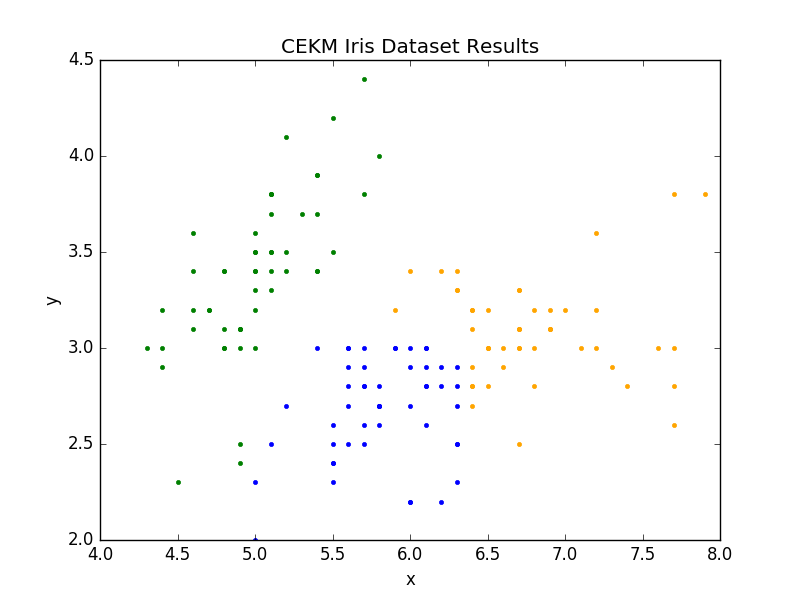
\includegraphics[width=.5\linewidth]{imagenes/c6/CEKM/CEKMIrisResult}}
	\subfloat[Resultados para \textit{Rand Dataset}]
	{\includegraphics[width=.5\linewidth]{imagenes/c6/CEKM/CEKMRandResult}}
	\caption{Visualización de los resultados de \acs{CEKM}}\label{fig:figure25}
\end{figure}

\clearpage

\section{Resultados obtenidos con LCVQE}

La Tabla \ref{tab:tabla8} muestra los resultados obtenidos al aplicar el algoritmo \acf{LCVQE} (Sección \ref{lcvqe}) a los conjuntos de datos presentados en la Sección \ref{datasets}. Daremos como parámetro para los centroides iniciales los calculados con el algoritmo K-Medias (Apéndice \ref{ap:kmeans}). Respecto al número de restricciones empleadas, será un $25\%$ del total de ejemplos disponibles para cada conjunto de datos.

\begin{table}[!h]
	\centering
	\setlength{\arrayrulewidth}{1mm}
	\setlength{\tabcolsep}{10pt}
	\renewcommand{\arraystretch}{0.9}
	
	\rowcolors{2}{gray!25}{white}
	\begin{tabular}{ >{\centering\arraybackslash}m{2.5cm}  >{\centering\arraybackslash}m{1.8cm}>{\centering\arraybackslash}m{1.5cm}}
		\hline
		\rowcolor{black}
		\multicolumn{3}{c}{\bf \color{white}{Resultados obtenidos con LCVQE}}\\
		\hline
		\rowcolor{gray!50}
		\textbf{Dataset} & \textbf{RandIndex} & \textbf{Tiempo}  \\
		Iris & $0.663$ & $0.141$  \\
		Wine & $0.390$ & $0.002$  \\
		Glass & $0.197$ & $0.002$  \\
		Breast Cancer & $0.616$ & $0.003$  \\
		Digits & $0.680$ & $0.062$  \\
		Rand & $0.989$ & $0.001$  \\
		Spirals & $0.057$ & $0.002$  \\
		Circles & $-0.003$ & $0.005$  \\
		Moons & $0.215$ & $0.002$  \\
		\hline
		
	\end{tabular}
	\caption{Resultados obtenidos con \acs{LCVQE}}
	\label{tab:tabla9}
\end{table}

De nuevo, podemos obtener una representación de algunos de los mejores resultados obtenidos con \acs{LCVQE}. La figura \ref{fig:figure26} muestra los resultados obtenidos con \acs{LCVQE} para los conjuntos de datos \textit{Iris Dataset} y \textit{Rand Dataset}. 


\begin{figure}[bth]
	\myfloatalign
	\subfloat[Resultados para \textit{Iris Dataset}]
	{\includegraphics[width=.5\linewidth]{imagenes/c6/LCVQE/LCVQEIris}}
	\subfloat[Resultados para \textit{Rand Dataset}]
	{\includegraphics[width=.5\linewidth]{imagenes/c6/LCVQE/LCVQERand}}
	\caption{Visualización de los resultados de \acs{LCVQE}}\label{fig:figure26}
\end{figure}

\clearpage

\section{Resultados obtenidos con RDP-Means}

La Tabla \ref{tab:tabla10} muestra los resultados obtenidos al aplicar el algoritmo \acf{RDPM} (Sección \ref{rdpmYtvc}) a los conjuntos de datos presentados en la Sección \ref{datasets}. Para aplicar \acs{RDPM} es necesario especificar el parámetro $\lambda$, en este caso este parámetro se calcula de manera experimental y en base a las distancia medias entre instancias dentro del conjunto de datos. De igual forma que en el caso anterior, especificaremos el número de restricciones como un $25\%$ del total de ejemplos disponibles para cada conjunto de datos.

\begin{table}[!h]
	\centering
	\setlength{\arrayrulewidth}{1mm}
	\setlength{\tabcolsep}{10pt}
	\renewcommand{\arraystretch}{0.85}
	
	\rowcolors{2}{gray!25}{white}
	\begin{tabular}{ >{\centering\arraybackslash}m{2.5cm}  >{\centering\arraybackslash}m{1.8cm}>{\centering\arraybackslash}m{1.5cm}>{\centering\arraybackslash}m{1cm}>{\centering\arraybackslash}m{1cm}}
		\hline
		\rowcolor{black}
		\multicolumn{5}{c}{\bf \color{white}{Resultados obtenidos con RDPM}}\\
		\hline
		\rowcolor{gray!50}
		\textbf{Dataset} & \textbf{RandIndex} & \textbf{Tiempo} & \textbf{$\lambda$} & \textbf{$K_{out}$}  \\
		Iris & $0.479$ & $0.508$ & $1.7$ & $3$ \\
		Wine & $0.342$ & $0.598$ & $438.11$ & $3$ \\
		Glass & $0.255$ & $0.785$ & $2.214$ & $6$ \\
		Breast Cancer & $0.501$ & $14.096$ & $2833.35$ & $3$ \\
		Digits & $0.665$ & $177.12$ & $44.14$ & $17$ \\
		Rand & $0.98$ & $0.365$ & $4$ & $3$ \\
		Spirals & $0.0147$ & $2.683$ & $13.83$ & $3$ \\
		Circles & $-0.003$ & $1.27$ & $1.5$ & $2$  \\
		Moons & $0.234$ & $1.563$ & $2$ & $2$ \\
		\hline
		
	\end{tabular}
	\caption{Resultados obtenidos con \acs{RDPM}}
	\label{tab:tabla10}
\end{table}

En la Tabla \ref{tab:tabla10} la columna $K_{out}$ representa el número de clases de la partición de salida proporcionada por \acs{LCVQE}. Podemos estudiar la influencia del parámetro $\lambda$ sobre este resultado, para ello ejecutamos el algoritmo especificando en cada cas un $\lambda$ mayor. La Tabla \ref{tab:tabla11} muestra los resultados obtenidos con esta nueva configuración.

\begin{table}[!h]
	\centering
	\setlength{\arrayrulewidth}{1mm}
	\setlength{\tabcolsep}{10pt}
	\renewcommand{\arraystretch}{0.85}
	
	\rowcolors{2}{gray!25}{white}
	\begin{tabular}{ >{\centering\arraybackslash}m{2.5cm}  >{\centering\arraybackslash}m{1.8cm}>{\centering\arraybackslash}m{1.5cm}>{\centering\arraybackslash}m{1cm}>{\centering\arraybackslash}m{1cm}}
		\hline
		\rowcolor{black}
		\multicolumn{5}{c}{\bf \color{white}{Resultados obtenidos con RDPM para un mayor $\lambda$}}\\
		\hline
		\rowcolor{gray!50}
		\textbf{Dataset} & \textbf{RandIndex} & \textbf{Tiempo} & \textbf{$\lambda_{mayor}$} & \textbf{$K_{out}$}  \\
		Iris & $0.321$ & $0.683$ & $2$ & $2$ \\
		Wine & $0.313$ & $0.691$ & $538.11$ & $3$ \\
		Glass & $0$ & $0.505$ & $4.214$ & $3$ \\
		Breast Cancer & $0.491$ & $11.236$ & $3833.35$ & $2$ \\
		Digits & $0.268$ & $144.96$ & $60.14$ & $4$ \\
		Rand & $0$ & $0.26$ & $7$ & $1$ \\
		Spirals & $0$ & $0.969$ & $20.5$ & $1$ \\
		Circles & $0$ & $0.965$ & $4.5$ & $1$  \\
		Moons & $0$ & $0.97$ & $5$ & $1$ \\
		\hline
		
	\end{tabular}
	\caption{Resultados obtenidos con \acs{RDPM} especificando un mayor $\lambda$}
	\label{tab:tabla11}
\end{table}

A la vista de los resultados expuestos en la Tabla \ref{tab:tabla11} podemos decir que escoger $\lambda$ es equivalente a escoger $K$ en los algoritmos que toman como parámetro el número de clusters de la partición de salida. Por tanto es crucial realizar un estudio sobre este parámetro para resolver el problema concreto al que nos enfrentemos. En la Figura \ref{fig:figure28} representamos los resultados obtenidos con las diferentes elecciones de $\lambda$ para los conjuntos de datos \textit{Iris Dataset} y \textit{Rand Dataset}. 

\begin{figure}[bth]
	\myfloatalign
	\subfloat[ \textit{Iris Dataset} con $\lambda = 1.7$]
	{\includegraphics[width=.5\linewidth]{imagenes/c6/RDPM/RDPMIris1}}
	\subfloat[ \textit{Iris Dataset} con $\lambda = 2$]
	{\includegraphics[width=.5\linewidth]{imagenes/c6/RDPM/RDPMIris2}}\\
	\subfloat[ \textit{Rand Dataset} con $\lambda = 4$]
	{\includegraphics[width=.5\linewidth]{imagenes/c6/RDPM/RDPMRand1}}
	\subfloat[ \textit{Rand Dataset} con $\lambda = 7$]
	{\includegraphics[width=.5\linewidth]{imagenes/c6/RDPM/RDPMRand2}}\\
	\caption{Visualización de los resultados de RDPM con diferentes valores de $\lambda$}\label{fig:figure28}
\end{figure}

La Figura \ref{fig:figure28} refleja claramente la influencia del parámetro $\lambda$ en la partición que \acs{RDPM} proporciona como resultado del proceso de clustering que lleva a cabo. En el caso del conjunto de datos \textit{Iris Dataset}, bastan 3 décimas de diferencia en $\lambda$ para que el resultado degenere en una partición de dos clusters en lugar de 3.

\clearpage

\section{Resultados obtenidos con TVClust}

La Tabla \ref{tab:tabla11} muestra los resultados obtenidos al aplicar el algoritmo \acf{TVClust} (Sección \ref{rdpmYtvc}) a los conjuntos de datos presentados en la Sección \ref{datasets}. Especificamos el número de restricciones como un $25\%$ del total de ejemplos disponibles para cada conjunto de datos, tal y como hicimos en los casos anteriores.

\begin{table}[!h]
	\centering
	\setlength{\arrayrulewidth}{1mm}
	\setlength{\tabcolsep}{10pt}
	\renewcommand{\arraystretch}{0.9}
	
	\rowcolors{2}{gray!25}{white}
	\begin{tabular}{ >{\centering\arraybackslash}m{2.5cm}  >{\centering\arraybackslash}m{1.8cm}>{\centering\arraybackslash}m{1.5cm}}
		\hline
		\rowcolor{black}
		\multicolumn{3}{c}{\bf \color{white}{Resultados obtenidos con TVClust}}\\
		\hline
		\rowcolor{gray!50}
		\textbf{Dataset} & \textbf{RandIndex} & \textbf{Tiempo}  \\
		Iris & $0.532$ & $0.342$  \\
		Wine & $0.176$ & $0.5$  \\
		Glass & $0.26$ & $3.332$  \\
		Breast Cancer & $0$ & $1.3$  \\
		Digits & $0.680$ & $78.46$  \\
		Rand & $0.941$ & $0.83$  \\
		Spirals & $0.042$ & $0.3$  \\
		Circles & $0.075$ & $1.7$  \\
		Moons & $0.576$ & $5.59$  \\
		\hline
		
	\end{tabular}
	\caption{Resultados obtenidos con \acs{TVClust}}
	\label{tab:tabla12}
\end{table}

Destaca el resultado obtenido para el conjunto de datos \textit{Breast Cancer Dataser}, para el que \acs{TVClust} no es capaz de encontrar una partición mínimamente acertada. Esto puede deberse a la alta dimensionalidad del conjunto de datos. La Figura \ref{fig:figure28} muestra los resultados obtenidos con \acs{TVClust} para los conjuntos de datos \textit{Iris Dataset} y \textit{Rand Dataset}. 


\begin{figure}[bth]
	\myfloatalign
	\subfloat[Resultados para \textit{Iris Dataset}]
	{\includegraphics[width=.5\linewidth]{imagenes/c6/TVClust/TVIris}}
	\subfloat[Resultados para \textit{Rand Dataset}]
	{\includegraphics[width=.5\linewidth]{imagenes/c6/TVClust/TVRand}}
	\caption{Visualización de los resultados de \acs{TVClust}}\label{fig:figure29}
\end{figure}

\clearpage

\section{Comparativa general de resultados}

La Tabla \ref{tab:tabla13} muestra los resultados obtenidos por cada algoritmo para cada conjunto de datos, en lo que a precisión en las predicciones se refiere. Salvo algunas excepciones, todos los algoritmos se comportan de manera similar bajo las condiciones descritas al inicio del Capítulo \ref{ch:Experimentación}. Destaca la precisión en las predicciones sobre el conjunto de datos \textit{Rand Dataset}, así como la pobreza de las mismas sobre el conjunto \textit{Circles Dataset}.

\begin{table}[!h]
	\centering
	\setlength{\arrayrulewidth}{1mm}
	\setlength{\tabcolsep}{9pt}
	\renewcommand{\arraystretch}{0.8}
	
	\rowcolors{2}{gray!25}{white}
	\begin{tabular}{ >{\centering\arraybackslash}m{2.5cm}  >{\centering\arraybackslash}m{1.2cm}>{\centering\arraybackslash}m{1.1cm}>{\centering\arraybackslash}m{1.1cm}>{\centering\arraybackslash}m{1.1cm}>{\centering\arraybackslash}m{1.3cm}}
		\hline
		\rowcolor{black}
		\multicolumn{6}{c}{\bf \color{white}{Comparativa General de Resultados (RandIndex)}}\\
		\hline
		\rowcolor{gray!50}
		\textbf{Dataset} & \textbf{COPKM} & \textbf{CEKM} & \textbf{LCVQE} & \textbf{RDPM} & \textbf{TVClust}  \\
		Iris & $0.489$  & $0.554 $ & $0.663 $ & $0.479 $ & $0.532 $ \\
		Wine & $0.337$  & $0.395 $ & $0.390 $ & $0.342 $ & $0.176 $ \\
		Glass & $0.175$  & NA & $0.197 $ & $0.255 $ & $0.26 $ \\
		Breast Cancer & $0.45$ & $0.491 $ & $0.616 $ & $0.501 $ & $0 $ \\
		Digits & $0.582$ & NA & $0.680 $ & $0.665 $ & $0.680 $ \\
		Rand & $1.0$ & $0.950 $ & $0.989 $ & $0.98 $ & $0.941 $ \\
		Spirals & $-0.0028$ & $0.061 $ & $0.057 $ & $0.0147 $ & $0.042 $ \\
		Circles & $0.091$  & $-0.003 $ & $-0.003 $ & $-0.003 $ & $0.075 $ \\
		Moons & $0.126$  & $0.247 $ & $0.215$ & $0.234 $ & $0.576 $ \\
		\hline
		
	\end{tabular}
	\caption{Comparativa general de resultados (RandIndex)}
	\label{tab:tabla13}
\end{table}

En lo que a tiempo de ejecución se refiere, la Tabla \ref{tab:tabla14} muestra las marcas obtenidas por cada algoritmo. Cabe destacar que, en los casos en los que un método toma menos de 1 segundo en proporcionar resultado, cualquier otro proceso ejecutando en la máquina puede perturbar las mediciones, por tanto no han de tomarse como medidas exactas, simplemente como indicadores generales.

\begin{table}[!h]
	\centering
	\setlength{\arrayrulewidth}{1mm}
	\setlength{\tabcolsep}{9pt}
	\renewcommand{\arraystretch}{0.8}
	
	\rowcolors{2}{gray!25}{white}
	\begin{tabular}{ >{\centering\arraybackslash}m{2.5cm}  >{\centering\arraybackslash}m{1.2cm}>{\centering\arraybackslash}m{1.1cm}>{\centering\arraybackslash}m{1.1cm}>{\centering\arraybackslash}m{1.1cm}>{\centering\arraybackslash}m{1.3cm}}
		\hline
		\rowcolor{black}
		\multicolumn{6}{c}{\bf \color{white}{Comparativa General de Resultados (Tiempo)}}\\
		\hline
		\rowcolor{gray!50}
		\textbf{Dataset} & \textbf{COPKM} & \textbf{CEKM} & \textbf{LCVQE} & \textbf{RDPM} & \textbf{TVClust}  \\
		Iris & $0.0423 $  & $9.567 $ & $0.141 $ & $0.508 $ & $0.683 $ \\
		Wine & $0.0762 $  & $14.48 $ & $0.002 $ & $0.598 $ & $0.691 $ \\
		Glass & $0.112 $  & NA & $0.002 $ & $0.785 $ & $0.505 $ \\
		Breast Cancer & $0.556 $ & $64.22 $ & $0.003 $ & $14.096 $ & $11.236 $\\
		Digits & $10.847 $ & NA & $0.062 $ & $177.12 $ & $144.96 $ \\
		Rand & $0.031 $ & $9.411 $ & $0.001 $ & $0.365 $ & $0.26 $ \\
		Spirals & $0.1302 $ & $9.839 $ & $0.002 $ & $2.683 $ & $0.969 $ \\
		Circles & $0.1301 $ & $12.588 $ & $0.005  $ & $1.27 $ & $0.965 $ \\
		Moons & $0.116 $ & $11.191 $ & $0.002 $ & $1.563 $ & $0.97 $ \\
		\hline
		
	\end{tabular}
	\caption{Comparativa general de resultados (Tiempo)}
	\label{tab:tabla14}
\end{table}


%\include{Chapters/Chapter01}
\cleardoublepage
% ********************************************************************
% Backmatter
%*******************************************************
\appendix
%********************************************************************
% Appendix
\chapter{El algoritmo k-medias}\label{ap:kmeans}

El algoritmo \acf{KM} es el método básico para aplicar clustering, fue ideado por  Hugo Steinhaus en 1957, aunque no fue aplicado a un caso real hasta 1967, por James MacQueen \cite{KMEANS:1967}. 

El procedimiento que aplica K-medias es simple: asignar cada instancia al cluster cuyo centroide se encuentre mas cercano a ella, y calcular los centroides en base a las instancias asignadas al cluster asociado a cada uno. De esta manera, siguiendo la notación introducida en la sección \ref{ch:Algoritmos}, la regla de actualización de los centroides es:

\begin{equation}
v_i = \frac{1}{|c_i|} \sum_{x_i \in c_i} x_i
\label{a1}
\end{equation}

Así, si cada instancia se asigna al cluster correspondiente al centroide mas cercano, la función de error que minimiza K-medias es:

\begin{equation}
ERR = \frac{1}{2} \sum_{j = i}^{k} \sum_{x_i \in c_i} (v_j - x_i)^2
\label{a2}
\end{equation}

Formalizando la regla de asignación obtenemos:

\begin{equation}
c^i = argmin(||x_i - v_j||^2) \;\; t.q. \;\; j \in \{1, \cdots, k\}
\label{a3}
\end{equation}

donde $c^i$ representa el cluster seleccionado para la instancia $x_i$. Con todo, el proceso que K-medias sigue para obtener una partición de los datos queda resumido en el algoritmo \ref{alg:kmedias}.

\begin{algorithm}
	
	\BlankLine
	\KwIn{Conjunto de datos $X$, numero de cluster resultantes $k$.}
	\KwOut{Partición $P$ del conjunto de datos $X$, centroides $V$.}
	\BlankLine
	\textbf{función} K-medias($X$, $k$) \Begin{
		\BlankLine
		1. Inicalización aleatoria de los centroides $V = \{v_1, \cdots, v_k\}$.\\
		2. Asignar cada instancia $x_i \in X$, al centroide más cercano $c_j$ siguiendo la ecuación \ref{a3}.\\
		3. Para cada cluster $c_i$, actualizar su centroide aplicando la ecuación \ref{a1}\\
		4. Iterar entre (2.) y (3.) hasta converger.\\
		5. \KwRet $C$, $V$
		\BlankLine
	}
	\BlankLine
	\caption{K-medias}
	\label{alg:kmedias}
\end{algorithm}



% Other Stuff in the Back
%*******************************************************
\cleardoublepage%********************************************************************
% Bibliography
%*******************************************************
% work-around to have small caps also here in the headline
% https://tex.stackexchange.com/questions/188126/wrong-header-in-bibliography-classicthesis
% Thanks to Enrico Gregorio
\defbibheading{bibintoc}[\bibname]{%
  \phantomsection
  \manualmark
  \markboth{\spacedlowsmallcaps{#1}}{\spacedlowsmallcaps{#1}}%
  \addtocontents{toc}{\protect\vspace{\beforebibskip}}%
  \addcontentsline{toc}{chapter}{\tocEntry{#1}}%
  \chapter*{#1}%
}
\printbibliography[heading=bibintoc]

% Old version, will be removed later
% work-around to have small caps also here in the headline
%\manualmark
%\markboth{\spacedlowsmallcaps{\bibname}}{\spacedlowsmallcaps{\bibname}} % work-around to have small caps also
%\phantomsection
%\refstepcounter{dummy}
%\addtocontents{toc}{\protect\vspace{\beforebibskip}} % to have the bib a bit from the rest in the toc
%\addcontentsline{toc}{chapter}{\tocEntry{\bibname}}
%\label{app:bibliography}
%\printbibliography

\cleardoublepage%*******************************************************
% Declaration
%*******************************************************
\refstepcounter{dummy}
\pdfbookmark[0]{Declaration}{declaration}
\chapter*{Declaration}
\thispagestyle{empty}
Put your declaration here.
\bigskip

\noindent\textit{\myLocation, \myTime}

\smallskip

\begin{flushright}
    \begin{tabular}{m{5cm}}
        \\ \hline
        \centering\myName \\
    \end{tabular}
\end{flushright}

\cleardoublepage\pagestyle{empty}

\hfill

\vfill


\pdfbookmark[0]{Colophon}{colophon}
\section*{Colofón}

Este documento ha sido redactado siguiendo el estilo tipográfico \texttt{classicthesis}, desarrollado por Andr\'e Miede y Ivo Pletikosić. Dicho estilo esta inspirado en el libro sobre tipografía ``\emph{The Elements of Typographic Style}''. \texttt{classicthesis} esta disponible para \LaTeX\ y \mLyX en:

\begin{center}
	\url{https://bitbucket.org/amiede/classicthesis/}
\end{center}

\bigskip

%\noindent\finalVersionString

%Hermann Zapf's \emph{Palatino} and \emph{Euler} type faces (Type~1 PostScript fonts \emph{URW
%Palladio L} and \emph{FPL}) are used. The ``typewriter'' text is typeset in \emph{Bera Mono},
%originally developed by Bitstream, Inc. as ``Bitstream Vera''. (Type~1 PostScript fonts were made
%available by Malte Rosenau and
%Ulrich Dirr.)

%\paragraph{note:} The custom size of the textblock was calculated
%using the directions given by Mr. Bringhurst (pages 26--29 and
%175/176). 10~pt Palatino needs  133.21~pt for the string
%``abcdefghijklmnopqrstuvwxyz''. This yields a good line length between
%24--26~pc (288--312~pt). Using a ``\emph{double square textblock}''
%with a 1:2 ratio this results in a textblock of 312:624~pt (which
%includes the headline in this design). A good alternative would be the
%``\emph{golden section textblock}'' with a ratio of 1:1.62, here
%312:505.44~pt. For comparison, \texttt{DIV9} of the \texttt{typearea}
%package results in a line length of 389~pt (32.4~pc), which is by far
%too long. However, this information will only be of interest for
%hardcore pseudo-typographers like me.%
%
%To make your own calculations, use the following commands and look up
%the corresponding lengths in the book:
%\begin{verbatim}
%    \settowidth{\abcd}{abcdefghijklmnopqrstuvwxyz}
%    \the\abcd\ % prints the value of the length
%\end{verbatim}
%Please see the file \texttt{classicthesis.sty} for some precalculated
%values for Palatino and Minion.
%
%    \settowidth{\abcd}{abcdefghijklmnopqrstuvwxyz}
%    \the\abcd\ % prints the value of the length

% ********************************************************************
% Game Over: Restore, Restart, or Quit?
%*******************************************************
\end{document}
% ********************************************************************

%bibtex MemoriaTFG.aux 
